\begin{savequote}[8cm]
\textlatin{Neque porro quisquam est qui dolorem ipsum quia dolor sit amet, consectetur, adipisci velit...}

There is no one who loves pain itself, who seeks after it and wants to have it, simply because it is pain...
  \qauthor{--- Cicero's \textit{de Finibus Bonorum et Malorum}}
\end{savequote}

\chapter{\label{ch:techniques}New Techniques in Selection Development} 
\minitoc

The upgraded detector has enhanced measuring capabilities, which is especially important for hadrons,
As hadrons tend to have much shorter tracks and are conventionally harder to reconstruct in scintillator detectors compared to muons, the explored hadronic kinematic phase space has been relatively restricted, and the reconstructed hadronic variables have relatively large uncertainties.
Since more exclusive event topologies, such as $\numuccopiop$, allow the measurement of high-level variables like the Transverse Kinematic Imbalance (TKI) variables, which provide invaluable insights on neutrino-nucleus interactions, it is highly desirable to reconstruct hadrons, measure their kinematic properties as precisely as possible, and explore their phase space as extensively as possible.

Two of the most common product hadrons from neutrino-nucleus interactions are protons and pions. 
The default particle identification and momentum reconstruction have been developed by colleagues at T2K using the Boosted Decision Tree (BDT) algorithm. The BDT algorithm has good performance, but it is still lacking in some aspects.
For instance, as it uses only single-track information, it cannot effectively distinguish between pions and muons. 
It can reconstruct proton momentum with an excellent resolution of about $3.5\%$, but it is insufficient for TKI analysis, which is highly sensitive to hadron kinematics. 

To address these gaps, I have developed and implemented new techniques for both hadrons, exploiting the precise position and $\dedx$ measurements and timing resolution.
For pions, I have invented the pion trackless reconstruction, a novel technique to reconstruct pions without requiring the presence of a reconstructed track, thereby lowering the detection threshold and significantly increasing reconstruction efficiency for low-momentum pions. 
As for protons, I have adapted the Elastically Scattered and Contained (ESC) protons technique~\cite{Lu:2016mjf}, first implemented in MINERvA, to demonstrate significant improvement in proton momentum reconstruction resolution, to SFGD. 
These new techniques are applied in the development of two signal sample selections, namely the $\numucczpiop$-ESC selection and the $\numuccopi$-TL selection, where the ``TL'' refers to the use of the trackless reconstruction technique.
Additionally, to prepare for the data-MC comparisons and future cross-section analysis, I have also developed a stopping pion control sample selection.

\section{$\numucczpiop$-ESC}
\label{sec:sel-esc}
     The $\numucczpiop$-ESC adds an additional ESC selection step to the $\numucczpiop$ selection developed by a T2K colleague.
     The details of the ESC step are elaborated below.
   %------------------- ESC ----------------%
    \subsection{Working Principles}
    \label{sec:sel-esc-wp}
     Protons stopping at rest deposit a large amount of energy—the so-called Bragg Peak—just before stopping.
     These protons tend to have their momenta better reconstructed as their momentum is more strongly correlated with their range. 
     As shown in Fig.~\ref{fig:dedx-pprres-eg}, protons having energy deposits below $1000$ units show large variances in momentum reconstruction. 

    \begin{figure}[h]
        \centering
        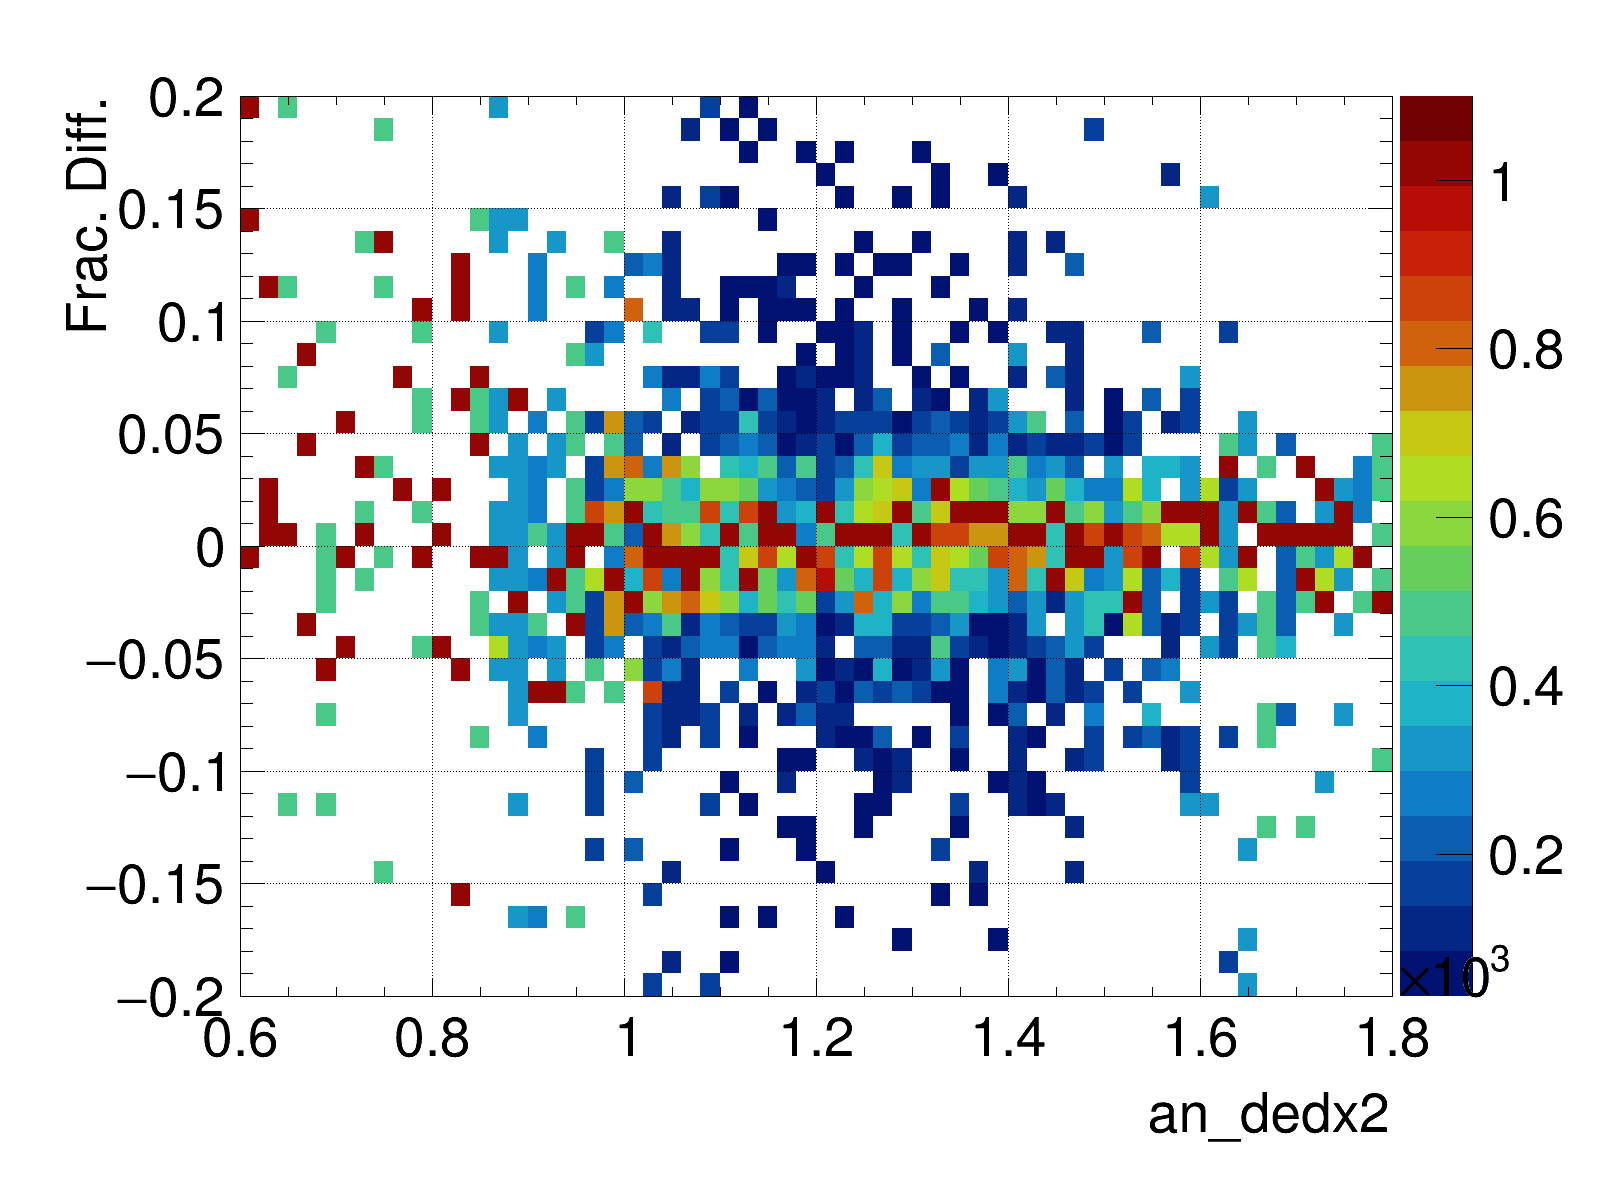
\includegraphics[width=\sgfidwid\linewidth]{figures/sel/an_dedx2_colnor_vs_p_pr_res_hist2d_al12_zoom.png}
        \caption{Proton momentum fractional difference against energy deposited at the third last node.}
        \label{fig:dedx-pprres-eg}
    \end{figure}
     Hence, these protons can be selected by placing a lower boundary cut on the energy deposited at the nodes near the end of the reconstructed tracks to obtain a sample with high proton momentum resolution.   
    
   \subsection{Implementation}
   \label{sec:sel-esc-imp}
	As the ESC selection is based on $\dedx$ at the end of the proton track, accurate reconstruction of $\dedx$ must first be obtained.
	To investigate the proper way of estimating $\dedx$, I have simulated multiple particle gun (PGUN) samples with protons traveling in different directions in the SFGD.
	More specifically, three samples travel along the $x$-, $y$-, and $z$-axes, and five other samples travel at $15^\circ$, $30^\circ$, $45^\circ$, $60^\circ$, and $75^\circ$ to the $x$-axis in the $x$-$z$ plane.
	As the proton direction should not affect its energy deposition, distinct characteristics of $\dedx$ along the proton trajectory can be utilized to validate the quality of the reconstructed $\dedx$.
	Besides the Bragg peak, another distinct feature of $\dedx$ is the minimal ionizing particle (MIP) region, where particles at high momentum traverse the scintillator depositing the minimal amount of energy. 
	Hence, the $\dedx$ remains at a relatively constant value for all such particles.
	When the $\dedx$ at the end of the proton tracks is plotted, besides the Bragg peak at large $\dedx$ corresponding to protons stopping at rest, there should be another peak at smaller $\dedx$ corresponding to protons that undergo secondary interactions and thus stop prematurely while still possessing high momentum.

	The first attempt is to use the smoothed energy directly. 
	Fig.~\ref{subfig:esc-smooth-e} plots energy deposits for the third to sixth nodes from the end for all PGUN samples traveling at non-orthogonal angles.
	It is reassuring to indeed observe the two peaks, the MIP peak and the Bragg peak, as hypothesized. 
  \begin{figure}
        \centering
        \begin{subfigure}[b]{\dbfigwid\textwidth}
             \centering
             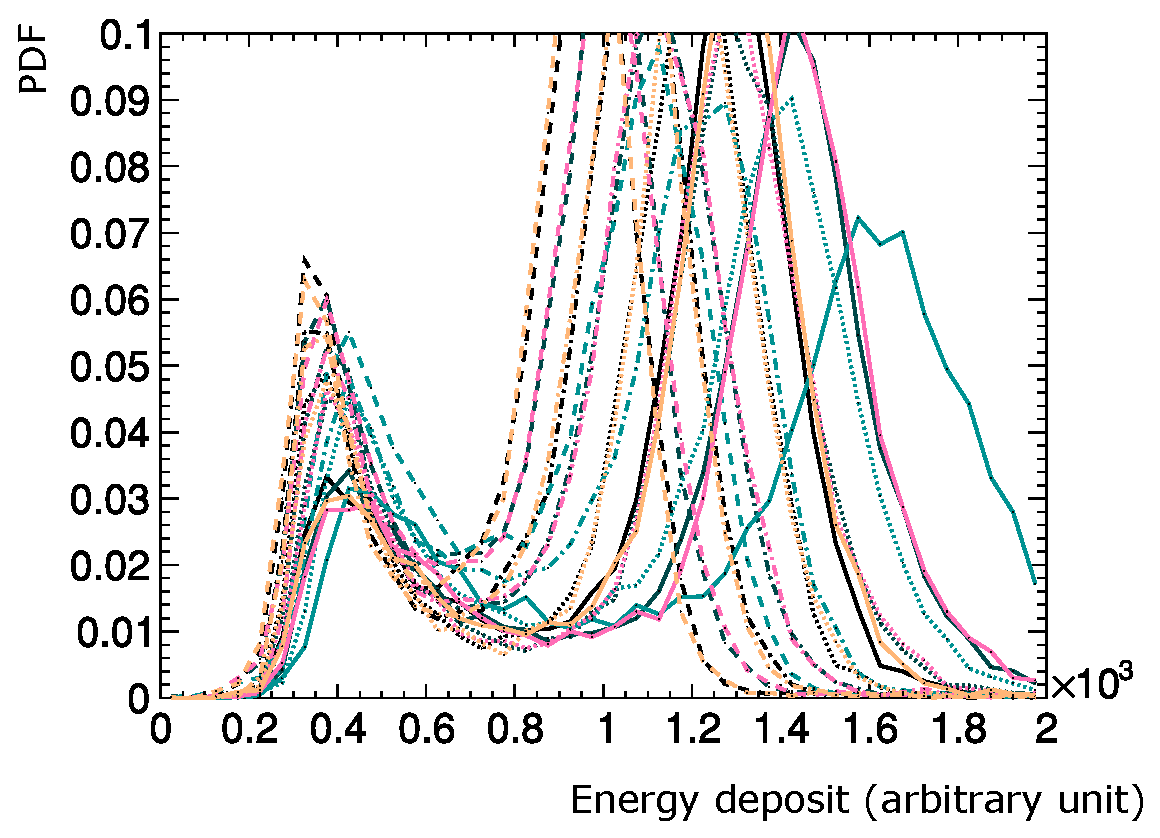
\includegraphics[width=\textwidth]{figures/sel/dedx5_pdf_skew_smooth_labelled.eps}
             \caption{Smoothed energy}
             \label{subfig:esc-smooth-e}
        \end{subfigure}
        \begin{subfigure}[b]{\dbfigwid\textwidth}
             \centering
             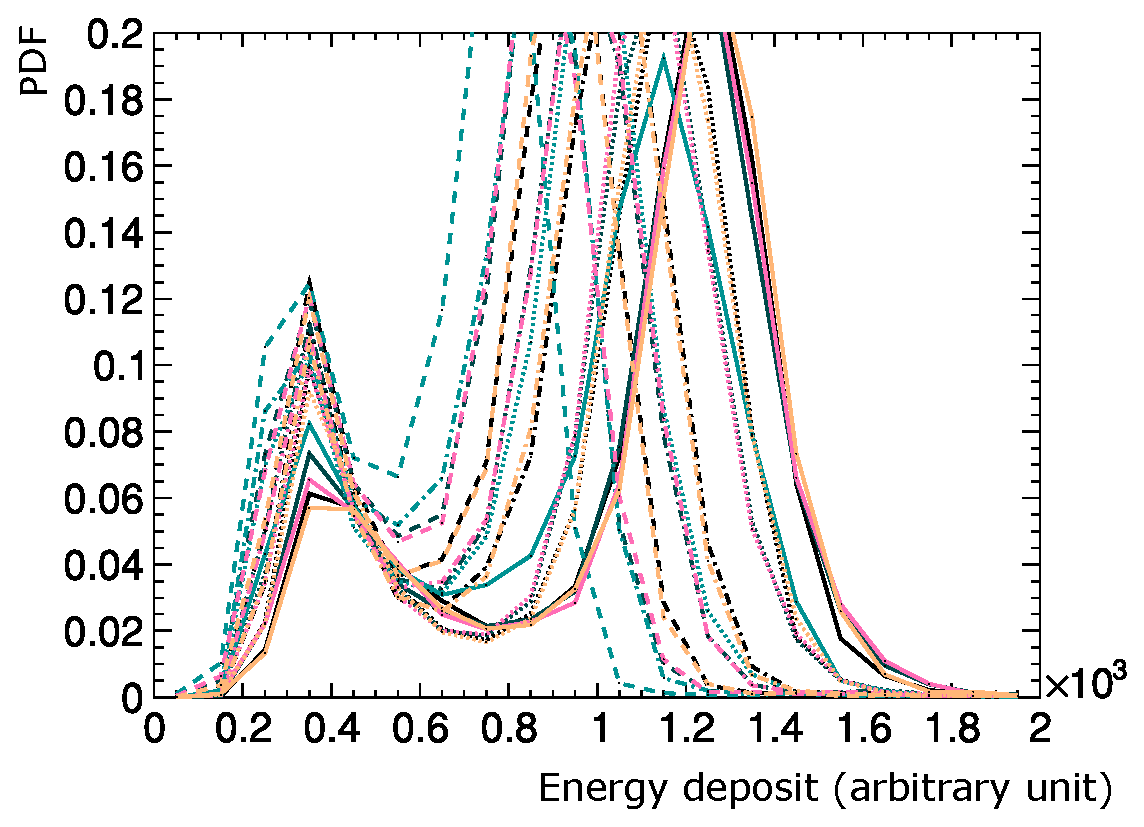
\includegraphics[width=\textwidth]{figures/sel/an_dedx5_pdf_skew_smooth_angnorm_labelled.eps}
             \caption{Angle-normalized smoothed energy}
             \label{subfig:esc-an-smooth-e}
        \end{subfigure}
        \caption{$\dedx$ estimation.}
        \label{fig:esc-angnorm}
  \end{figure}
     However, there are still some discrepancies.
     The MIP peaks are close to each other, but their positions differ noticeably.
     This is due to the different grouping of hits into nodes for protons traveling in different directions.
     The different numbers of hits in a node lead to different distances between nodes, so using the energy deposited per node as an estimation of $\dedx$ is not strictly valid.
     To account for the different propagation directions, I divided the energy by the sine of the angle between the trajectory and the $z$-axis.
     The angle-normalized energy is plotted in Fig.~\ref{subfig:esc-an-smooth-e}, which demonstrates that the angle-normalization step has achieved its goal—all MIP peaks have the same position.
     Hence, the angle-normalized energy can serve as a good reconstruction of $\dedx$ for the ESC selection.

     The multiple PGUN samples are combined into one large sample to determine suitable threshold $\dedx$ values.
     While plots like Fig.~\ref{fig:dedx-pprres-eg} clearly show the underlying idea of the ESC selection, profile plots are better suited for determining proper thresholds, as shown in Fig.~\ref{fig:esc-andedx-slice}.
     For example, Fig.~\ref{subfig:ans-dedx0-ppr-slice} shows large fluctuations below $200$, where a cut should be palced to exclude events below.
     Similarly, the threshold values for the other nodes are $500$, $1000$, $900$, $840$, and $740$ respectively.

  \begin{figure}[t]
      \centering
      \begin{subfigure}{\dbfigwid\textwidth}
           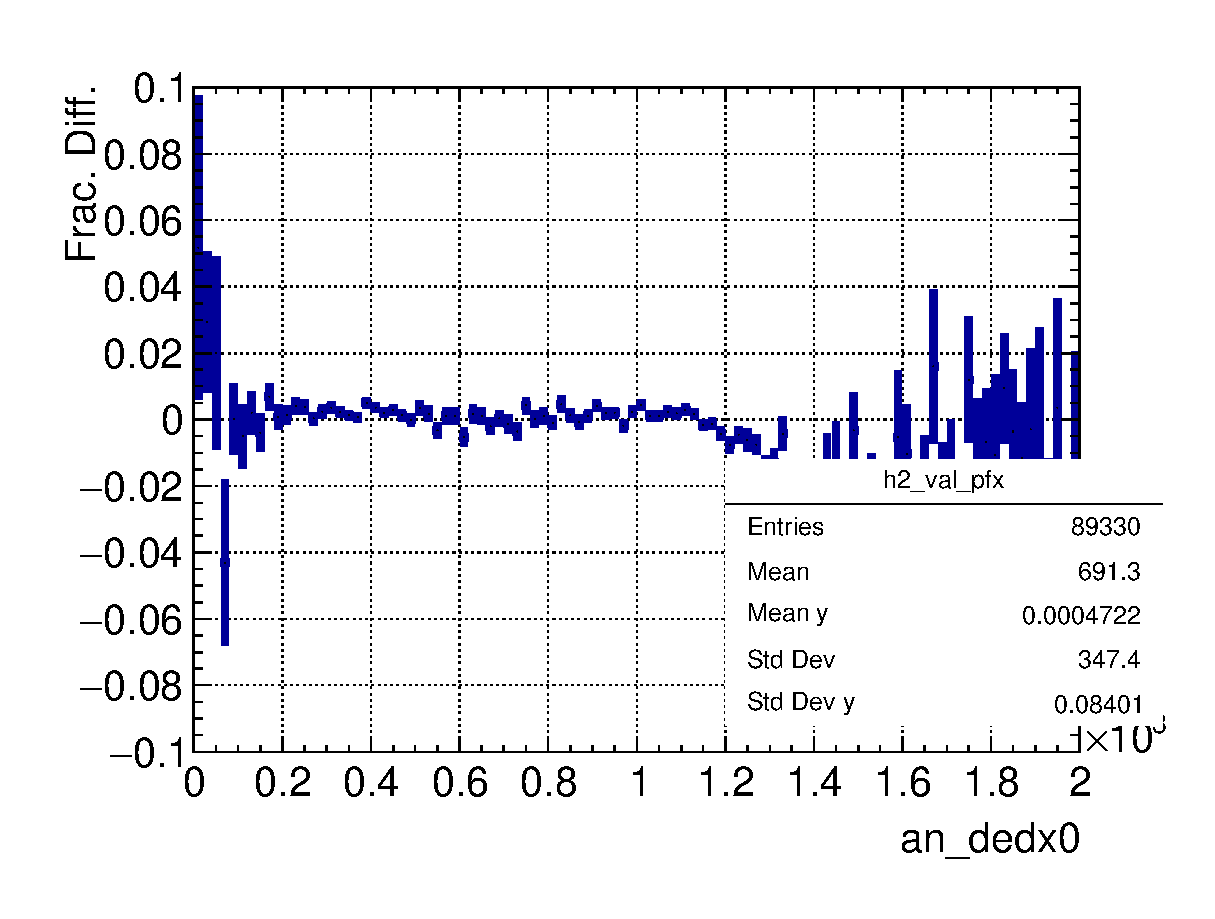
\includegraphics[width=\textwidth]{figures/sel/ans_dedx0_vs_p_pr_res_hist2d_al2_selpr_con_slice.eps}
           \caption{dedx0}
           \label{subfig:ans-dedx0-ppr-slice}
      \end{subfigure}
      \begin{subfigure}{\dbfigwid\textwidth}
           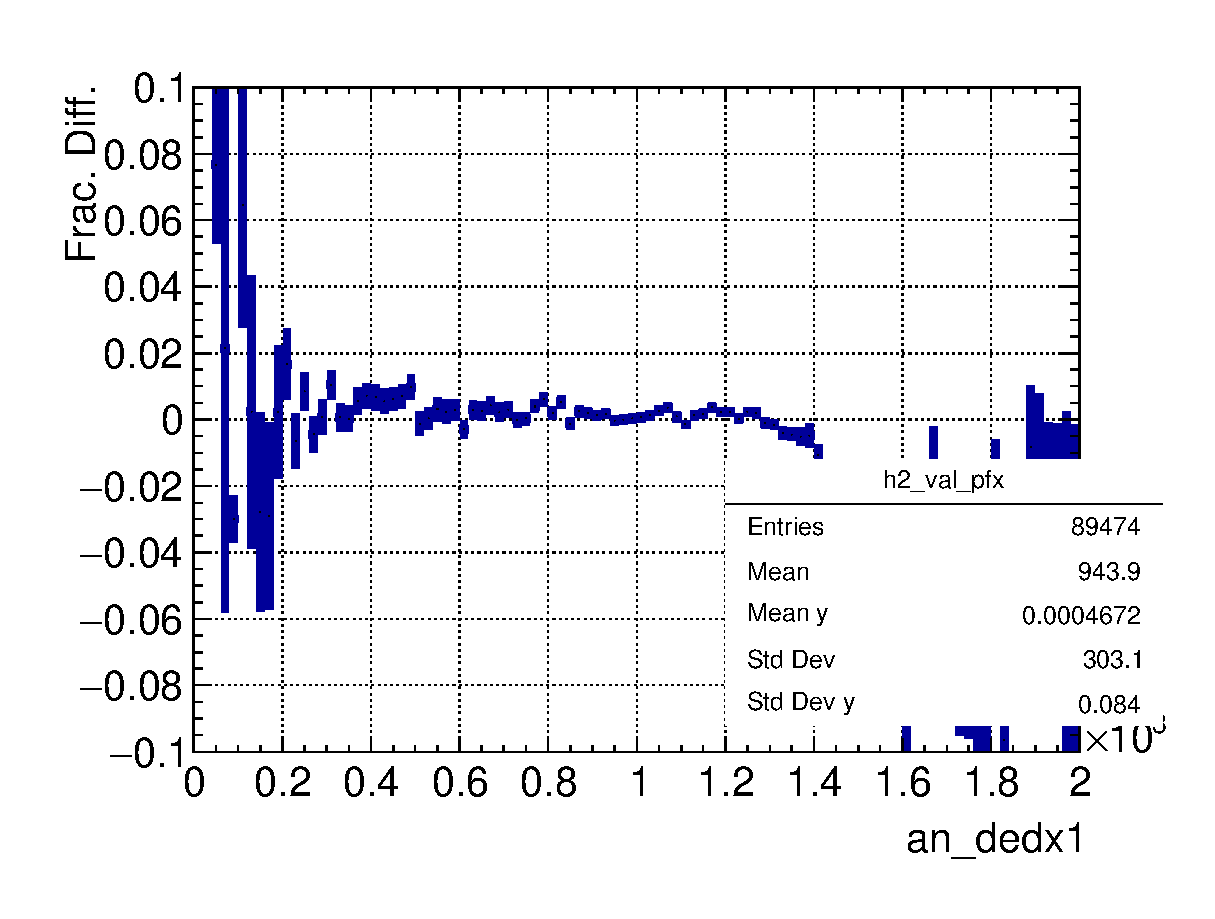
\includegraphics[width=\textwidth]{figures/sel/ans_dedx1_vs_p_pr_res_hist2d_al2_selpr_con_slice.eps}
           \caption{dedx1}
           \label{subfig:dedx1}
      \end{subfigure}
      \\
      \begin{subfigure}{\dbfigwid\textwidth}
           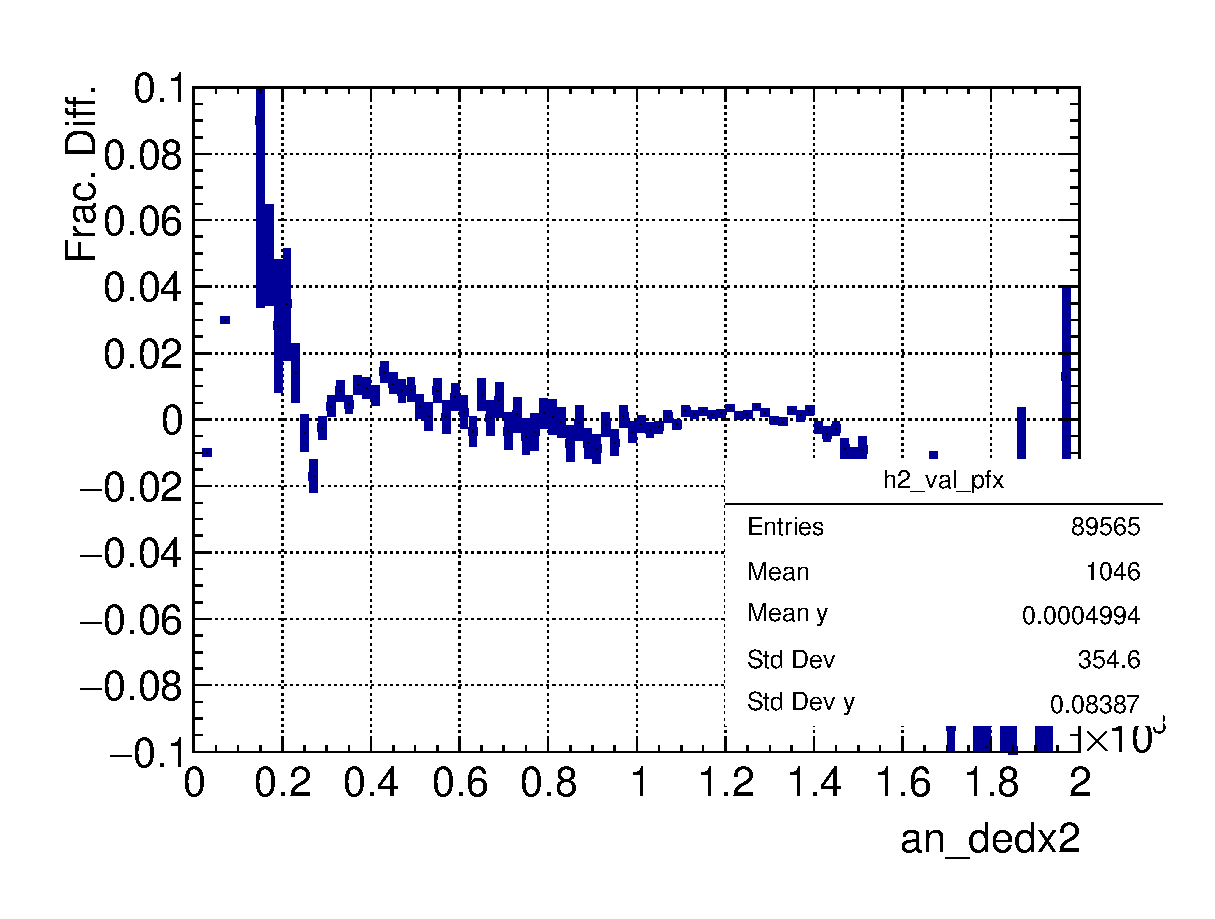
\includegraphics[width=\textwidth]{figures/sel/ans_dedx2_vs_p_pr_res_hist2d_al2_selpr_con_slice.eps}
           \caption{dedx2}
           \label{subfig:dedx2}
      \end{subfigure}
      \begin{subfigure}{\dbfigwid\textwidth}
           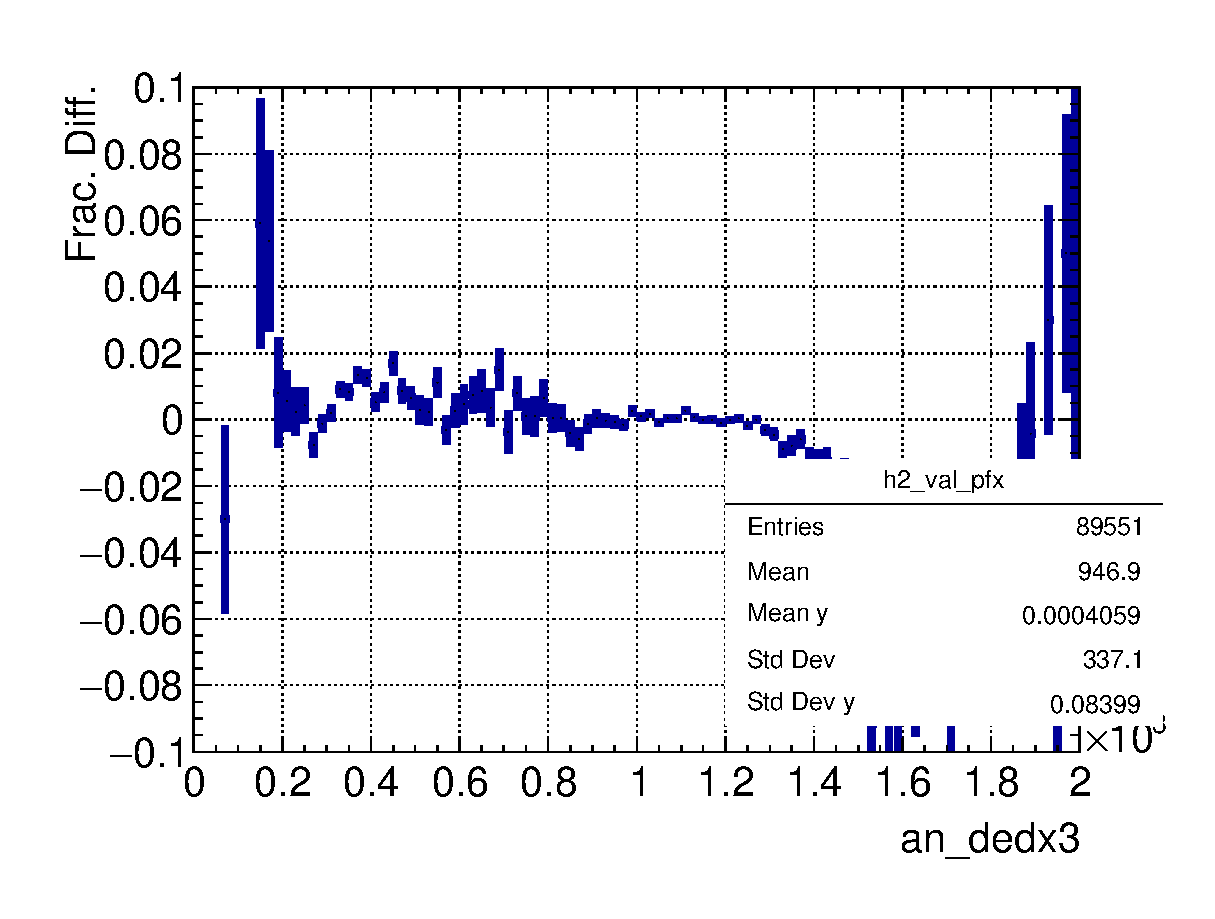
\includegraphics[width=\textwidth]{figures/sel/ans_dedx3_vs_p_pr_res_hist2d_al2_selpr_con_slice.eps}
           \caption{dedx3}
           \label{subfig:dedx3}
      \end{subfigure}
      \\
      \begin{subfigure}{\dbfigwid\textwidth}
           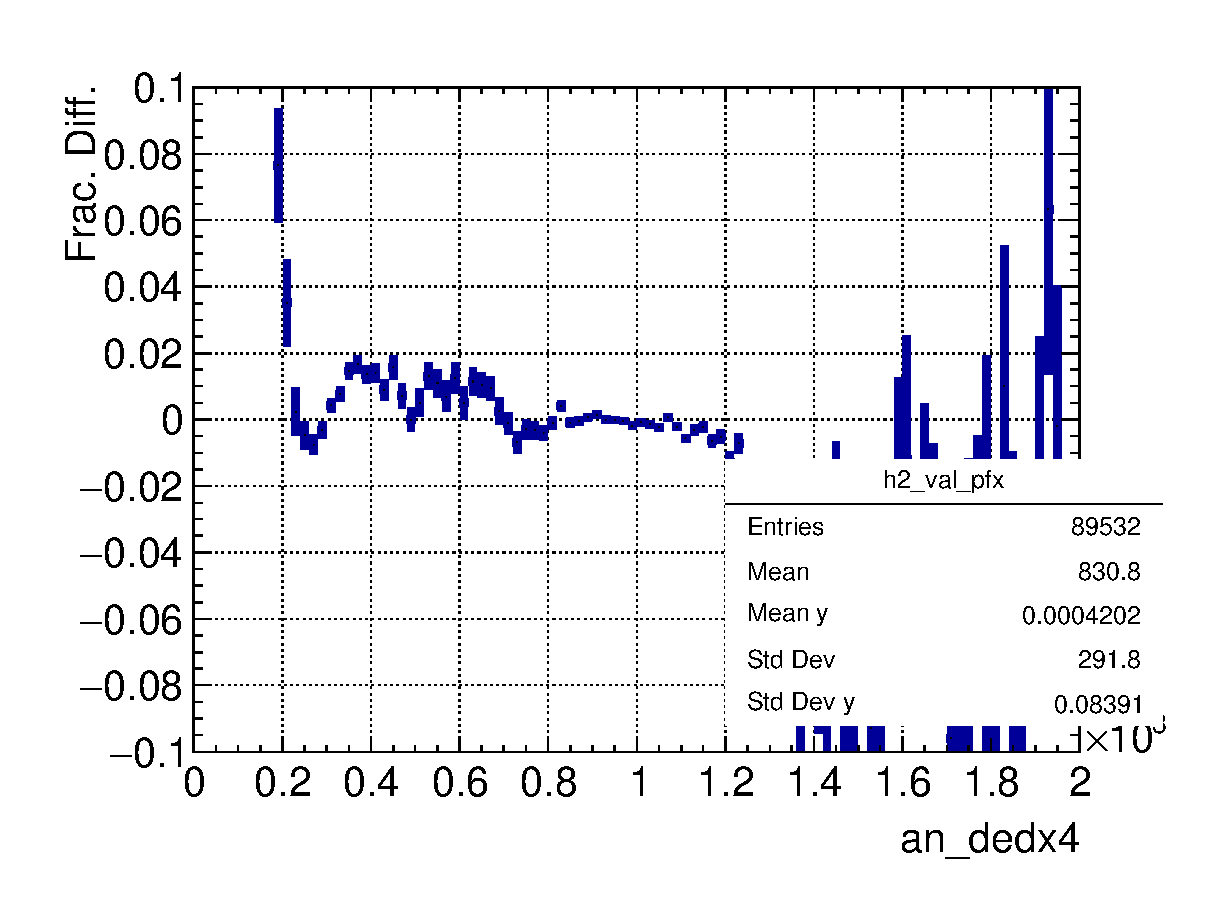
\includegraphics[width=\textwidth]{figures/sel/ans_dedx4_vs_p_pr_res_hist2d_al2_selpr_con_slice.eps}
           \caption{dedx4}
           \label{subfig:dedx4}
      \end{subfigure}
      \begin{subfigure}{\dbfigwid\textwidth}
           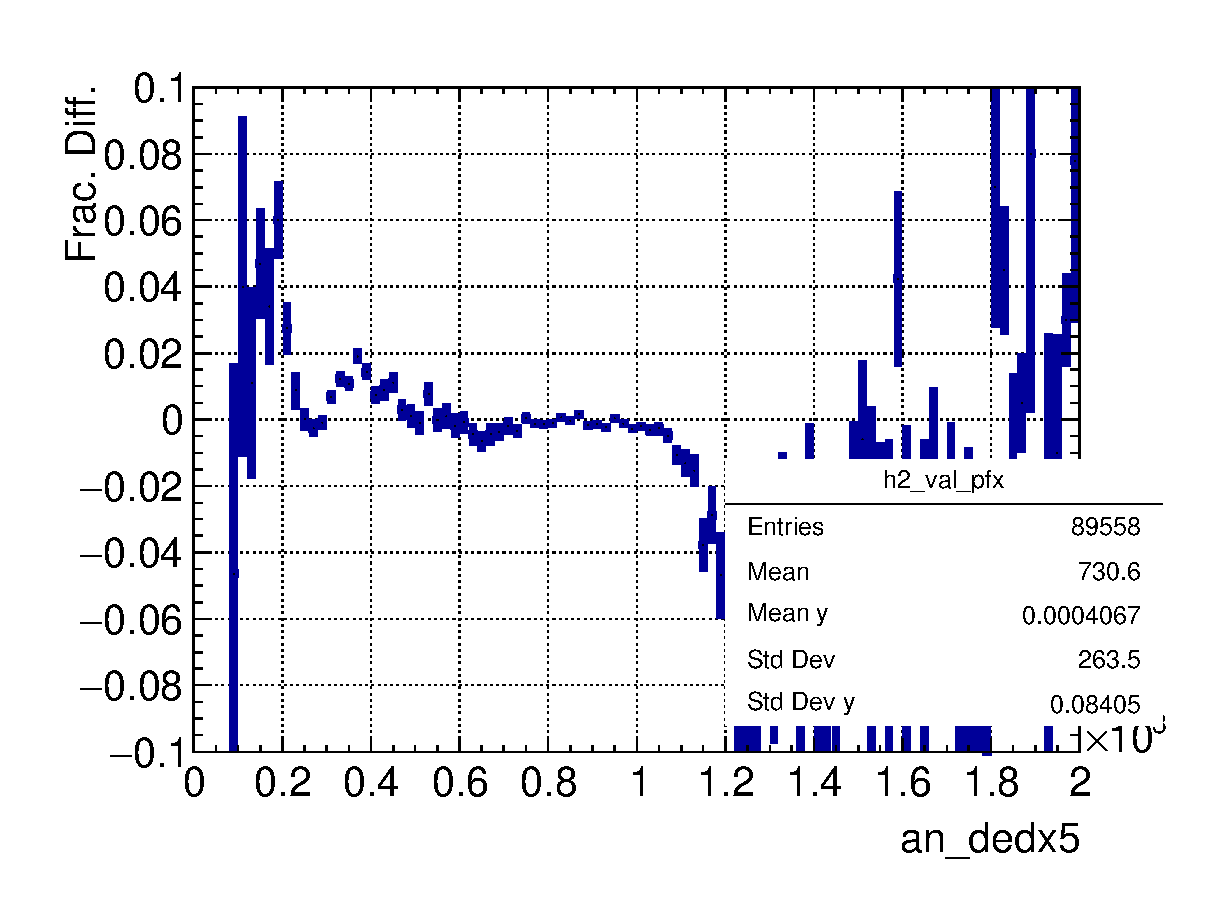
\includegraphics[width=\textwidth]{figures/sel/ans_dedx5_vs_p_pr_res_hist2d_al2_selpr_con_slice.eps}
           \caption{dedx5}
           \label{subfig:dedx5}
      \end{subfigure}
      \caption{Proton momentum reconstruction fractional difference against $\dedx$ for determination of $\dedx$ thresholds.}
      \label{fig:esc-andedx-slice}
  \end{figure}

     Furthermore, based on distributions of angle-normalized energy for the last six nodes, the average Bragg peak profile can be obtained by fitting the peaks of the distributions.
     As shown in Fig.~\ref{fig:esc-andedx-peaks}, the Bragg peak value for each node is extracted by fitting with a Cauchy function.
     From the last node backwards, the fitted Bragg peak values are $989.5$, $1080$, $1234$, $1131$, $990.0$, and $887.2$, respectively.


  \begin{figure}[t]
    \centering
    \begin{subfigure}{\dbfigwid\textwidth}
         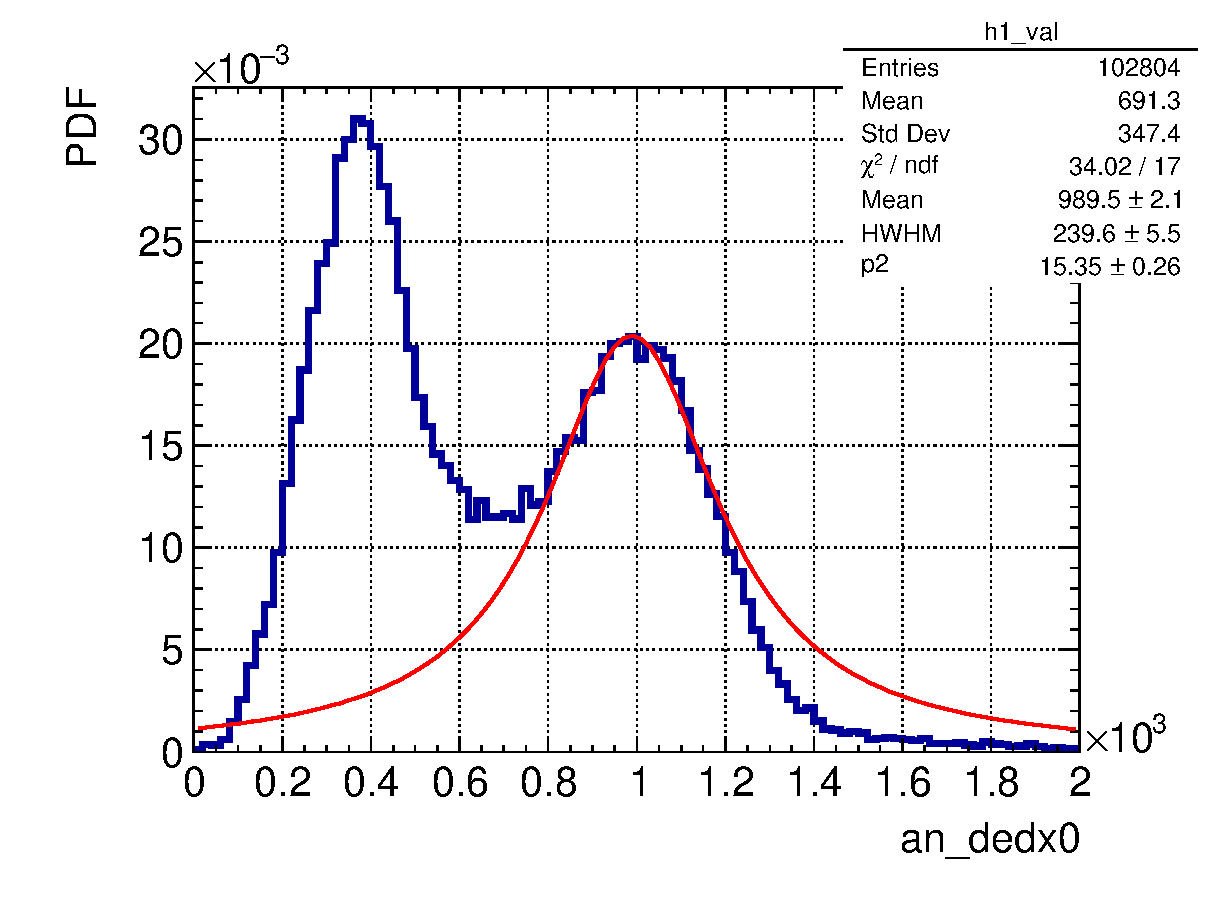
\includegraphics[width=\textwidth]{figures/sel/ans_dedx0_pdf_al2_selpr_con_test.eps}
         \caption{dedx0 peak fit}
         \label{subfig:dedx0-peak}
    \end{subfigure}
    \begin{subfigure}{\dbfigwid\textwidth}
         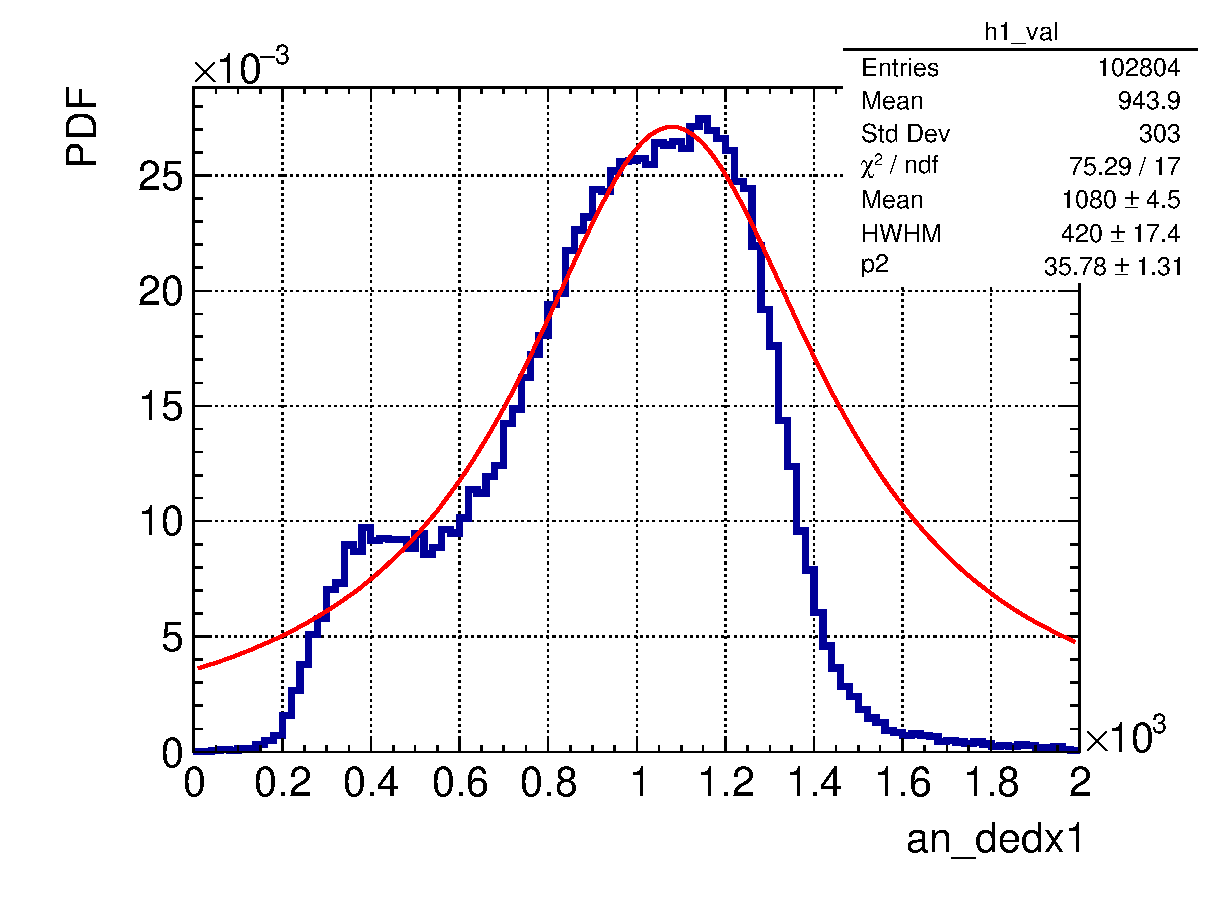
\includegraphics[width=\textwidth]{figures/sel/ans_dedx1_pdf_al2_selpr_con_test.eps}
         \caption{dedx1 peak fit}
         \label{subfig:dedx1-peak}
    \end{subfigure}
    \\
    \begin{subfigure}{\dbfigwid\textwidth}
         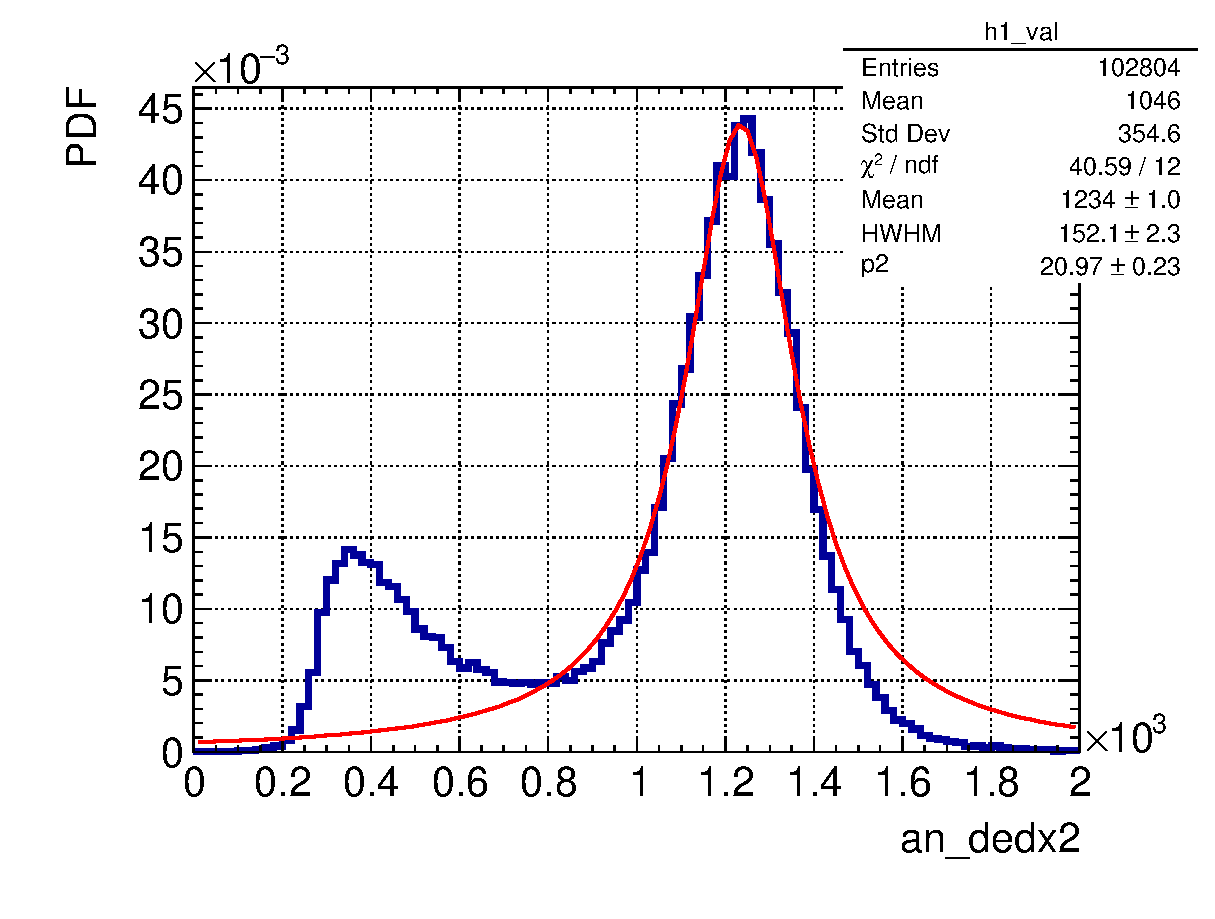
\includegraphics[width=\textwidth]{figures/sel/ans_dedx2_pdf_al2_selpr_con_test.eps}
         \caption{dedx2 peak fit}
         \label{subfig:dedx2-peak}
    \end{subfigure}
    \begin{subfigure}{\dbfigwid\textwidth}
         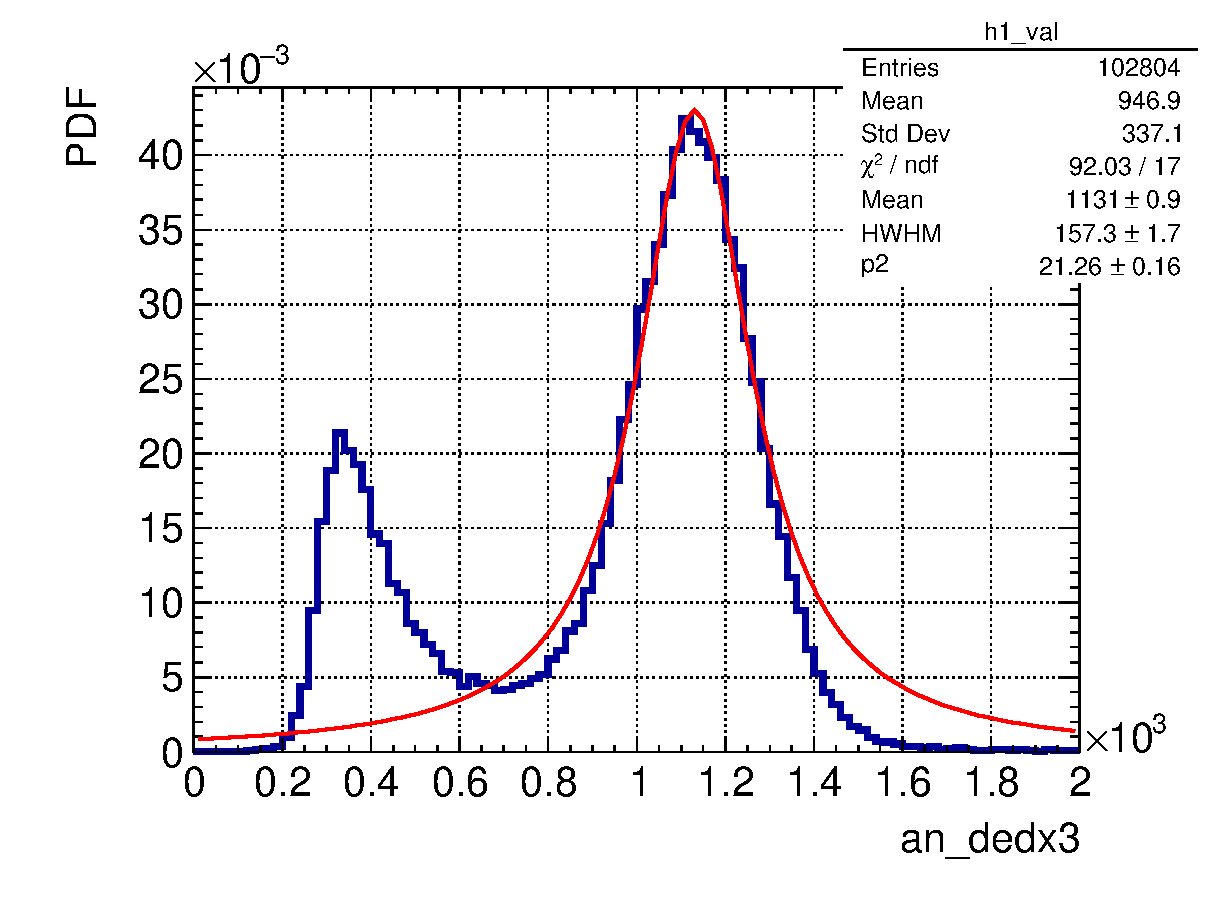
\includegraphics[width=\textwidth]{figures/sel/ans_dedx3_pdf_al2_selpr_con_test.eps}
         \caption{dedx3 peak fit}
         \label{subfig:dedx3-peak}
    \end{subfigure}
    \\
    \begin{subfigure}{\dbfigwid\textwidth}
         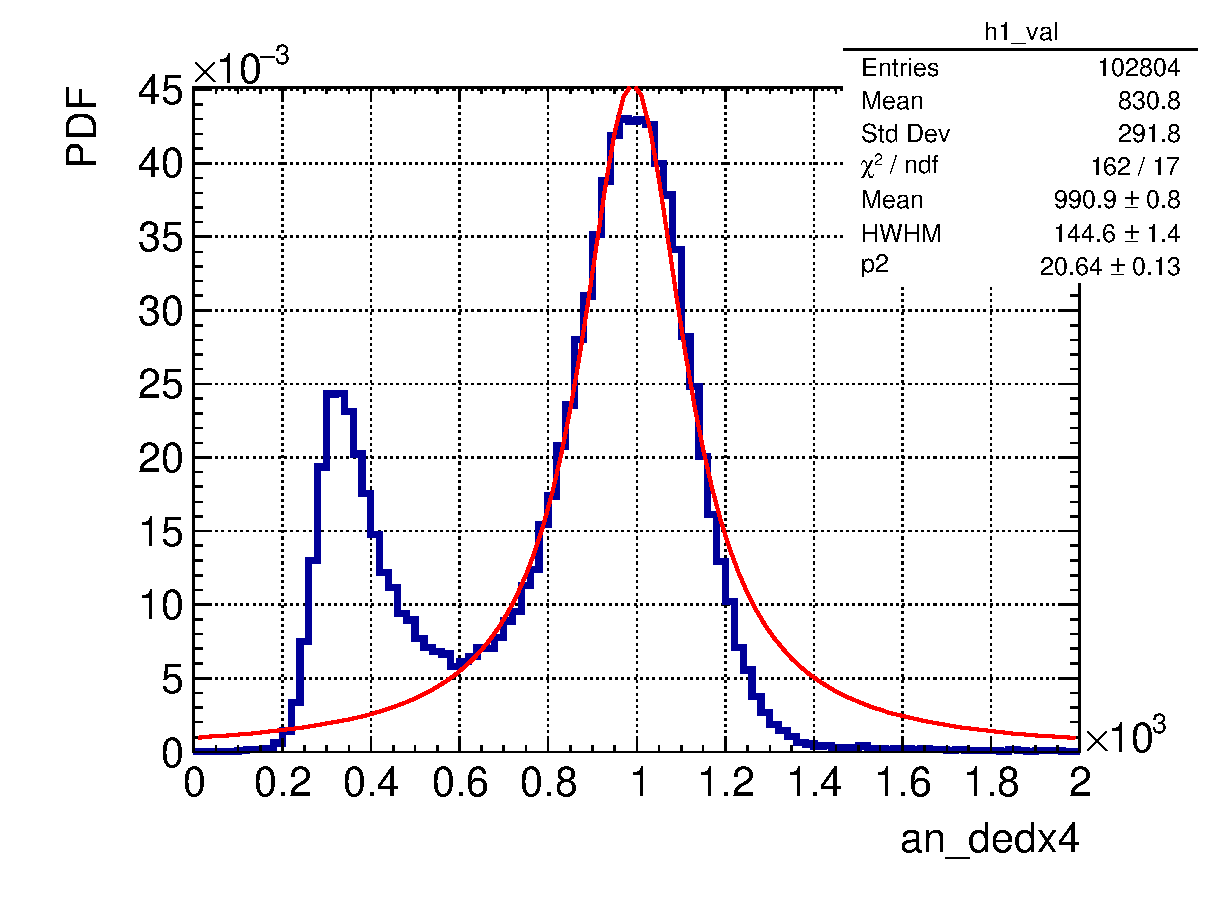
\includegraphics[width=\textwidth]{figures/sel/ans_dedx4_pdf_al2_selpr_con_test.eps}
         \caption{dedx4 peak fit}
         \label{subfig:dedx4-peak}
    \end{subfigure}
    \begin{subfigure}{\dbfigwid\textwidth}
         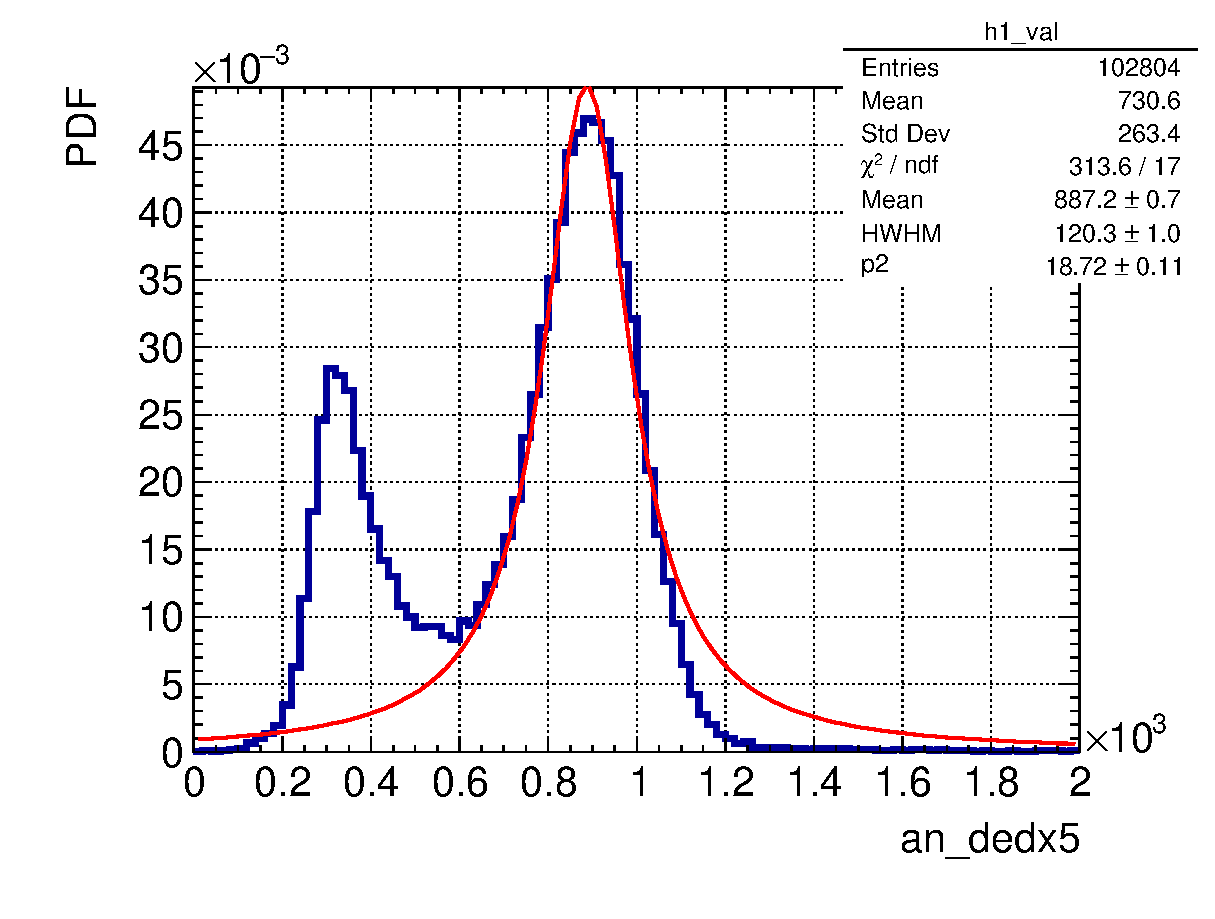
\includegraphics[width=\textwidth]{figures/sel/ans_dedx5_pdf_al2_selpr_con_test.eps}
         \caption{dedx5 peak fit}
         \label{subfig:dedx5-peak}
    \end{subfigure}
    \caption{Cauchy fits to extract the peak values of $\dedx$ at each node to estimate the average Bragg peak values.}
    \label{fig:esc-andedx-peaks}
  \end{figure}

     The angle-normalized energy for the last six nodes for each track can then be compared with this average profile using a $\chi^2$,
    \begin{equation}
    \chi^2 = \sum_{i=1}^{6} \frac{(\dedx_i - \overline{\dedx_i})^2}{\overline{\dedx_i}}
    \end{equation}
    A proton coming to rest should have a similar profile, so an upper cut on $\chi^2$ could further select protons with good momentum resolution. 
    Similar to the determination of the threshold for the individual $\dedx$, the momentum fractional difference is plotted against $\chi^2$, as shown in Fig.~\ref{fig:esc-mom-res-chi2}.
    \begin{figure}[h]
       \centering
       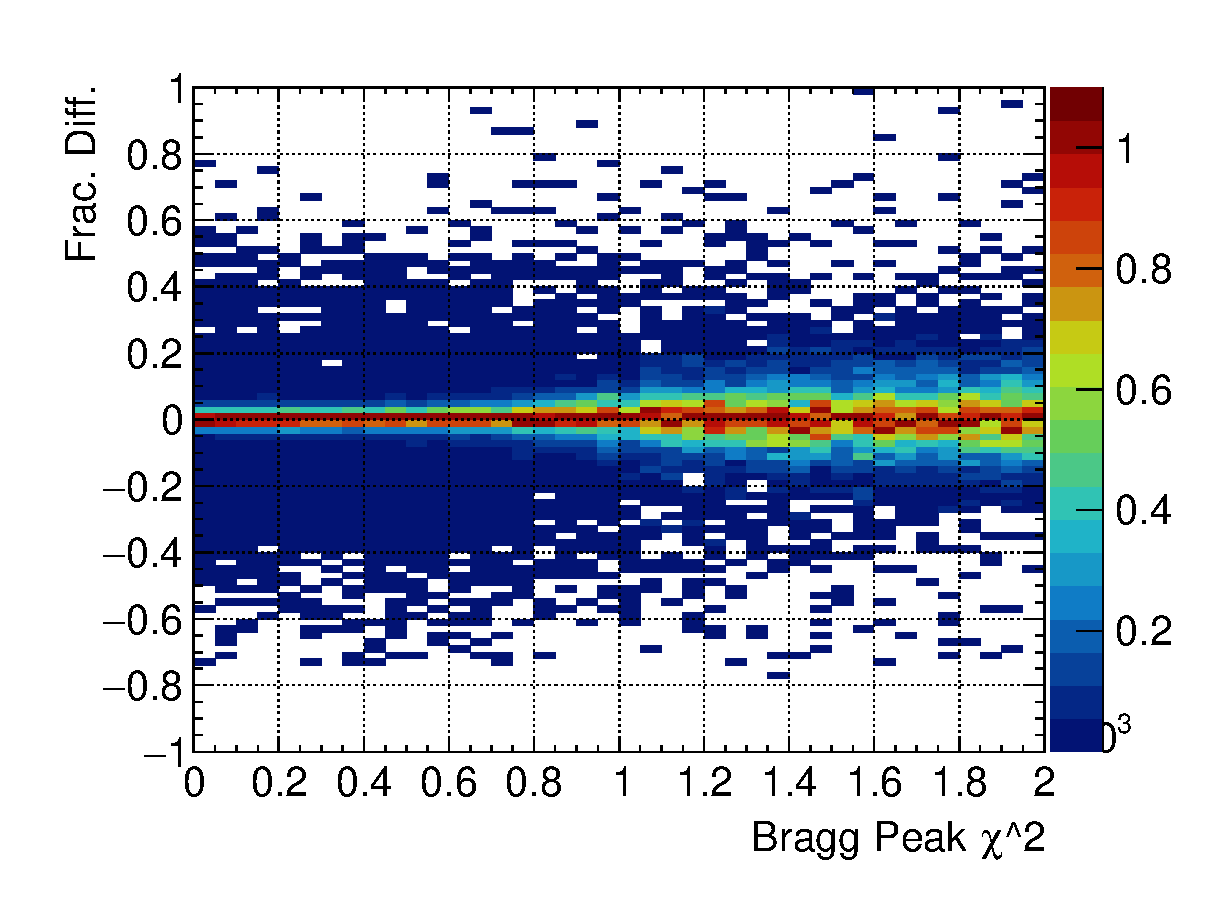
\includegraphics[width=\sgfidwid\textwidth]{figures/sel/brchi2_colnor_vs_p_pr_res_hist2d_al2_selpr_con_test.eps} 
       \caption{Proton momentum reconstruction fractional difference against $\chi^2$ for determination of $\chi^2$ thresholds.}
       \label{fig:esc-mom-res-chi2}
    \end{figure}
    The upper cut on $\chi^2$ is implemented at $800$, above which considerably larger fluctuations are observed.

    \subsection{Momentum reconstruction bias accessment}
    \label{sec:sel-esc-bias}
     In Ref.~\cite{Lu:2016mjf}, reconstruction bias in the transverse component of the momentum is observed after the ESC implementation.
     Hence, such bias is also checked for the signal sample in SFGD.
     However, unlike in Ref.~\cite{Lu:2016mjf}, no apparent bias in proton momentum reconstruction is present, while such bias is observed in muon momentum reconstruction as shown in Fig.~\ref{fig:esc-prmupt}.

     \begin{figure}
     \centering
     \begin{subfigure}[b]{\dbfigwid\textwidth}
          \centering
          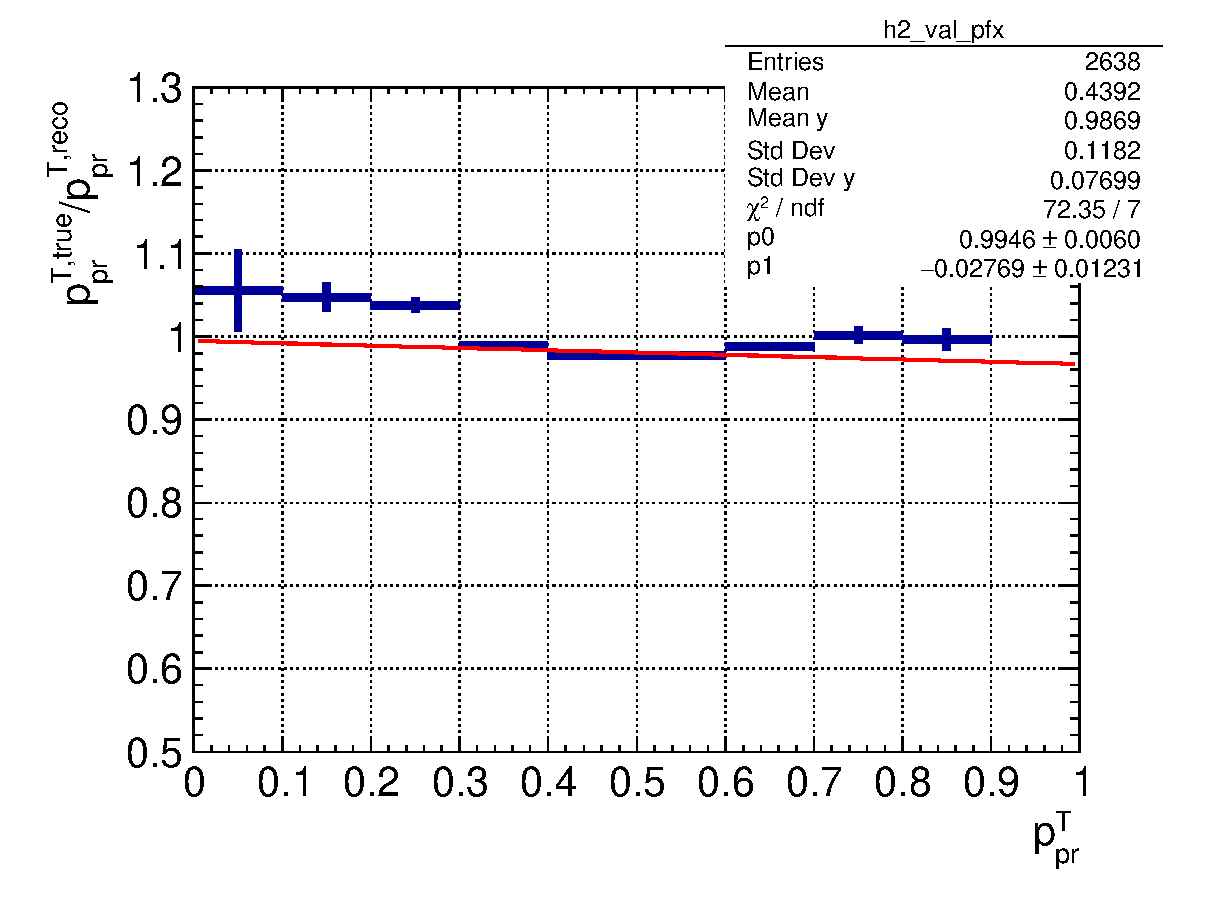
\includegraphics[width=\textwidth]{figures/sel/pr_pt_vs_pr_pt_bias_hist2d_al14.eps}
          \caption{Ratio of true$/$reco for proton $p_T$ against proton $\pt$.}
          \label{subfig:esc-prpt}
     \end{subfigure}
     \begin{subfigure}[b]{\dbfigwid\textwidth}
          \centering
          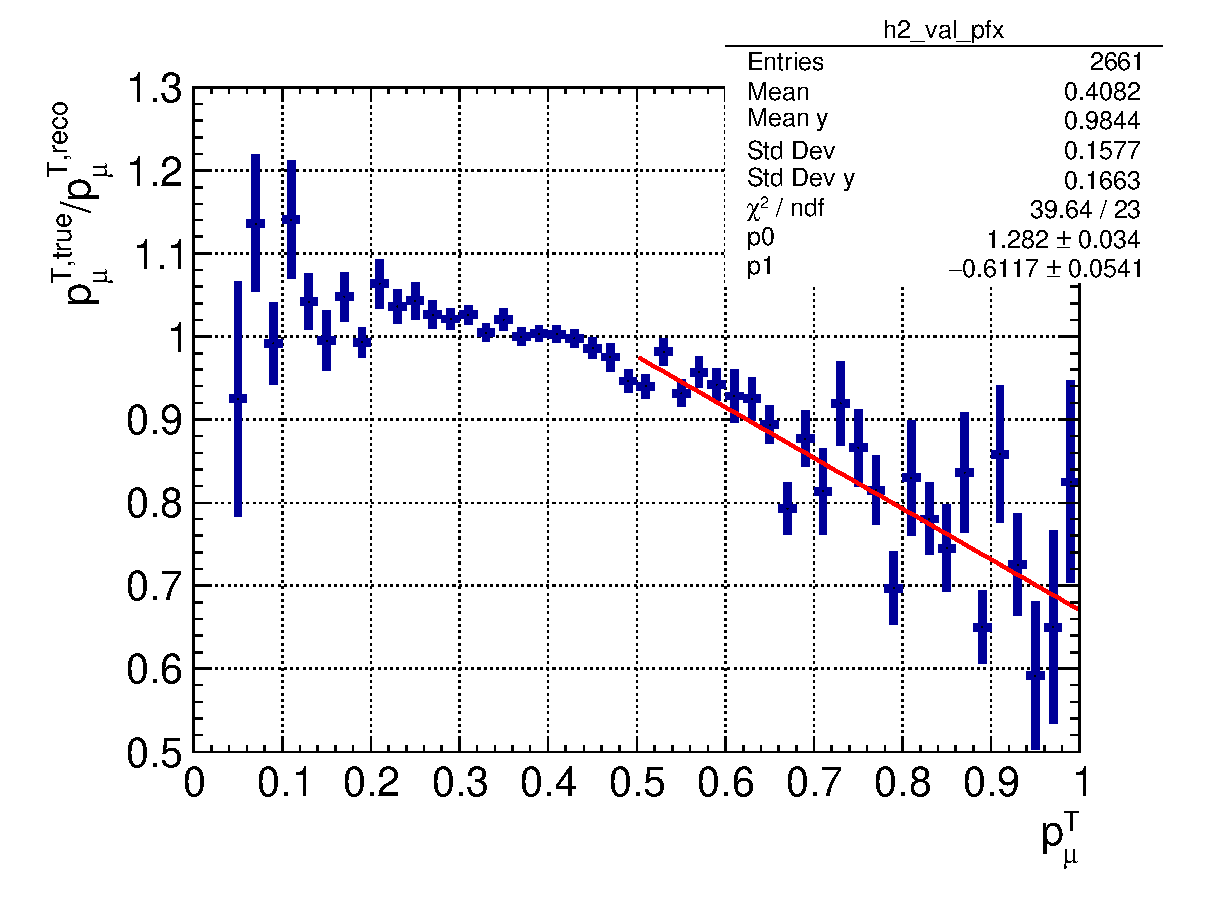
\includegraphics[width=\textwidth]{figures/sel/mu_pt_vs_mu_pt_bias_hist2d_al14.eps}
          \caption{Ratio of true$/$reco for muon $p_T$ against muon $\pt$.}
          \label{subfig:esc-mupt}
     \end{subfigure}
     \caption{Momentum Reconstruction Bias Assessment}
     \label{fig:esc-prmupt}
     \end{figure}

     Further investigation shows that there is no bias in the muon angle, as shown in Fig.~\ref{subfig:esc-mutheta}.
     Additionally, such bias is shown to be present even before the implementation of the ESC step in Fig.~\ref{subfig:esc-mupt-bfesc}, while there is no appreciable bias in the full muon momentum reconstruction.
     This could be due to a bias in the neutrino direction reconstruction.
     However, such a direction bias should have affected the proton transverse momentum as well.
     As the impact is not pronounced and the simulation software is not the final stable version yet, a correction is done solely on the muon transverse momentum for the calculations of TKI variables, and further investigations on the root cause for this bias should be carried out after a stable simulation software version becomes available.

     \begin{figure}
     \centering
     \begin{subfigure}[b]{\dbfigwid\textwidth}
          \centering
          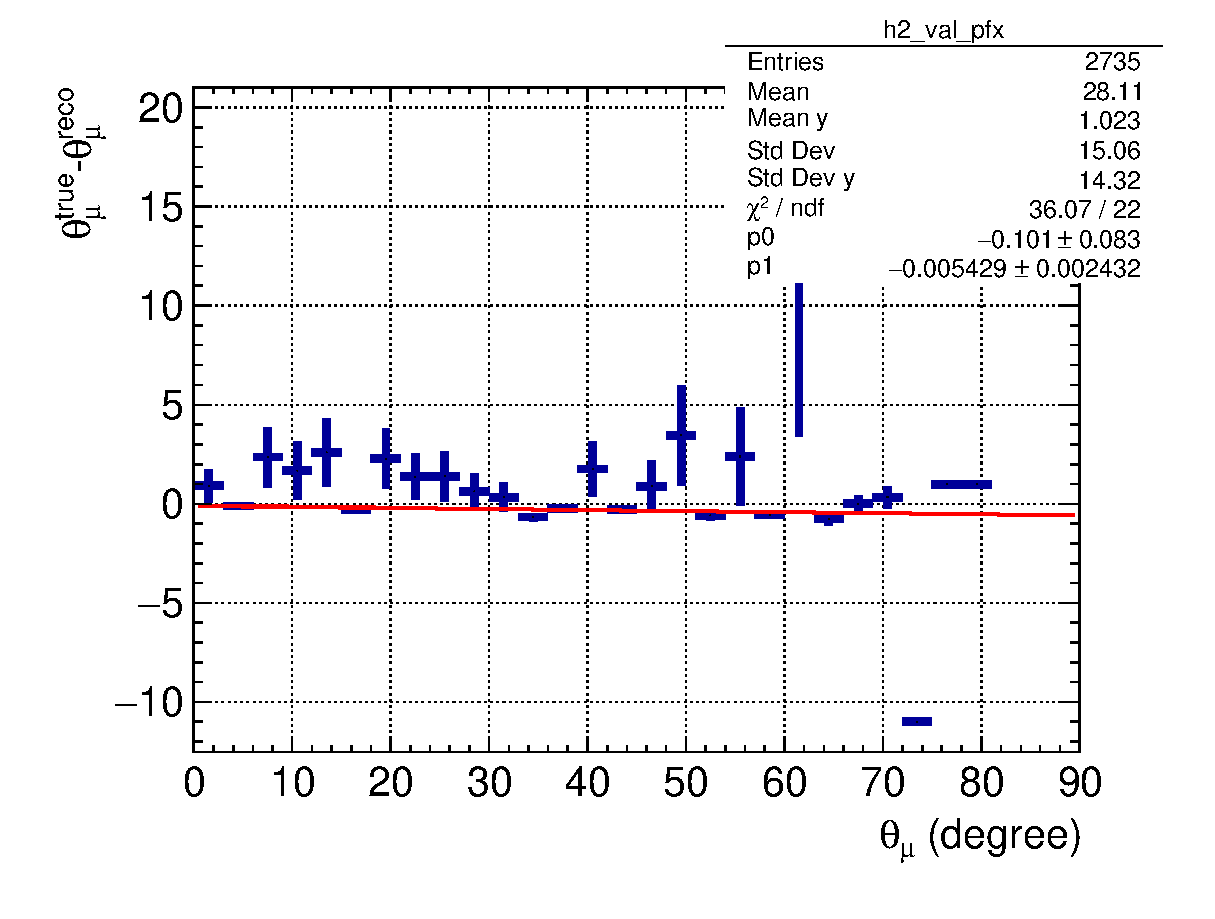
\includegraphics[width=\textwidth]{figures/sel/theta_mu_vs_theta_mu_res_hist2d_al14.eps}
          \caption{Value of true$-$reco for $\tmu$ against $\tmu$ before ESC.}
          \label{subfig:esc-mutheta}
     \end{subfigure}
     \begin{subfigure}[b]{\dbfigwid\textwidth}
          \centering
          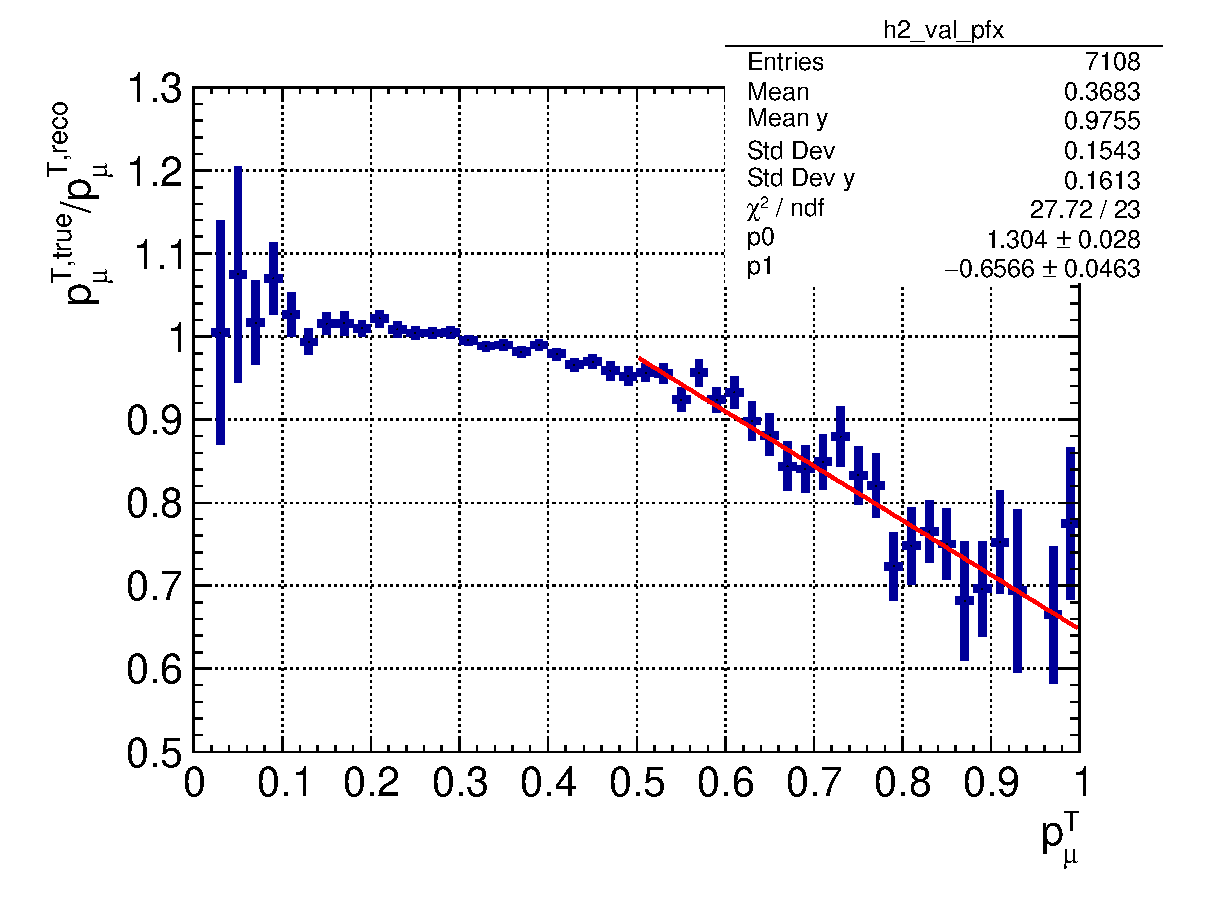
\includegraphics[width=\textwidth]{figures/sel/mu_pt_vs_mu_pt_bias_hist2d_al13.eps}
          \caption{Ratio of true$/$reco for muon $p_T$ against muon $\pt$ before ESC.}
          \label{subfig:esc-mupt-bfesc}
     \end{subfigure}
     \caption{Muon Momentum Reconstruction Bias Assessment}
     \label{fig:esc-muptcor}
     \end{figure}

     The muon correction is applied through the inverse of the linear fit of the bias region between $0.5~\gevc$ and $1.1~\gevc$.
     The corrected muon transverse momentum is shown in Fig.~\ref{fig:esc-cormupt}, which demonstrates that the bias has been rectified.

     \begin{figure}[h]
     \centering
     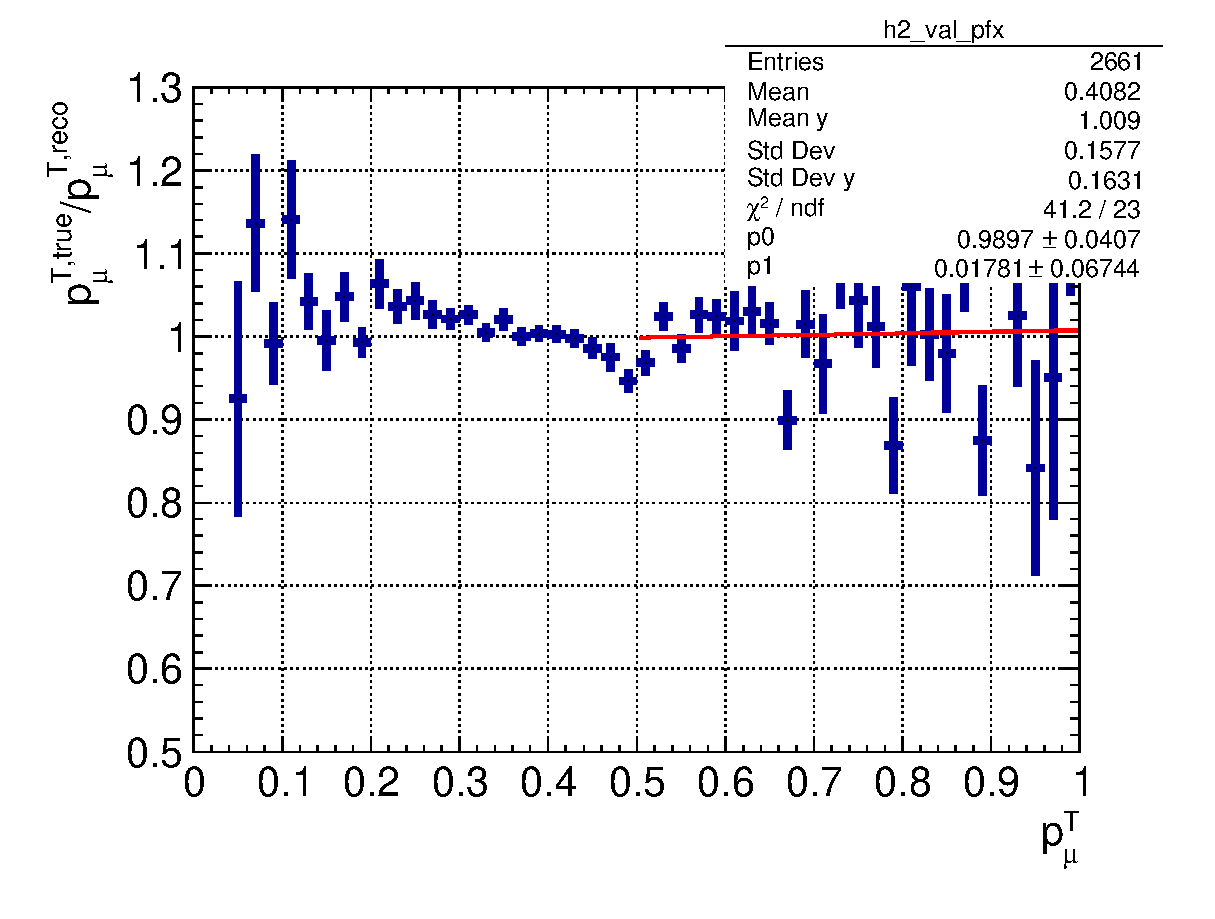
\includegraphics[width=\sgfidwid\textwidth]{figures/sel/mu_pt_vs_cor_mu_pt_bias_hist2d_al14.eps} 
     \caption{Ratio of true$/$reco for muon $p_T$ against muon $\pt$ after correction.}
     \label{fig:esc-cormupt}
     \end{figure}

    \subsection{Impacts on SPK}
     The ESC technique is completed with the transverse momentum bias correction.
     The overall impact of the technique on proton kinematics is shown in Fig.~\ref{fig:esc-spk}.
     It has significantly reduced off-diagonal entries, which represent badly reconstructed events.
     Moreover, the conspicuous line with a negative slope in the $\tpr$ has mostly disappeared.
     These could be due to a mis-reconstruction of the track direction for short protons, which are excluded by the first requirement of the ESC step: the number of nodes has to be at least $6$.
     
     \begin{figure}
        \centering
        \begin{subfigure}[b]{\dbfigwid\textwidth}
             \centering
             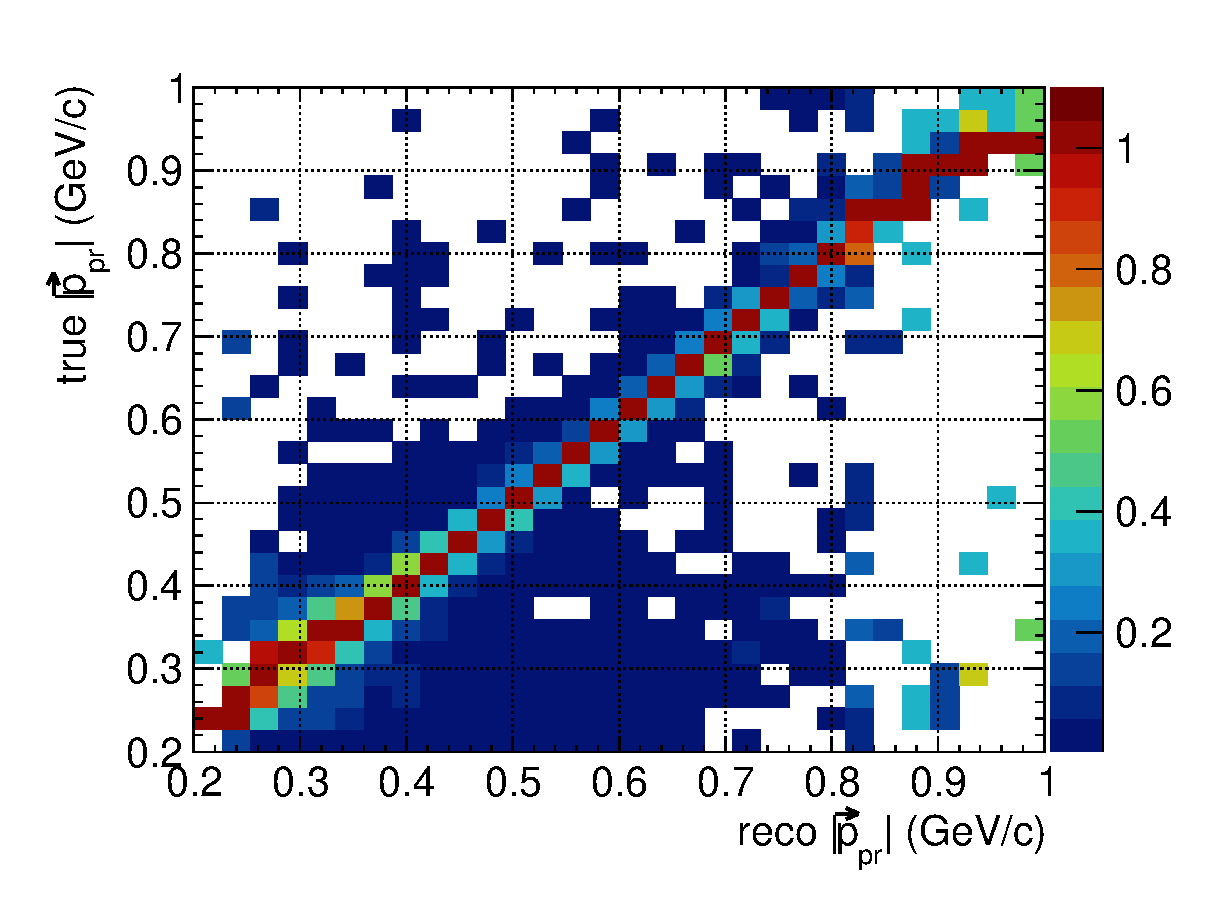
\includegraphics[width=\textwidth]{figures/sel/p_pr_colnor_resmat_al13.eps}
             \caption{$\ppr$ before ESC cut.}
             \label{subfig:esc-ppr-bfesc}
        \end{subfigure}
        \begin{subfigure}[b]{\dbfigwid\textwidth}
             \centering
             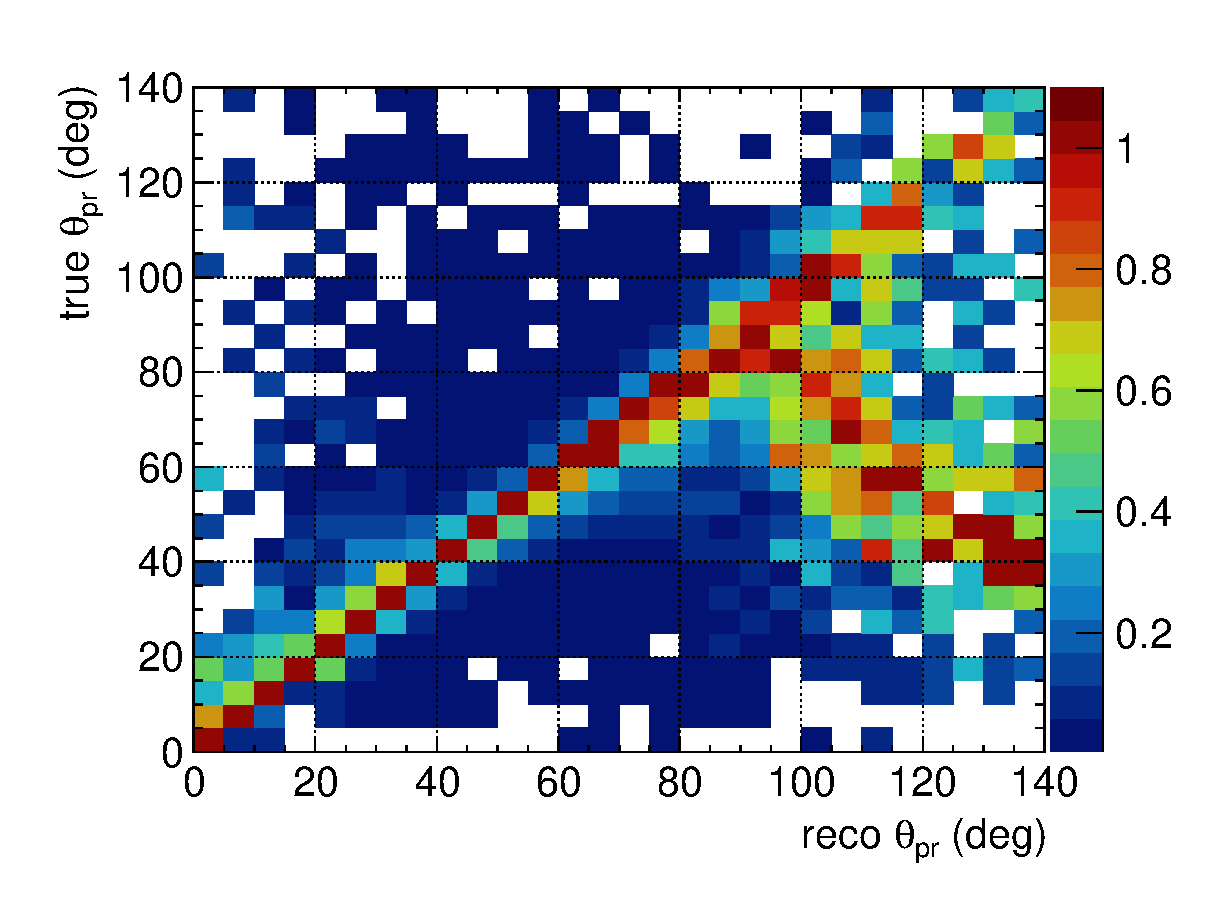
\includegraphics[width=\textwidth]{figures/sel/theta_pr_colnor_resmat_al13.eps}
             \caption{$\tpr$ before ESC cut.}
             \label{subfig:esc-tpr-bfesc}
        \end{subfigure}
        \\
        \begin{subfigure}[b]{\dbfigwid\textwidth}
             \centering
             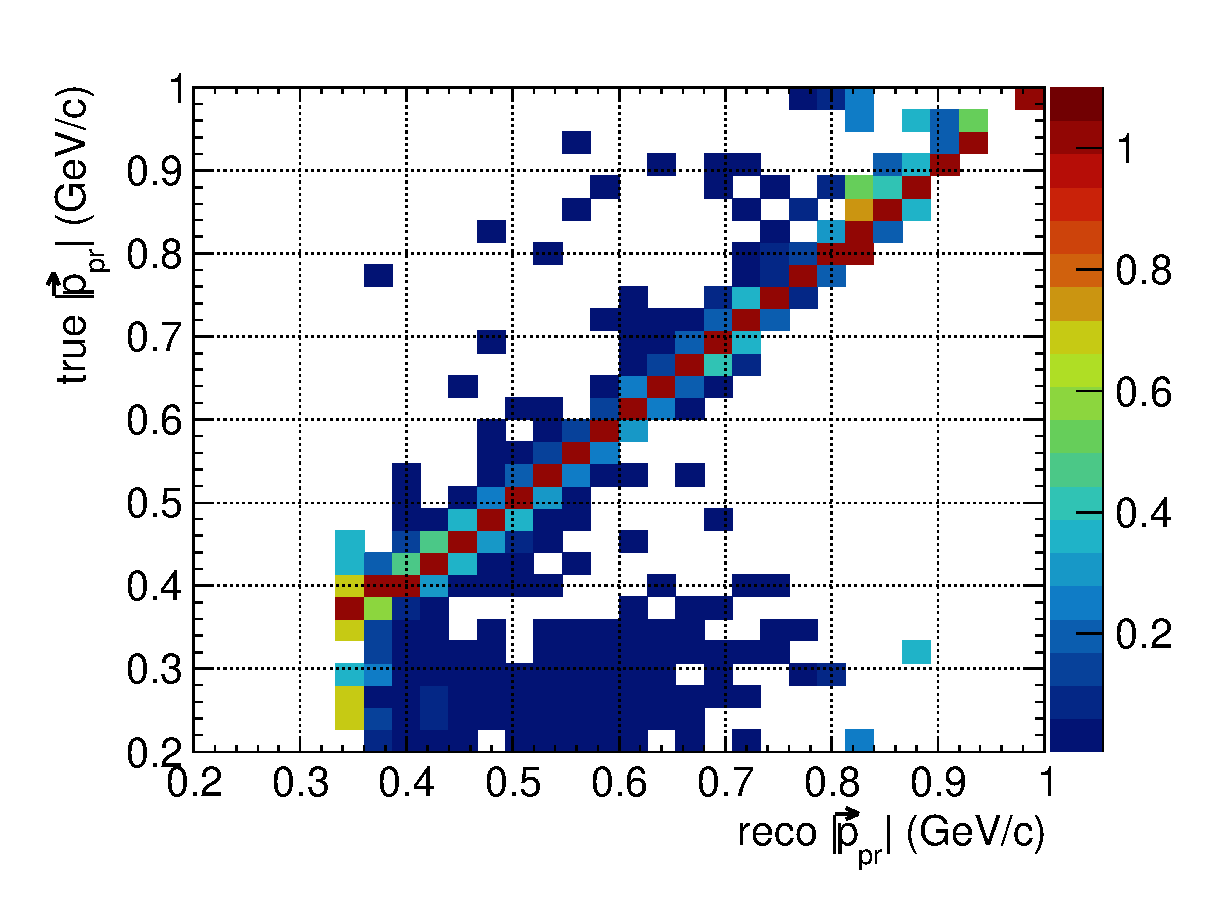
\includegraphics[width=\textwidth]{figures/sel/p_pr_colnor_resmat_al14.eps}
             \caption{$\ppr$ after ESC cut.}
             \label{subfig:esc-ppr-afesc}
        \end{subfigure}
        \begin{subfigure}[b]{\dbfigwid\textwidth}
             \centering
             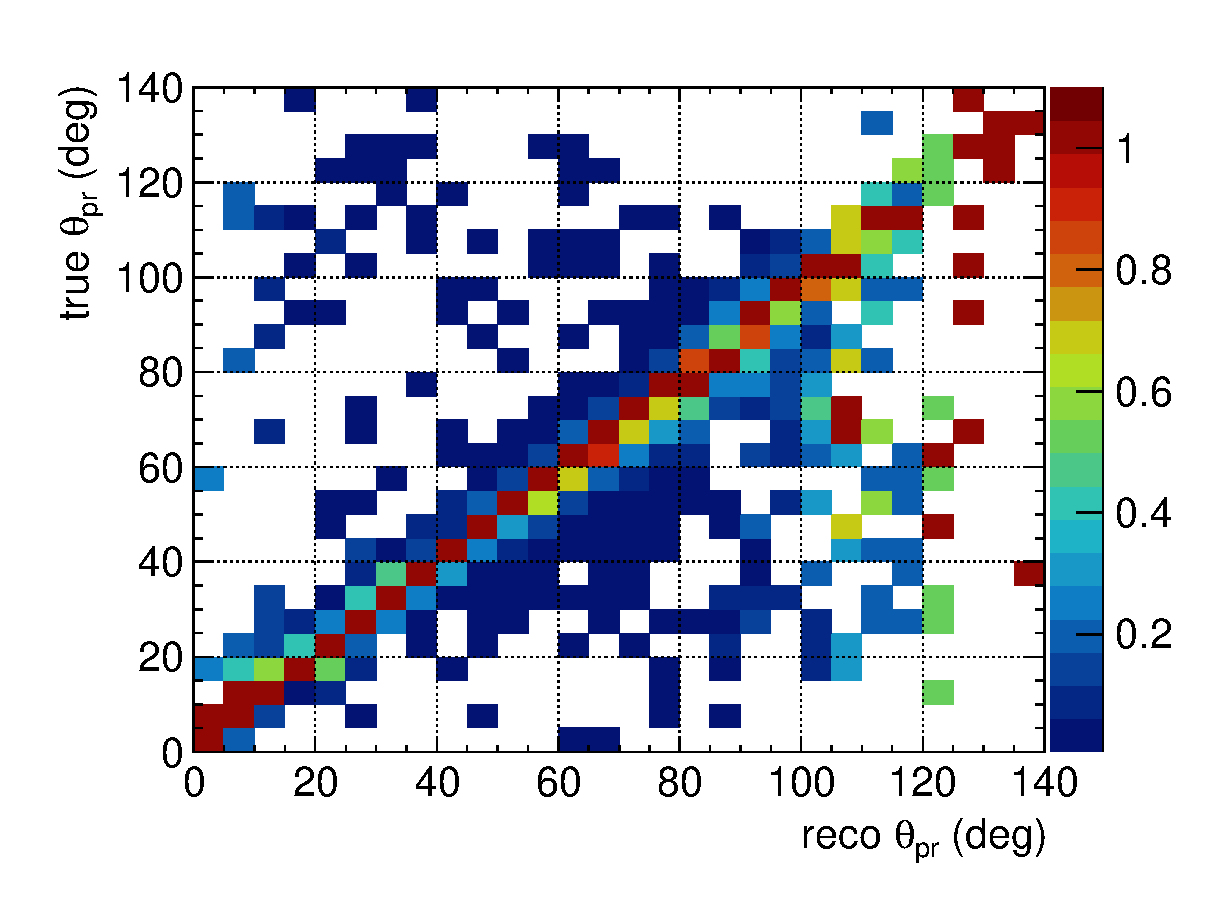
\includegraphics[width=\textwidth]{figures/sel/theta_pr_colnor_resmat_al14.eps}
             \caption{$\tpr$ after ESC cut.}
             \label{subfig:esc-tpr-afesc}
        \end{subfigure}
        \caption{SPK before and after ESC.}
        \label{fig:esc-spk}
  \end{figure}

     The overall improvement in the SPK is best illustrated with a Cauchy fit to the proton momentum reconstruction resolution histogram, as shown in Fig.~\ref{subfig:ppr-res-bfESC} and Fig.~\ref{subfig:ppr-res-afESC}, which shows a more than $50\%$ reduction in the width of the distribution.
     This improvement is achieved at the cost of a two-thirds reduction in efficiency, as shown in Fig.~\ref{subfig:ppr-eff-bfESC} and Fig.~\ref{subfig:ppr-eff-afESC}.
     The drop in efficiency might seem drastic, but it proves to be necessary for the TKI analysis, as shown later in Sec.~\ref{sec:mc-tki}, which showcases the significant improvement in the evaluation of TKI variables due to the ESC technique.

   \begin{figure}[t]
      \centering
      \begin{subfigure}{\dbfigwid\textwidth}
           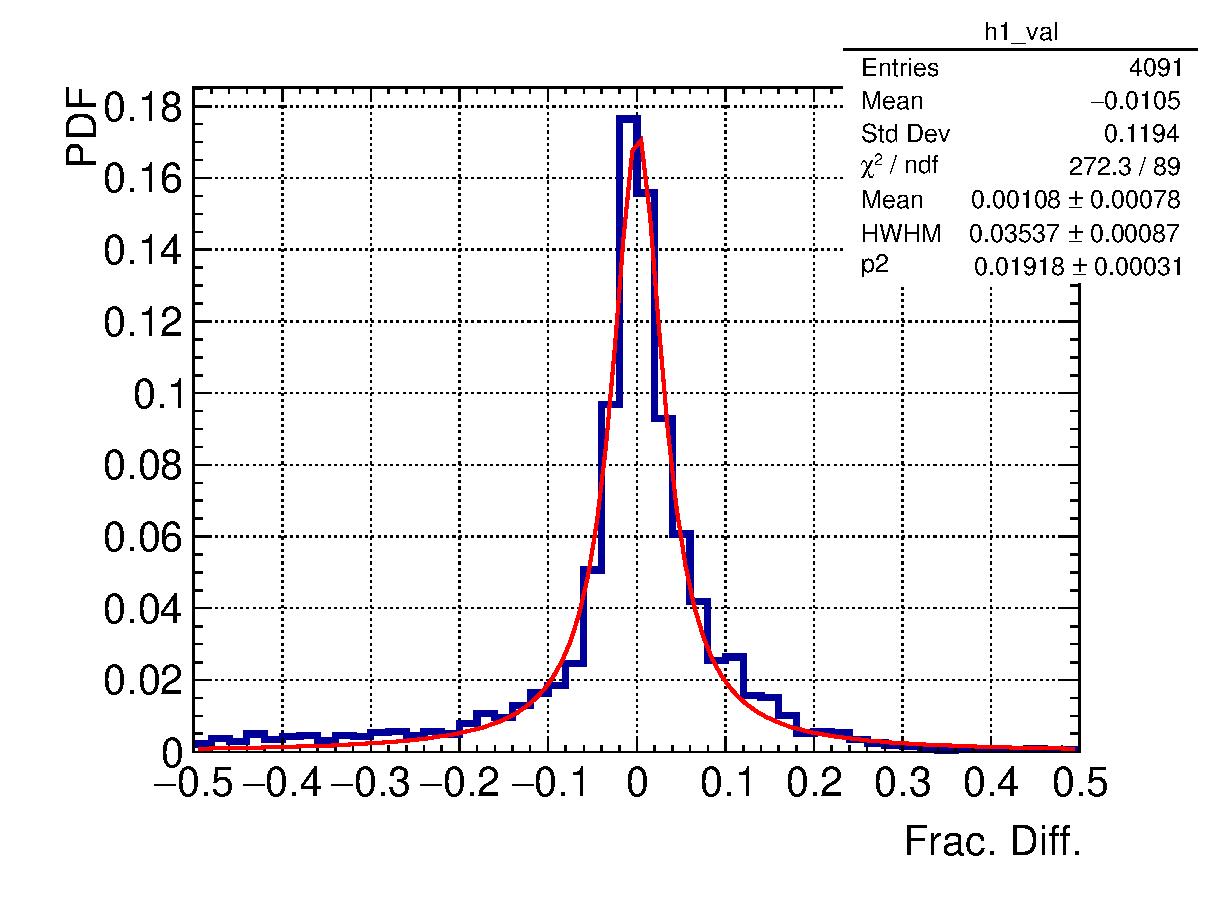
\includegraphics[width=\textwidth]{figures/sel/p_pr_res_pdf_al13_zoom.eps}
           \caption{$\pp$ resolution before ESC selection. The fitted half width is about $3.5\%$.}
           \label{subfig:ppr-res-bfESC}
      \end{subfigure}
      \begin{subfigure}{\dbfigwid\textwidth}
           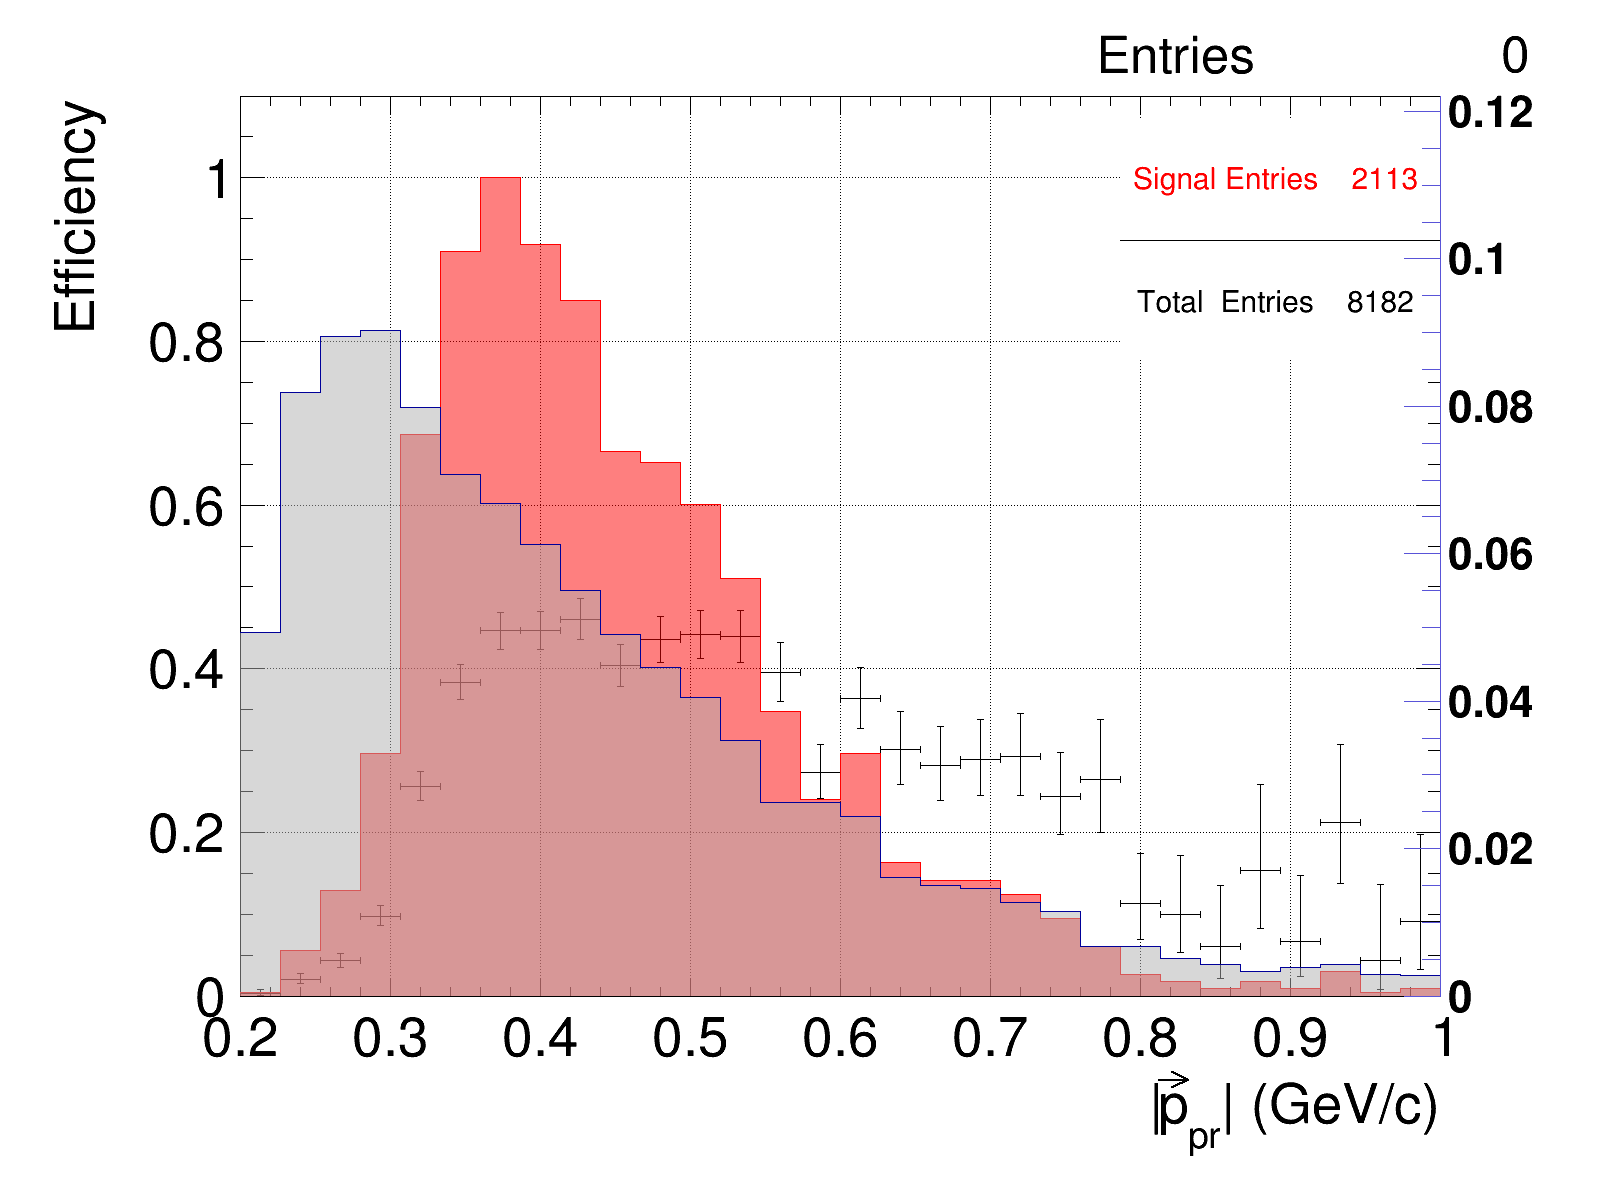
\includegraphics[width=\textwidth]{figures/sel/p_pr_eff_al13.png}
           \caption{Selection efficiency before ESC selection. The overall efficiency is $2113/8182\approx25.8\%$.}
           \label{subfig:ppr-eff-bfESC}
      \end{subfigure}
      \\
      \begin{subfigure}{\dbfigwid\textwidth}
           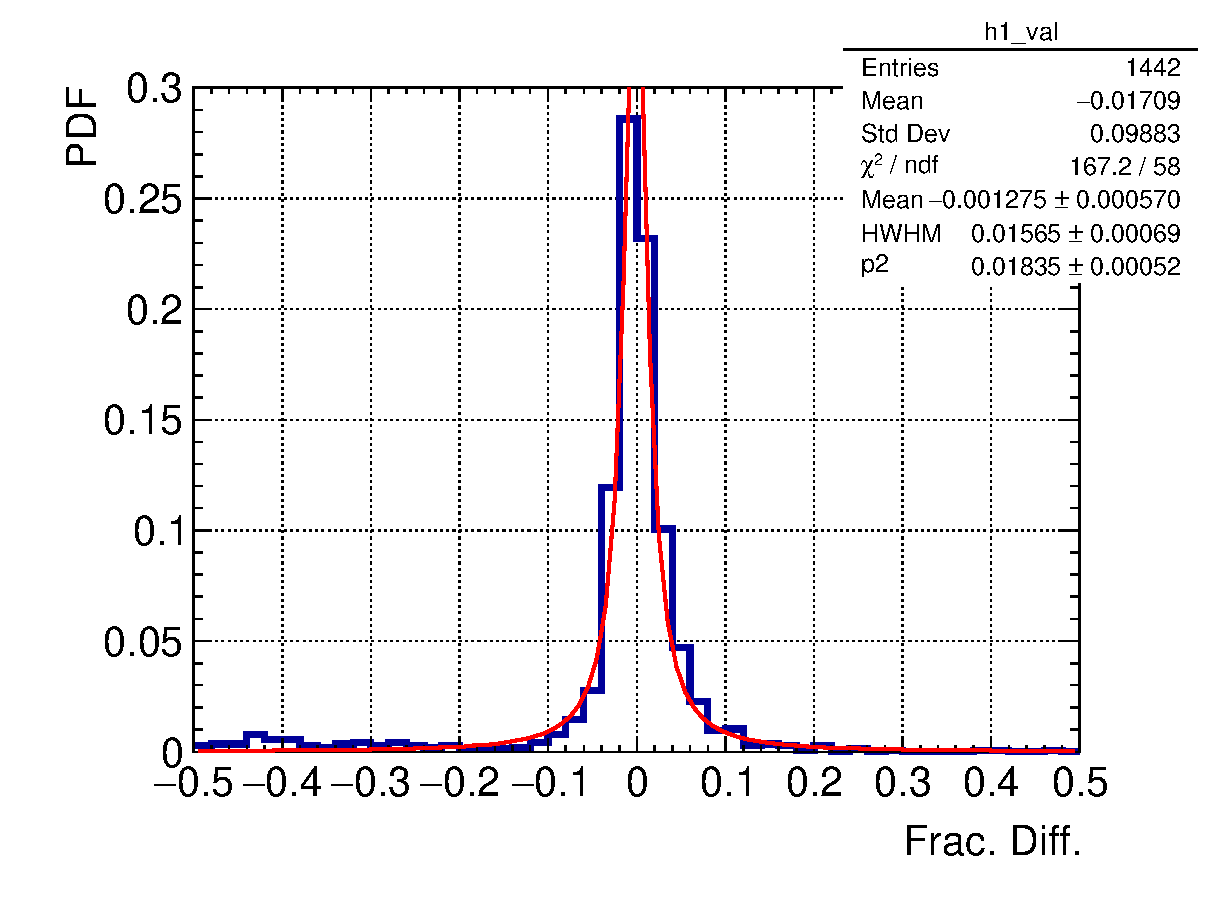
\includegraphics[width=\textwidth]{figures/sel/p_pr_res_pdf_al14_zoom.eps}
           \caption{$\ppr$ resolution after ESC selection. The fitted half width is about $1.6\%$.}
           \label{subfig:ppr-res-afESC}
      \end{subfigure}
      \begin{subfigure}{\dbfigwid\textwidth}
           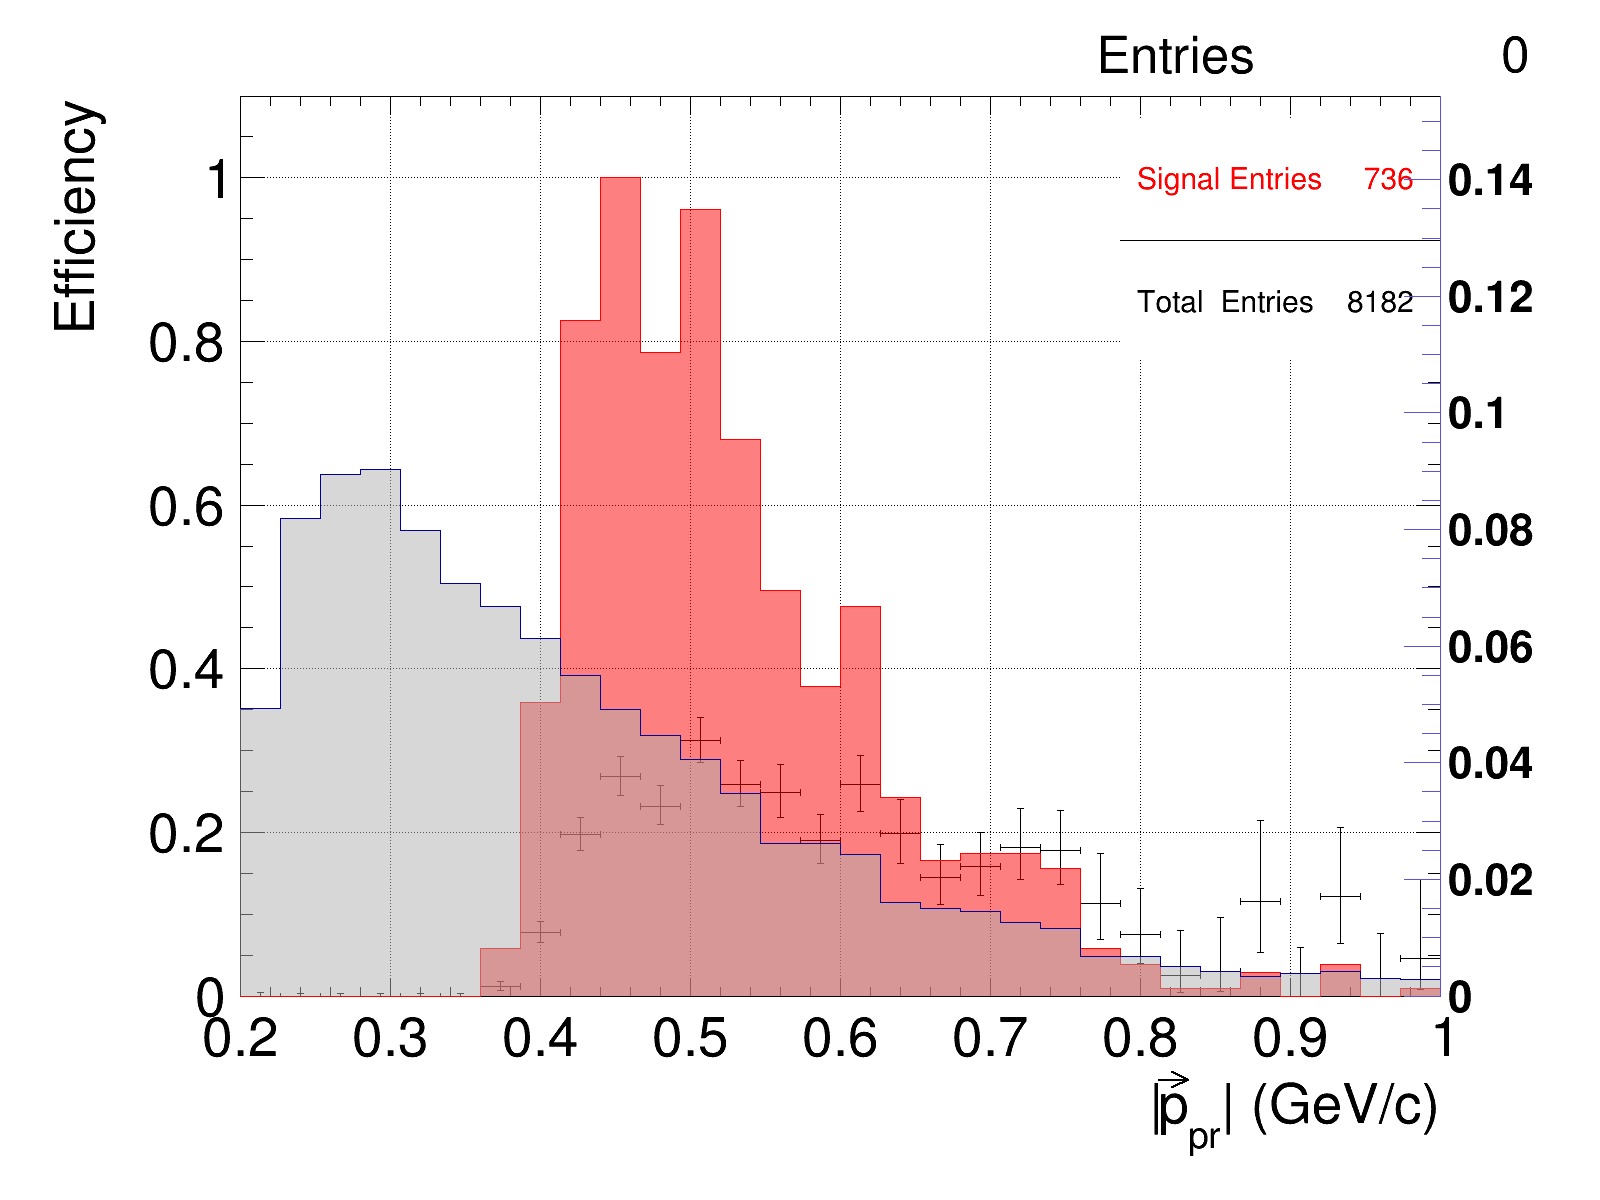
\includegraphics[width=\textwidth]{figures/sel/p_pr_eff_al14.png}
           \caption{Selection efficiency after ESC selection. The overall efficiency is $736/8182\approx9.0\%$}
           \label{subfig:ppr-eff-afESC}
      \end{subfigure}
      \caption{Proton ESC selection results. The grey histograms are the true probability distribution, while the pink ones are those that get reconstructed. }
      \label{fig:esc-ppr-reseff}
   \end{figure}


    %------------------- pion TL ----------------%
    \section{Pion Trackless Reconstruction}
       \label{sec:sel-tl}
          As briefly elaborated in Sec.~\ref{sec:t2k-sw}, in SFGD, particle identification and momentum reconstruction are only performed on reconstructed tracks, which have a minimum length of about $30$~mm. 
          Hence, low-momentum particles, which travel only a short distance, could not be reconstructed at all. 
          When these low-momentum pions are not reconstructed, these $\ccopi$ events are misidentified as $\cczpi$ events, both decreasing the signal for the $\ccopi$ samples and increasing the background for the $\cczpi$ sample. 
          Thus, it would be highly beneficial if we could reconstruct these pions. 
          The pion trackless reconstruction technique I have developed can address this gap perfectly.

     
       \subsection{preliminary Study}
       \label{sec:tl-ps}
          Before developing the pion trackless reconstruction technique, it is essential to assess its potential significance, as this technique can only reconstruct pions that decay at rest. 
          If only a limited number of pions decay in this manner, the technique would be inapplicable. 
          Therefore, a preliminary study on pion fates relevant to T2K was conducted.

          The first step involved examining the primary pion momentum distribution in SFGD as produced by the T2K flux. 
          For a rough estimation, the first 100,000 events in the T2K input flux file were processed through the T2K ND simulation, and events containing a primary pion were recorded. 
          The true pion momentum cumulative distribution is shown in Fig.~\ref{subfig:pi-mom-cum}, indicating that the majority of pions have momentum below $1000~\mevc$.

          \begin{figure}[t]
               \centering
               \begin{subfigure}{\dbfigwid\textwidth}
                    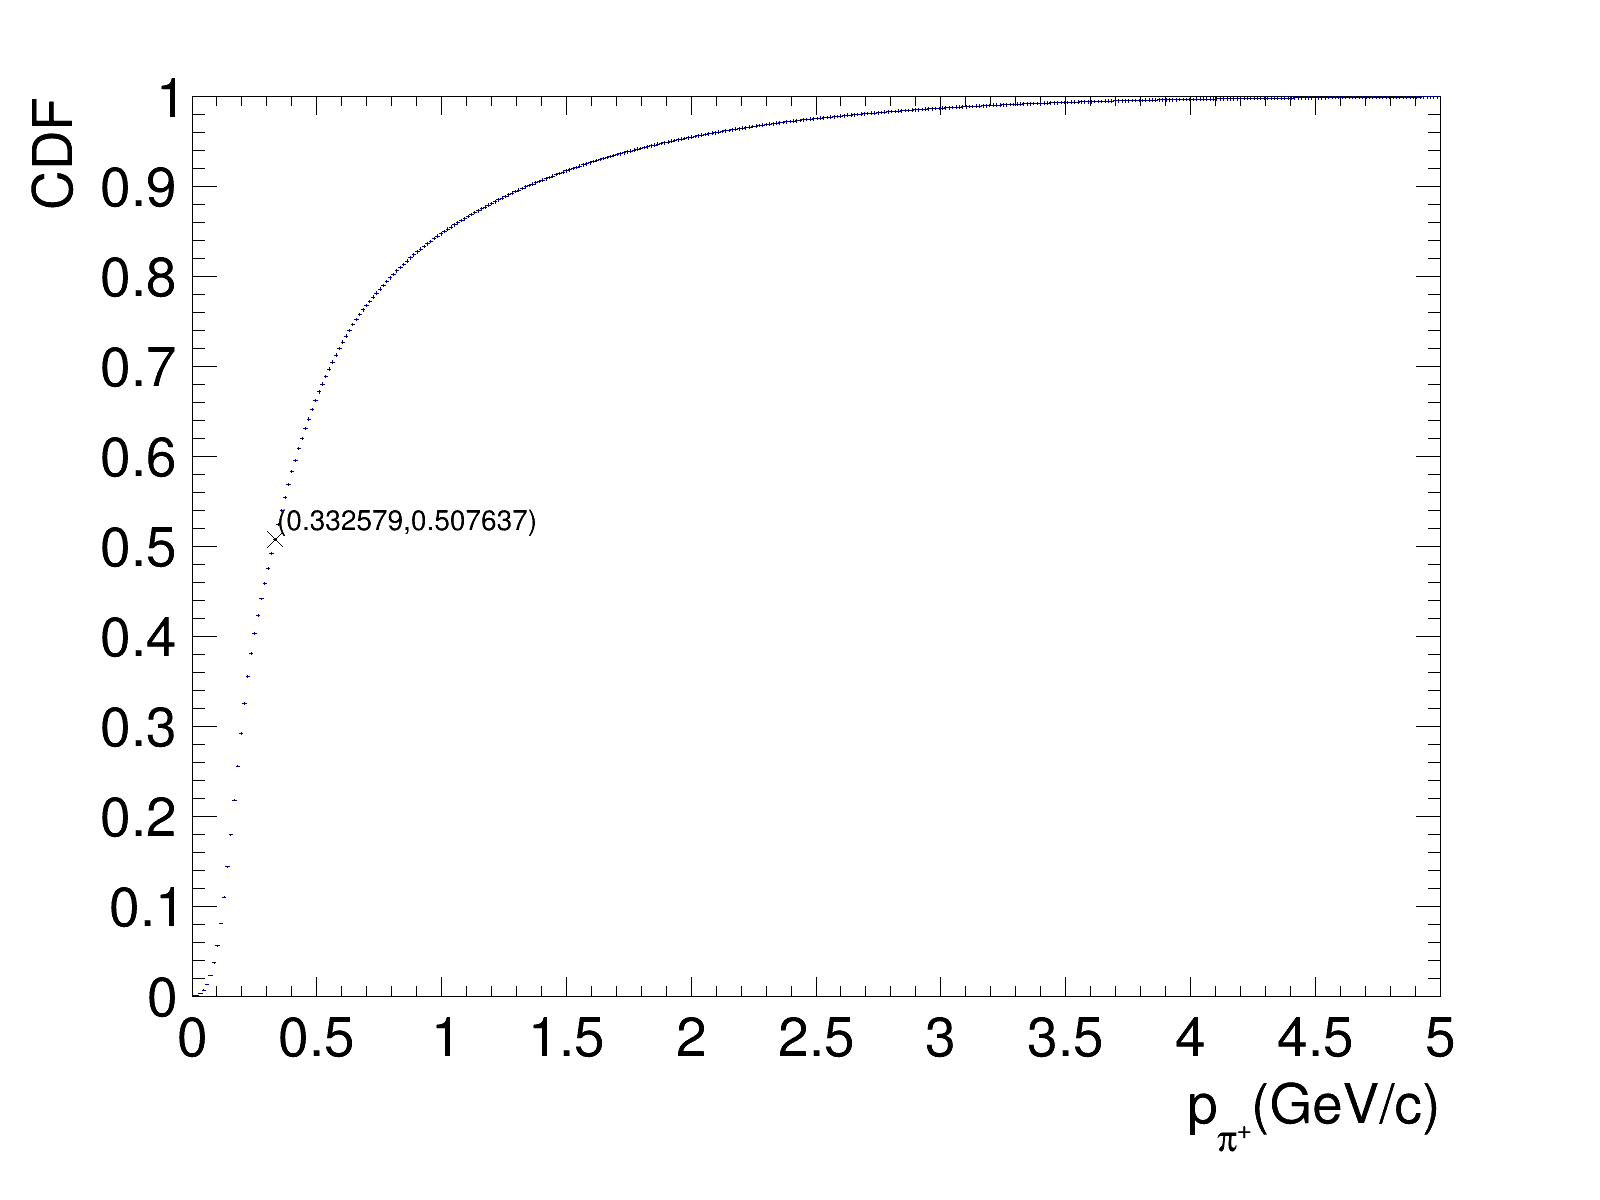
\includegraphics[width=\textwidth]{figures/sel/inclusive_pion_mom_CDF_0.5.png}
                    \caption{Primary pion momentum cumulative distribution. The median momentum is about $300~\mevc$.}
                    \label{subfig:pi-mom-cum}
               \end{subfigure}
               \begin{subfigure}{\dbfigwid\textwidth}
                    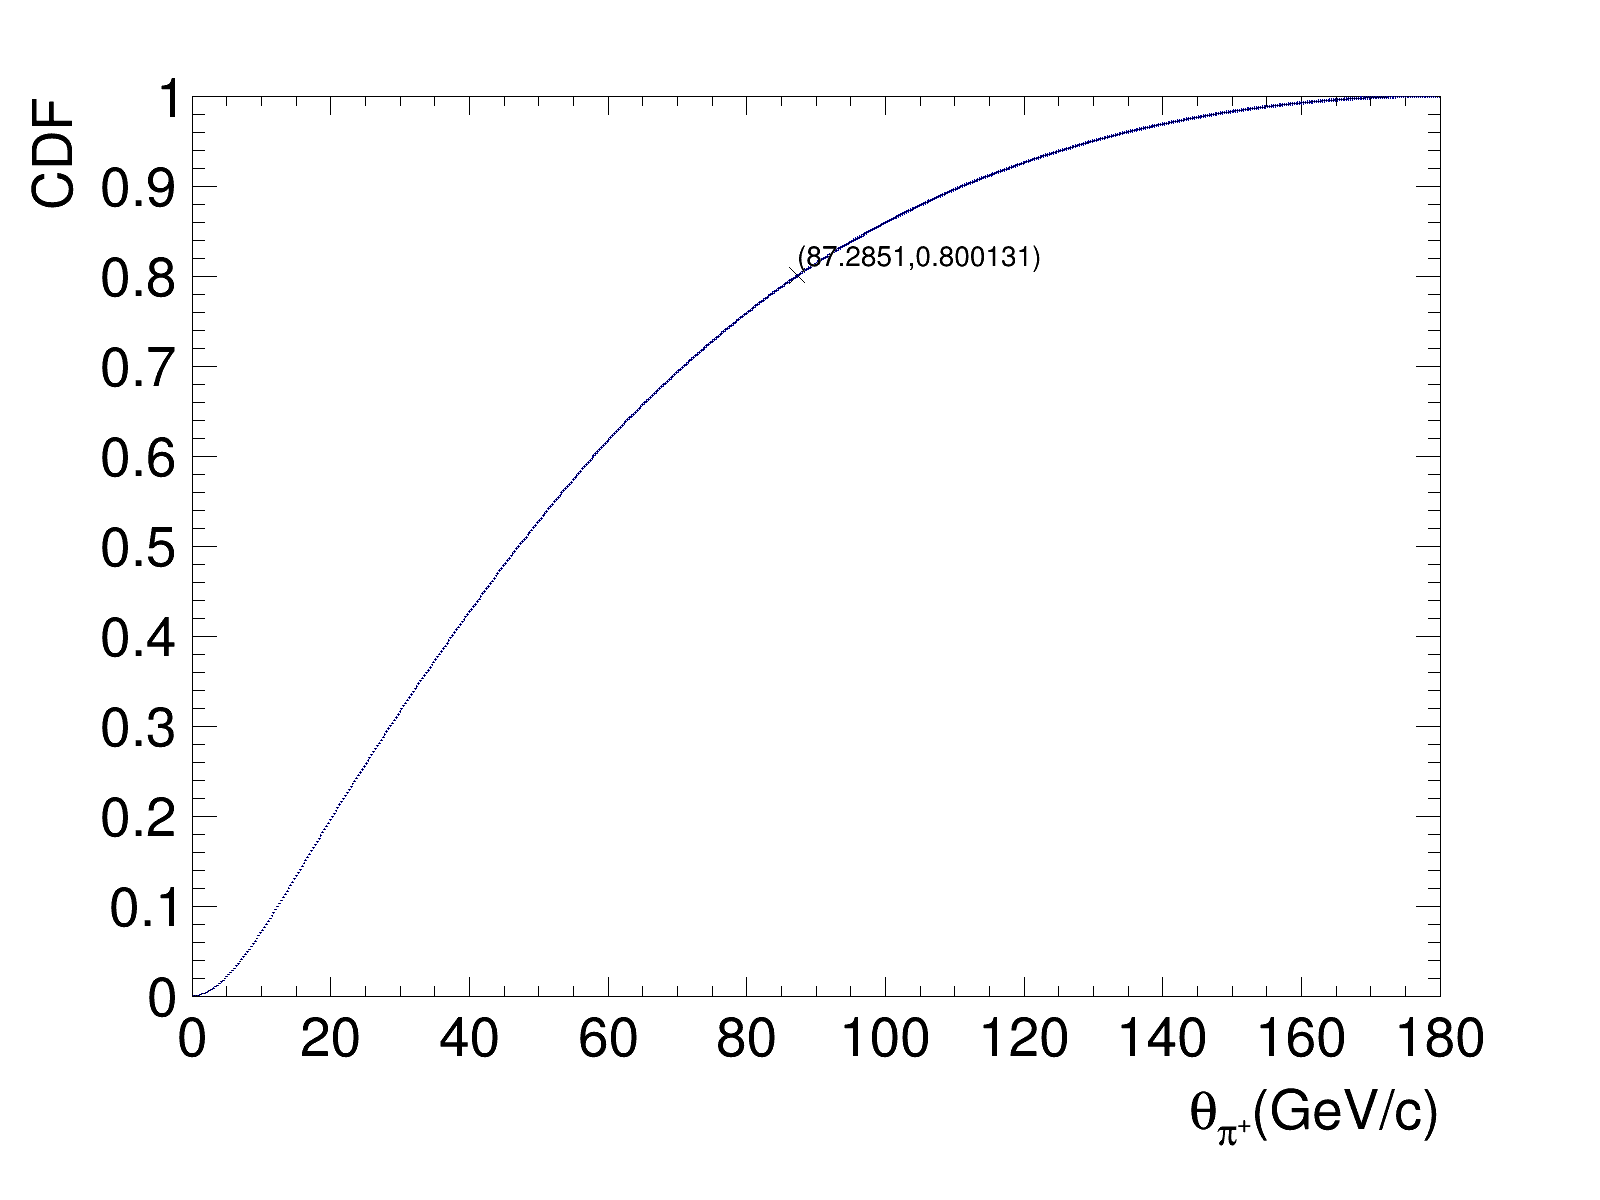
\includegraphics[width=\textwidth]{figures/sel/inclusive_pion_theta_CDF_0.8.png}
                    \caption{Primary pion angle cumulative distribution. The $80\%$ angle is $87^\circ$.}
                    \label{subfig:pi-theta-cum}
               \end{subfigure}
          \end{figure}
               
          The median momentum is approximately $300~\mevc$, with about $30\%$ of pions having momentum below $200~\mevc$ and $80\%$ below $800~\mevc$. 
          Similarly, the pion angle distribution, depicted in Fig.~\ref{subfig:pi-theta-cum}, shows that approximately $80\%$ of pions have an angle below $87^\circ$.

          The second step is to simulate pion propagation in SFGD with the relevant kinematics. 
          A total of six samples, each containing 10,000 events, were simulated with pions traveling at momenta of $200~\mevc$, $300~\mevc$, and $800~\mevc$, and angles of $0^\circ$ and $70^\circ$. 
          Since SFGD reconstruction is largely independent of pion direction, the $70^\circ$ samples serve as consistency checks. 
          For each sample, the fate of each pion was determined using the truth information.

          A total of ten fate topologies are defined as follows:
          \begin{enumerate}
          \item \textbf{DK@rest (Good)} – The pion decays at rest, and the total number of true trajectories is three, corresponding to $\pip$, $\mu$, and the ME exactly. 
          This represents a clean pion decay-at-rest event.
          \item \textbf{DK@rest (Dirty)} – Similar to the previous fate, but the total number of true trajectories exceeds three. 
          The additional trajectories are mostly electromagnetic showers due to the ME.
          \item \textbf{DK@flight} – The pion decays with non-zero momentum, resulting in a relatively large starting momentum for the daughter muon.
          \item \textbf{Elastic Knock-out} – The pion undergoes secondary interactions (SI), leading to the liberation of an additional proton. 
          The pion continues to propagate and decay, but its range is no longer well correlated with its starting momentum.
          \item \textbf{Deflection} – The pion undergoes SI. 
          No additional particles are produced, but its direction changes.
          \item \textbf{Absorption} – Another type of SI where the pion does not emerge from its interaction with the nucleus, so no ME is present.
          \item \textbf{Charge Exchange} – The $\pip$ is converted to a $\piz$ via a charge exchange interaction with the nucleus. 
          Since $\piz$ decays much faster, no ME is present.
          \item \textbf{$\pim$} – While there is no single interaction that can convert a $\pip$ to a $\pim$, this fate—where a $\pim$ appears as one of the daughters of the $\pip$—is observed, albeit rarely, due to complex pion SI within the nucleus.
          \item \textbf{Escaped} – The pion escapes SFGD before decaying. 
          Regardless of its subsequent decay, the potential ME cannot be detected in SFGD.
          \item \textbf{Others} – This category includes all uncategorized events, such as cases where the pion produces delta electrons or undergoes bremsstrahlung. 
          These events are relatively rare and do not require special treatment.
          \end{enumerate}

          Fates 1 through 3 involve pions that decay before any secondary interactions, i.e., pions decay via the chain $\pi \rightarrow \mu \rightarrow e$. 
          Thus, these pions can be tagged by the presence of the ME. 
          However, as illustrated in Sec.~\ref{sec:tl-wp}, the trackless technique relies on the extremely short distance traveled by the daughter muon. 
          Pions decaying in flight result in a longer distance traveled by the daughter muon, making them unsuitable for the trackless technique.

          Fates 4 through 8 involve pions that undergo secondary interactions, resulting in the absence of the ME, except for those that experience deflection, which also renders them unsuitable for the trackless technique. 
          The range of a deflected pion does not correlate well with its momentum, further disqualifying it from being reconstructed by the trackless technique. 
          In summary, the trackless technique is most applicable to Fates 1 and 2.

          The fate distributions are shown in Fig.~\ref{fig:pi-fate}. 
          For the $200~\mevc$ samples, both at $0^\circ$ and $70^\circ$, more than $70\%$ of the pions fall into Fates 1 and 2. 
          In the $300~\mevc$ samples, this fraction drops to $30\%$ for the $0^\circ$ angle and about $12\%$ for the $70^\circ$ angle. 
          This trend is expected because as pion momentum increases, the decay length increases, and the probability of secondary interactions rises. 
          The further decrease observed at $70^\circ$ is attributed to an increased escape fraction. 
          The geometry of SFGD, being much shorter in the vertical direction, facilitates the escape of high-angle pions. 
          For $800~\mevc$ pions, the decay length is too long for SFGD, resulting in a significant increase in the escape fraction—approximately $30\%$ at $0^\circ$ and $50\%$ at $70^\circ$. 
          The unescaped pions are those that have undergone secondary interactions, rendering them unreconstructable by the trackless technique at this high momentum.

          \begin{figure}[t]
               \centering
               \begin{subfigure}{\dbfigwid\textwidth}
                    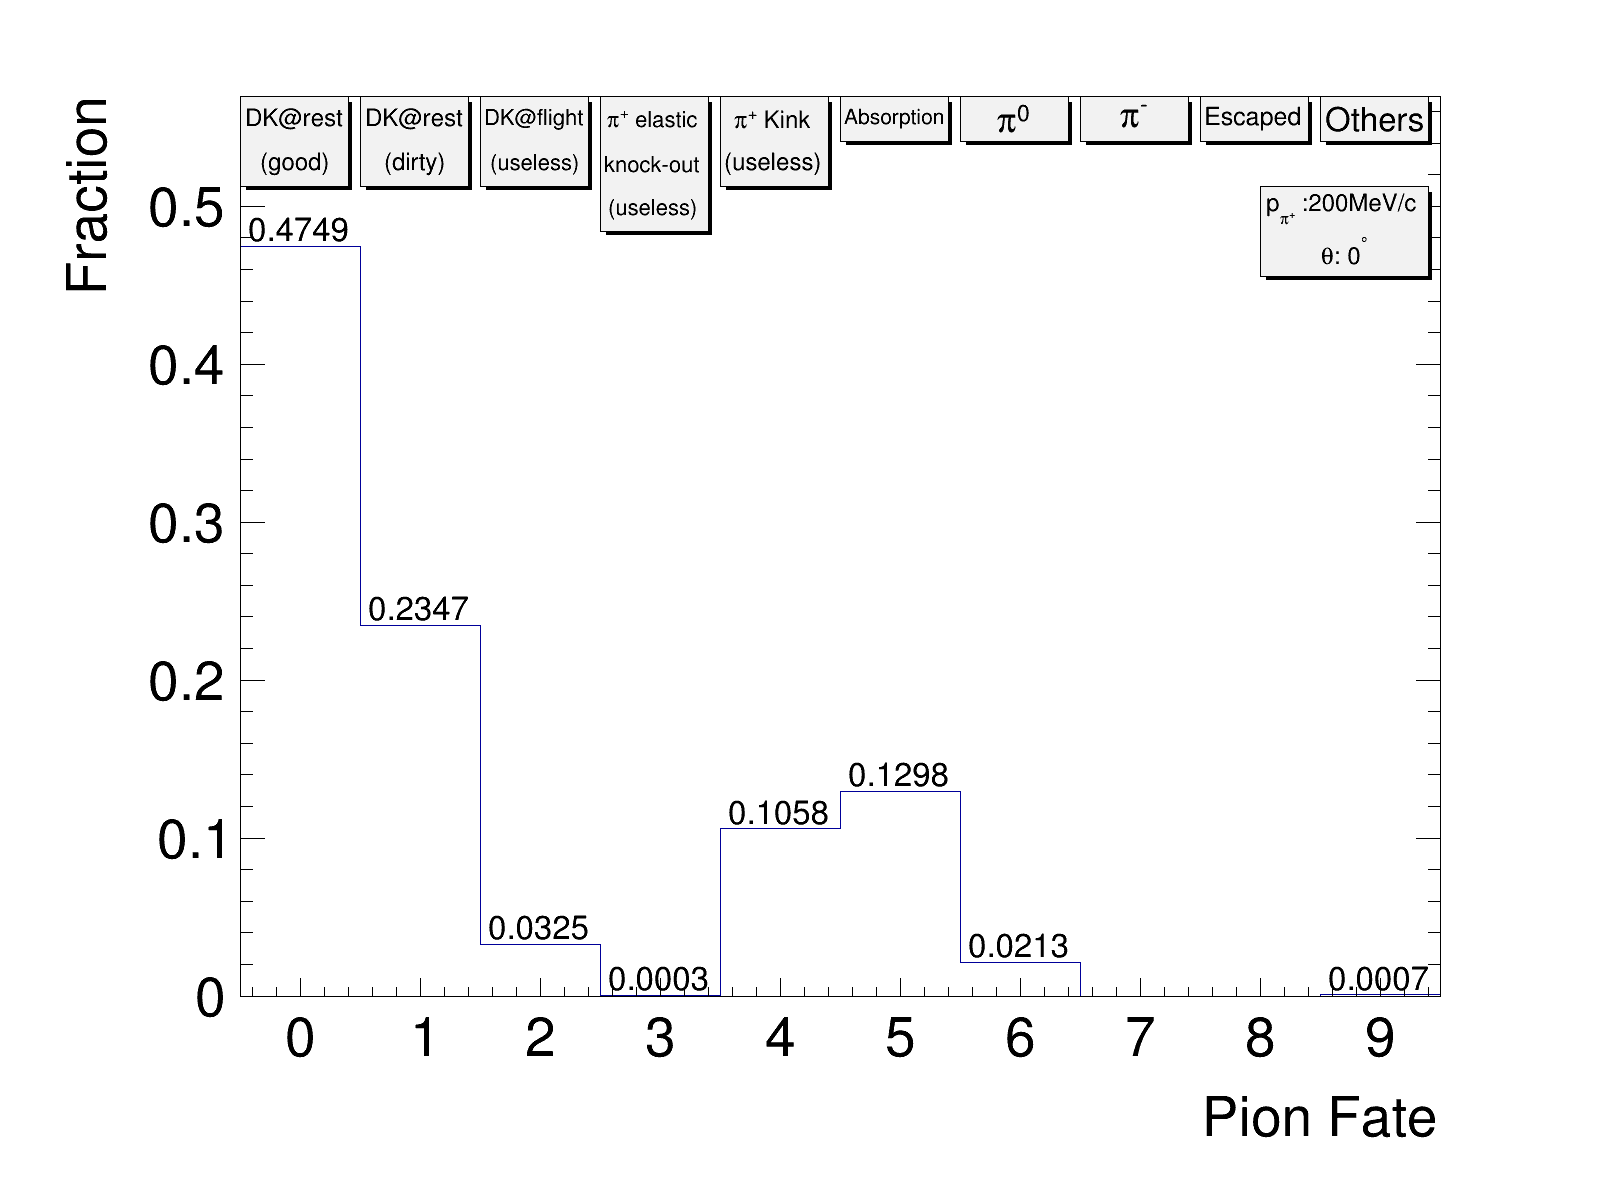
\includegraphics[width=\textwidth]{figures/sel/pion_fate_200_0.png}
                    \caption{$\ppi=200\mevc$ and $\tpi=0^\circ$.}
                    \label{subfig:pi-fate-200-0}
               \end{subfigure}
               \begin{subfigure}{\dbfigwid\textwidth}
                    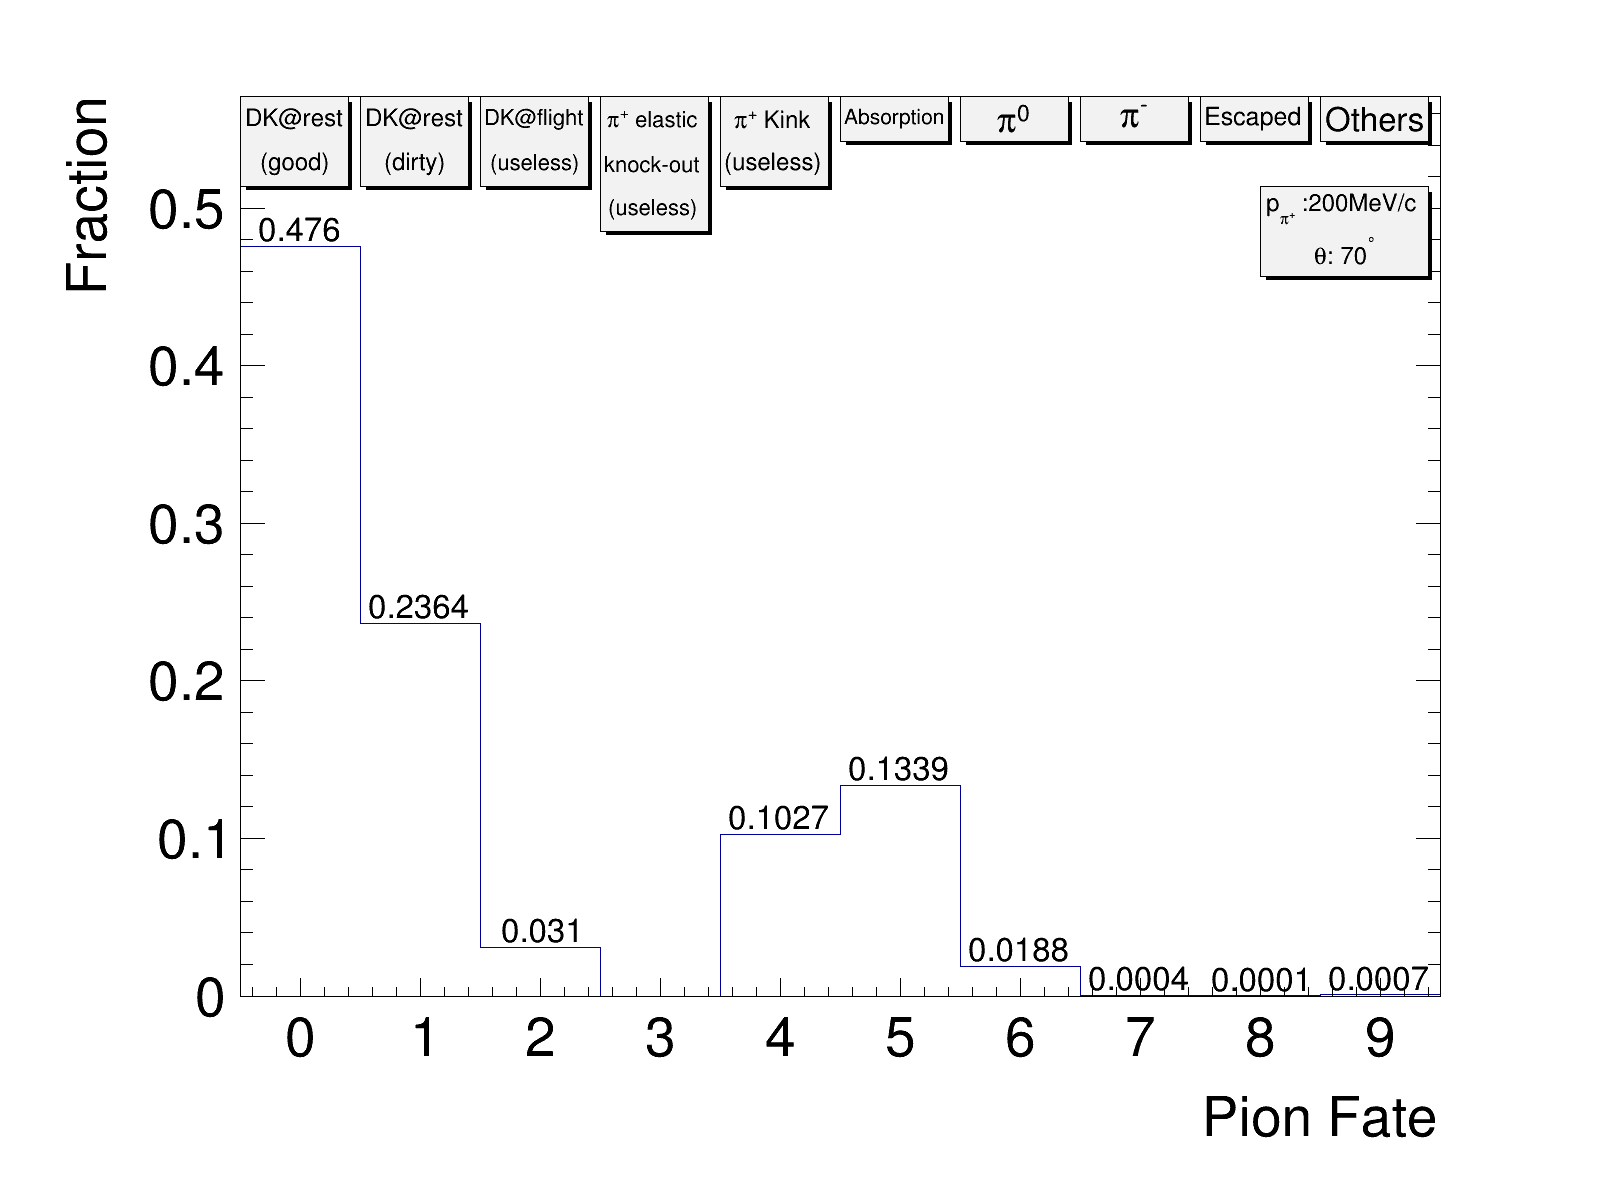
\includegraphics[width=\textwidth]{figures/sel/pion_fate_200_70.png}
                    \caption{$\ppi=200\mevc$ and $\tpi=70^\circ$.}
                    \label{subfig:pi-fate-200-70}
               \end{subfigure}
              \\
               \begin{subfigure}{\dbfigwid\textwidth}
                    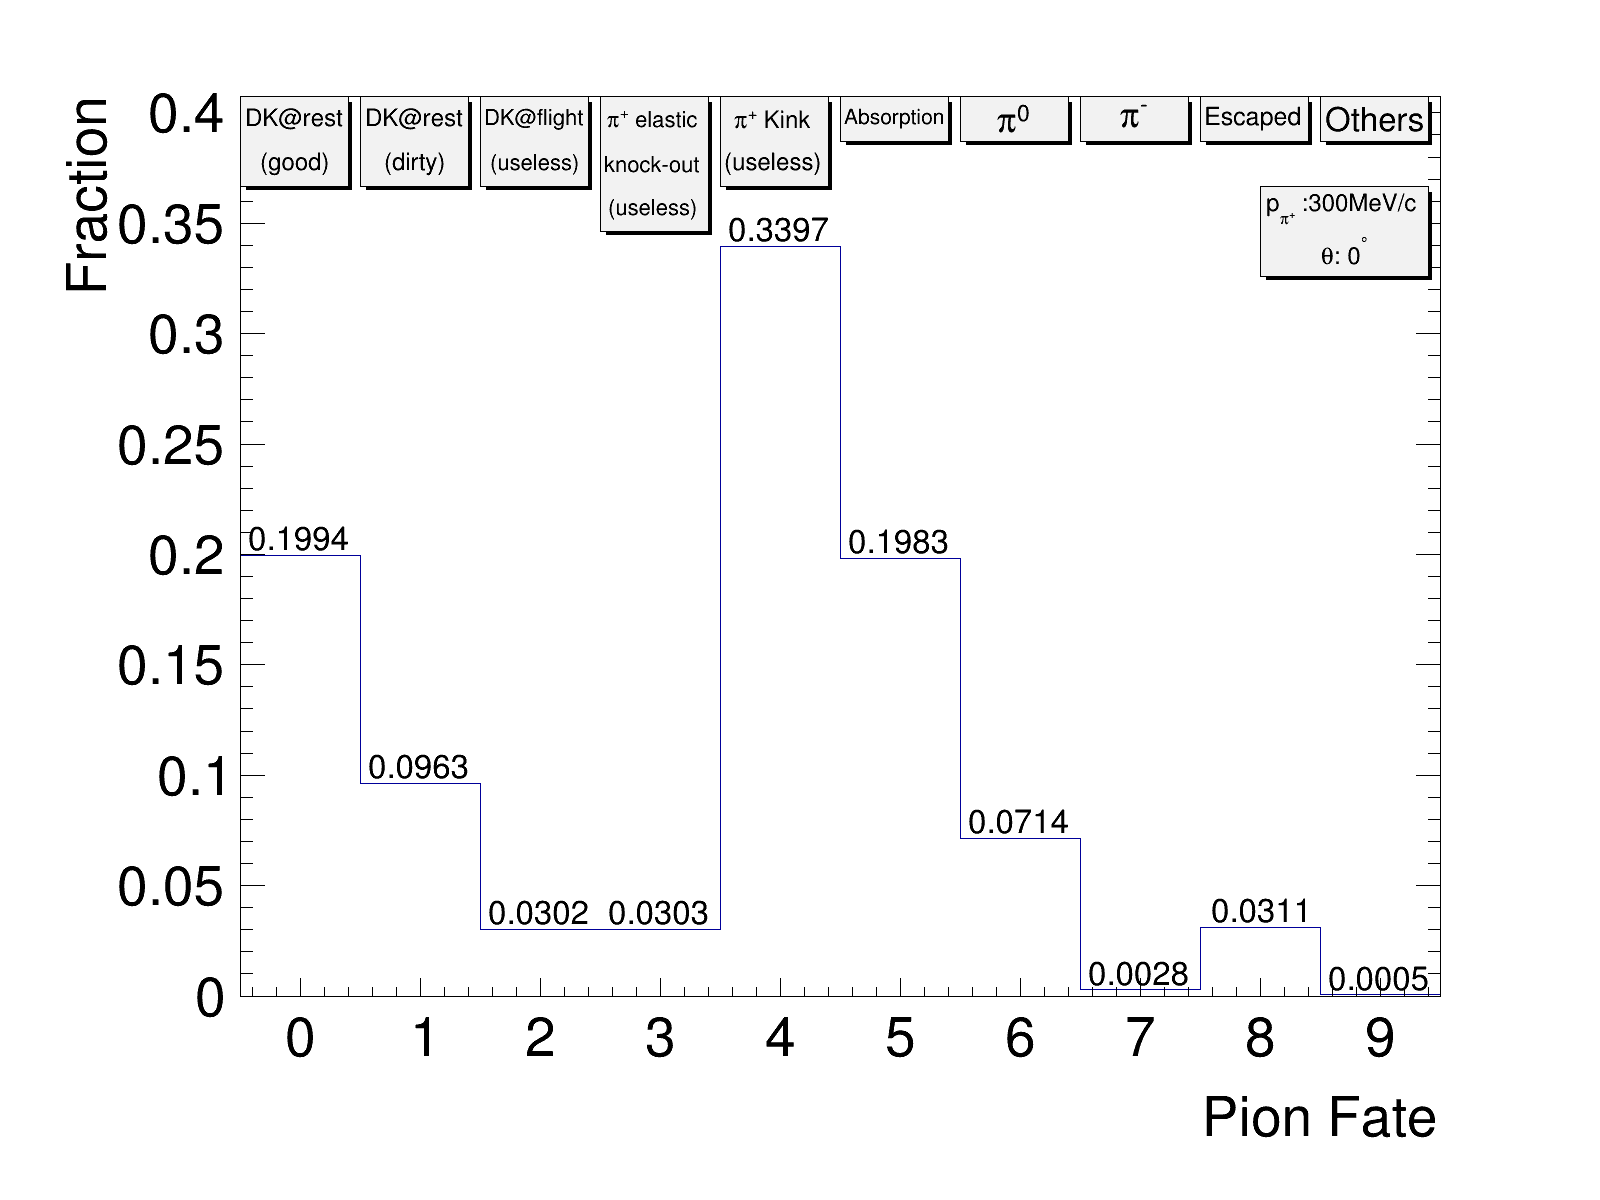
\includegraphics[width=\textwidth]{figures/sel/pion_fate_300_0.png}
                    \caption{$\ppi=300\mevc$ and $\tpi=0^\circ$.}
                    \label{subfig:pi-fate-300-0}
               \end{subfigure}
               \begin{subfigure}{\dbfigwid\textwidth}
                    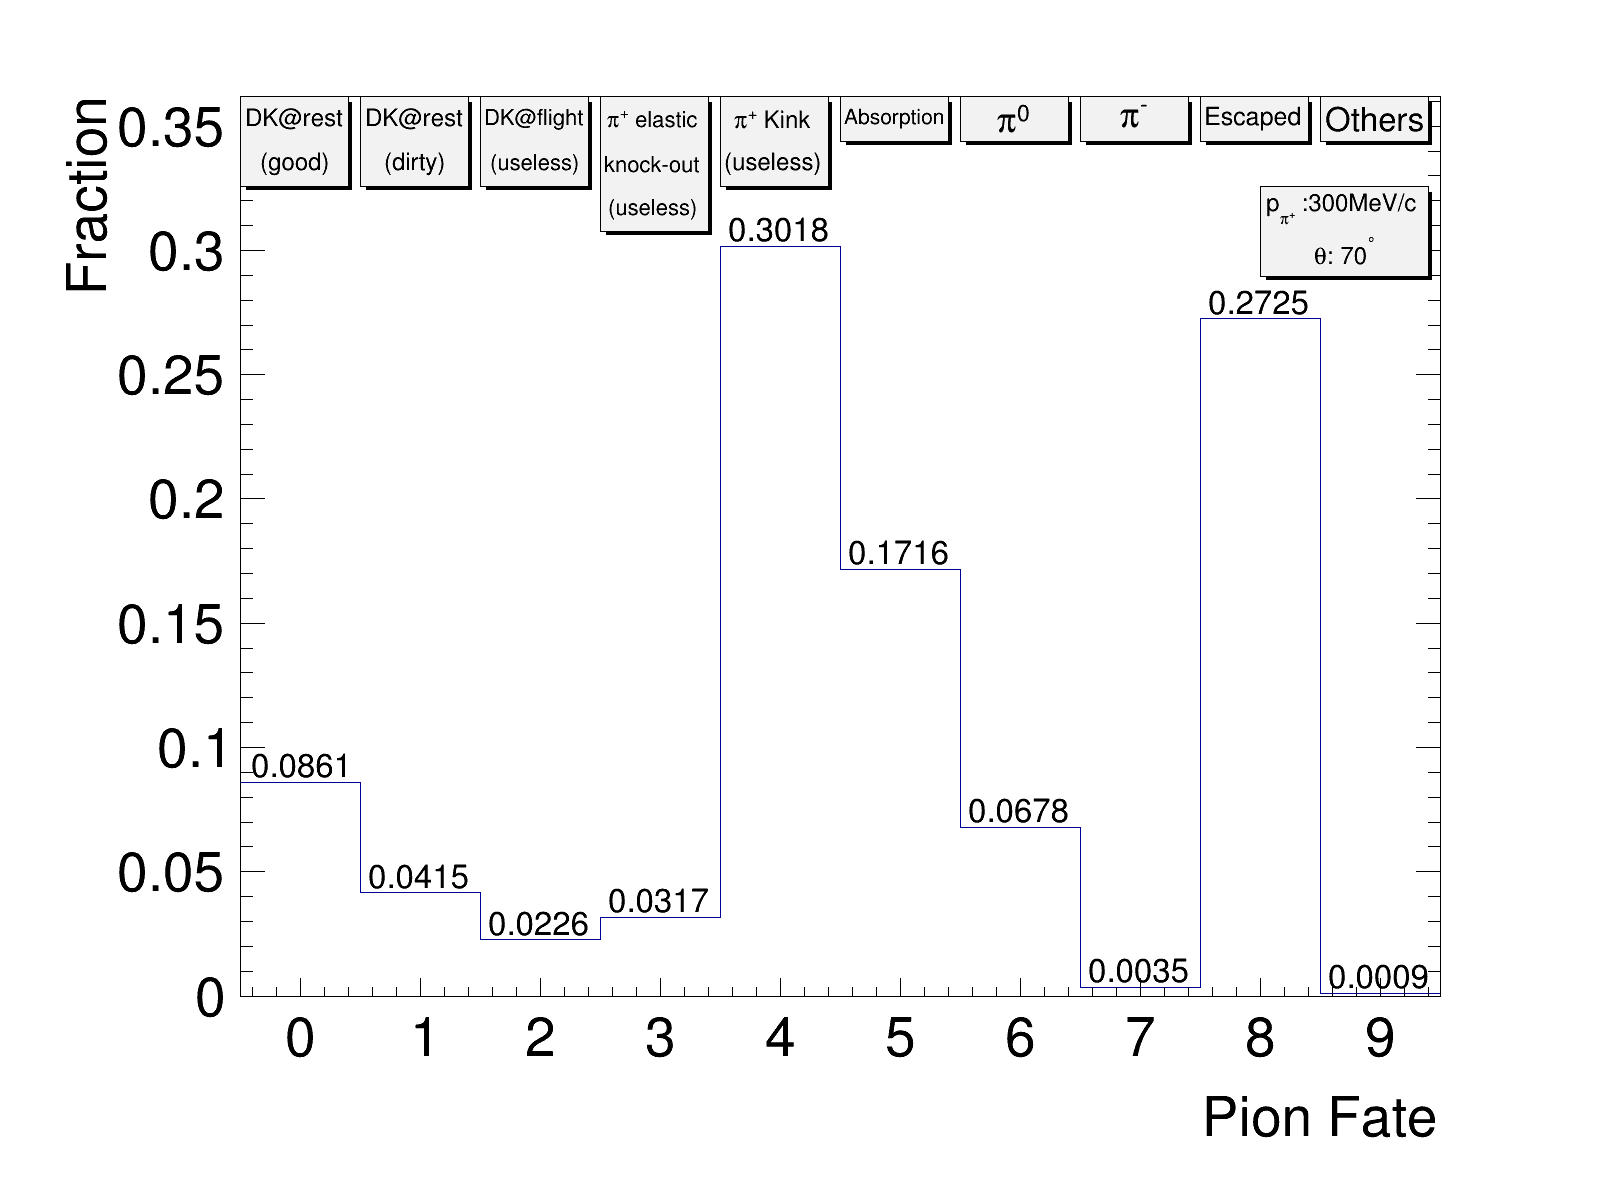
\includegraphics[width=\textwidth]{figures/sel/pion_fate_300_70.png}
                    \caption{$\ppi=300\mevc$ and $\tpi=70^\circ$.}
                    \label{subfig:pi-fate-300-70}
               \end{subfigure}
              \\
               \begin{subfigure}{\dbfigwid\textwidth}
                    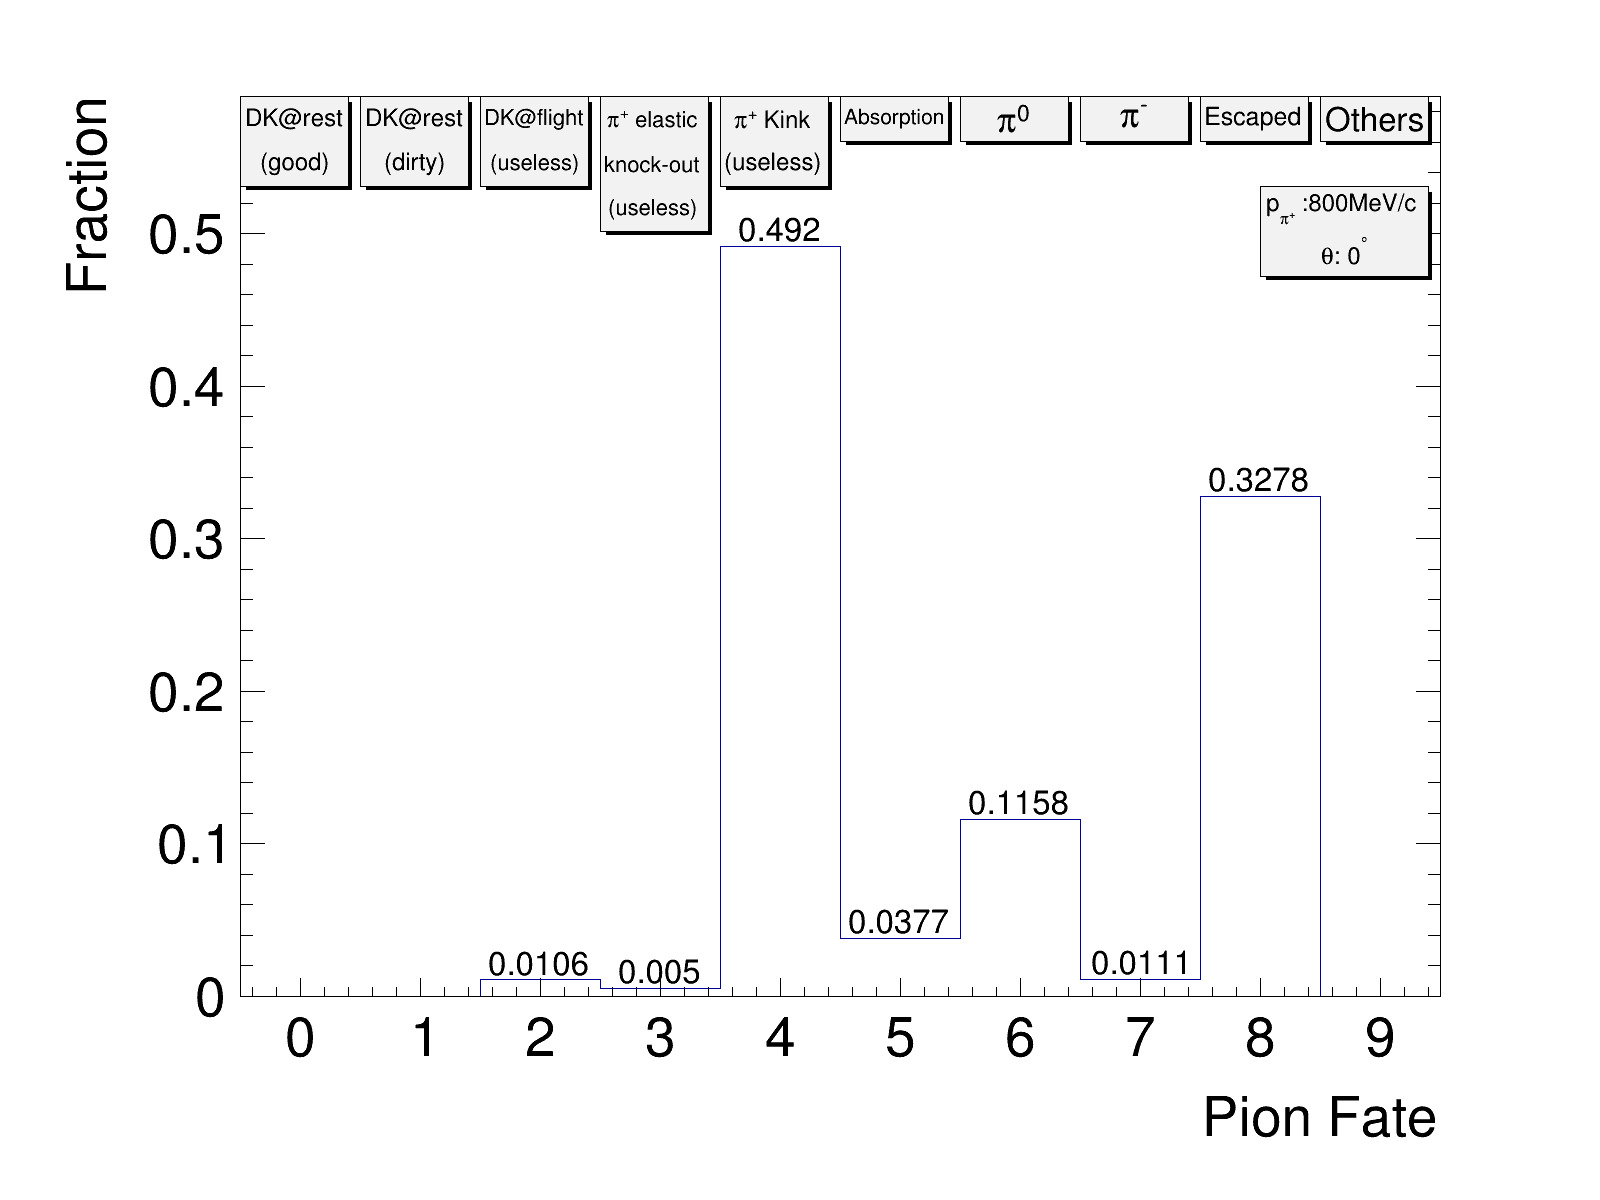
\includegraphics[width=\textwidth]{figures/sel/pion_fate_800_0.png}
                    \caption{$\ppi=800\mevc$ and $\tpi=0^\circ$.}
                    \label{subfig:pi-fate-800-0}
               \end{subfigure}
               \begin{subfigure}{\dbfigwid\textwidth}
                    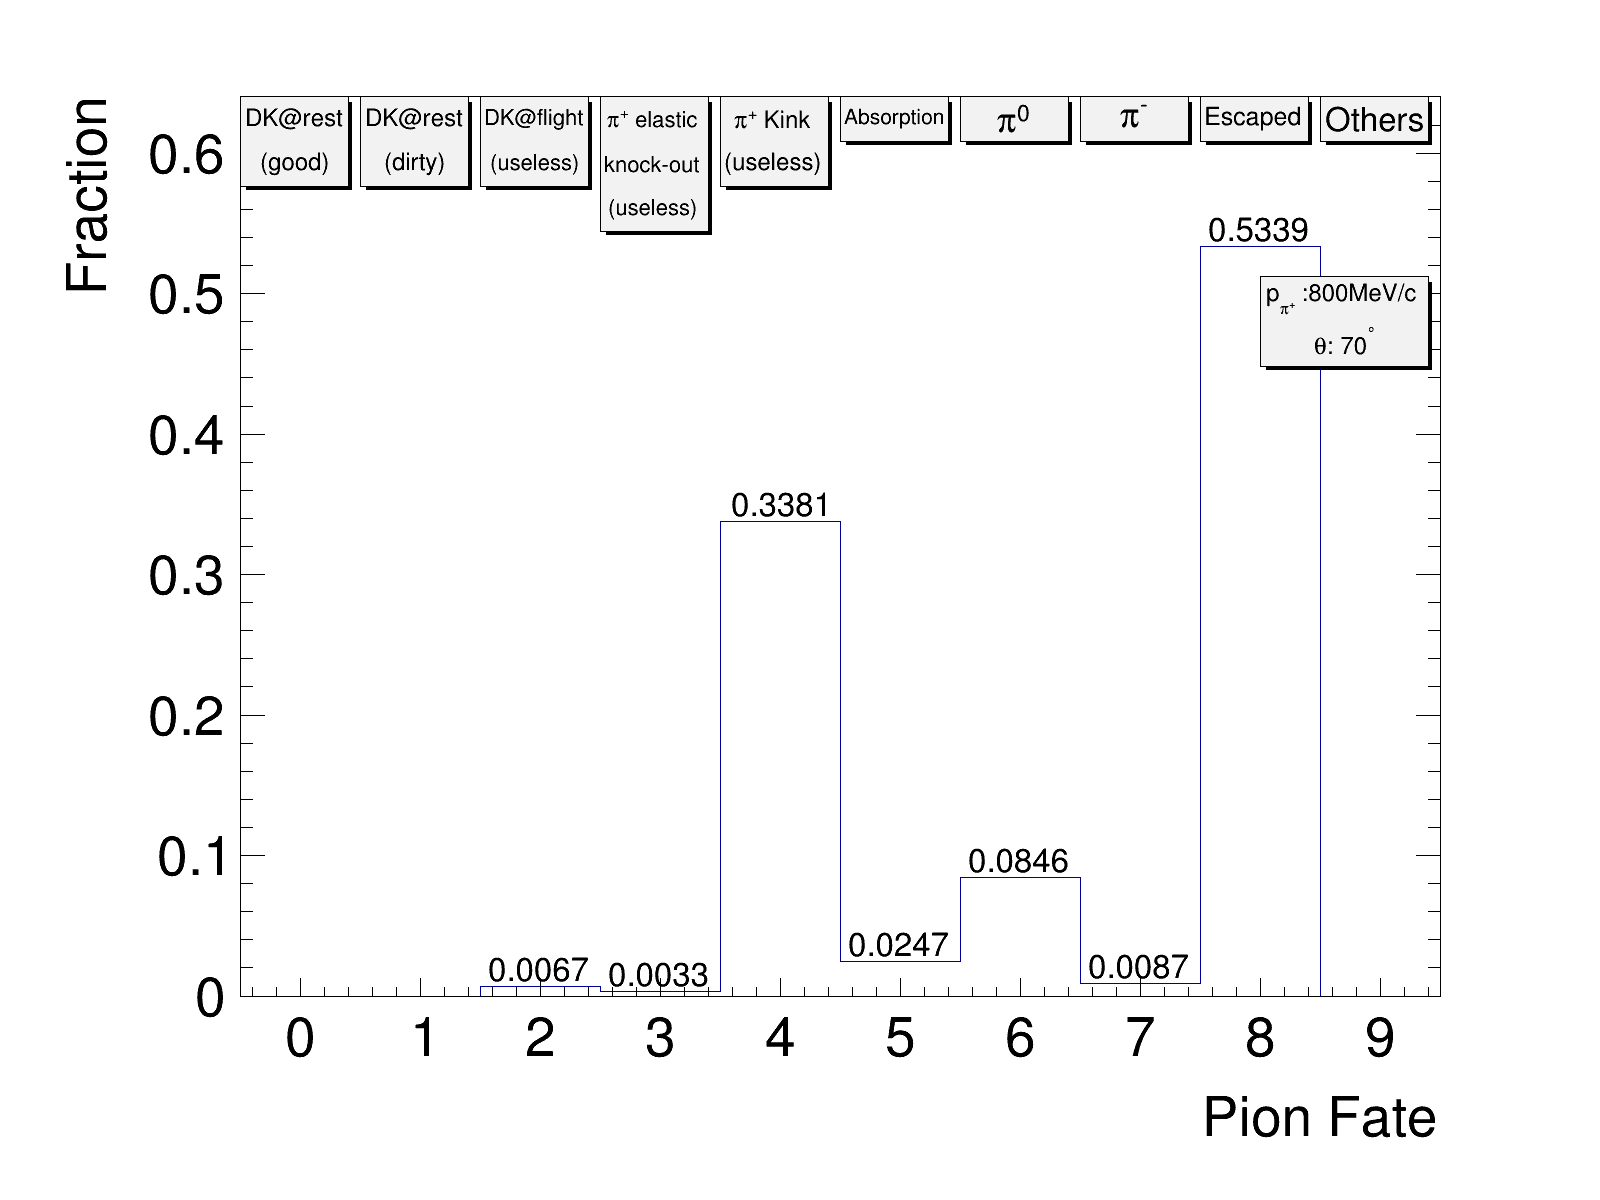
\includegraphics[width=\textwidth]{figures/sel/pion_fate_800_70.png}
                    \caption{$\ppi=800\mevc$ and $\tpi=70^\circ$.}
                    \label{subfig:pi-fate-800-70}
               \end{subfigure}
               \caption{Pion fates in the SFGD for different combinations of pion kinematics}
               \label{fig:pi-fate}
            \end{figure}
       
          This preliminary study demonstrates that a considerable fraction of the primary pions produced in SFGD have relatively low momentum ($<200~\mevc$). 
          For these pions, the majority decay at rest, producing an ME that can be utilized in the trackless technique. 
          Thus, the trackless technique is applicable to approximately $30\%$ of the total pion events in SFGD, making it a significant reconstruction method to develop.

     \subsection{Working Principles}
     \label{sec:tl-wp}
          The trackless technique is an advancement of previous methods. 
          It was first attempted in MINER$\nu$A~\cite{poster:minerva-pime} and in the Fine Grain Detectors of ND280~\cite{poster:minerva-pime}. 
          In MINER$\nu$A, a reconstructed cluster must be identified as a pion candidate. 
          In contrast, ND280 includes a prototype of the trackless reconstruction; however, it is integrated with other pion reconstruction methods, and its full potential has not yet been explored.

          This reconstruction technique is based on two key aspects of the pion decay chain, $\pi \rightarrow \mu \rightarrow e$:

          \begin{enumerate}
          \item \textbf{Delayed Michel Electron (ME) Signal:} The ME, as the grandchild in the decay chain, produces a delayed signal that occurs on a much longer timescale compared to other processes, such as $\piz$ decay. 
          Consequently, the presence of the primary pion can be inferred from the delayed ME signal in the SFGD.
          
          \item \textbf{Kinematic Determination via Energy-Momentum Conservation:} The pion decay, $\pi \rightarrow \mu + \nu$, is a two-body process. 
          The kinematics of the daughter particles are entirely determined by energy-momentum conservation. 
          When a pion decays at rest, the daughter muon moves only about $0.12~\textrm{cm}$. 
          Therefore, the starting point of the ME provides a reliable estimate of the pion's endpoint.
          \end{enumerate}

          Using the distance between the primary neutrino interaction vertex and the ME starting point, the pion momentum can be reconstructed by range. 
          An empirical relationship between the pion's kinetic energy and its range was established using a PGUN sample, as shown in Fig.~\ref{fig:pi-mombr-fit}. 
          The PGUN sample initiates pions from the center of SFGD and propagates them isotropically. 
          It comprises $500,000$ events with kinetic energies uniformly distributed between $20~\mev$ and $200~\mev$. 
          The $\log_{10}$ of the true kinetic energy is plotted against the true pion length in Fig.~\ref{fig:pi-mombr-fit}. 
          A fourth-order polynomial fits the central region of the plots well, accurately capturing the relationship between kinetic energy and range.

          \begin{figure}[h]
          \centering
          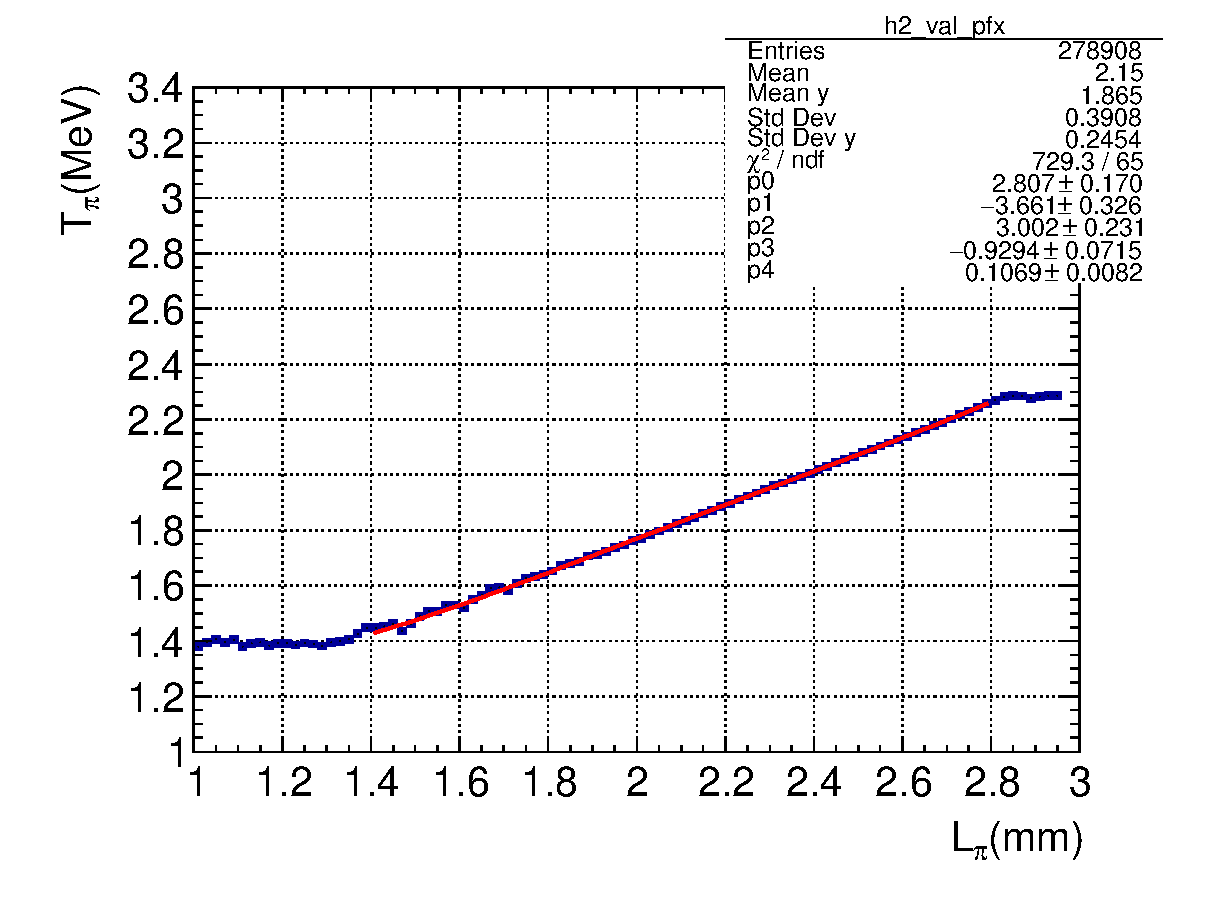
\includegraphics[width=\sgfidwid\textwidth]{figures/sel/pi_len_pi_len_vs_pi_ke_hist2d_al0_true_nokink.eps} 
          \caption{A degree 4 polynomial fit of $\log_{10}{T_\pi}$ against $\log_{10}{L_\pi}$, where $T_\pi$ and $L_\pi$ are the kinetic energy and the range of the pion, respectively. The $p_i$'s are the corresponding coefficients of the term of order $i$. The fit is satisfactory, with a $\chi^2/\textrm{n.d.f.}$ value close to 1.}
          \label{fig:pi-mombr-fit}
          \end{figure}

     \subsection{Implementation}
     \label{sec:tl-imp}
          The pion trackless reconstruction is integrated into my $\numuccopi$ selection, which builds upon the existing $\numucc$-inclusive selection. 
          Therefore, it is appropriate to discuss the trackless technique within the context of the $\numuccopi$ selection.

          The $\numucc$-inclusive selection identifies the primary vertex position and the primary muon, providing the trackless reconstruction with a reliable approximation of the pion's starting point. 
          The following steps are implemented to identify suitable ME candidates and reconstruct the pion momentum in the $\numuccopi$ selection:
          \begin{itemize}
          \item \textbf{Step 0 - $\numucc$-inclusive Selection}
          \item \textbf{Step 1 - Find Suitable ME Candidates}
          \item \textbf{Step 2 - One Trackless Pion Cut}
          \item \textbf{Step 3 - Kink Cut}
          \item \textbf{Step 4 - Background Reduction}
          \end{itemize}
          \textbf{Find Suitable ME Candidates} – Iterate through all delayed reconstructed objects with more than one hit. 
          If an object occurs $30.0~\textrm{ns}$ after the primary vertex time, it is saved as a potential ME candidate. 
          However, ME candidates may trigger showers, resulting in additional delayed reconstructed objects. 
          To distinguish the true ME from these secondary objects, the "prompt energy" technique used by MINERvA~\cite{Zhang:2016glf} is employed. 
          Prompt energy refers to the energy deposited by the short muon and pion. 
          Although these particles may have insufficient energy to form a reconstructable track, they still deposit energy much earlier than the ME onset. 
          Therefore, by examining the energy deposition within $30~\textrm{mm}$ around both ends of an ME candidate, it can be determined if energy was deposited $30~\textrm{ns}$ prior, confirming the suitability of the ME candidate. 
          Additionally, if the primary muon is contained within SFGD, it may also decay and produce an indistinguishable ME based solely on time delay. 
          To address this, an additional check excludes ME candidates near the end of the identified primary muon.

          \textbf{One Trackless Pion Cut} – Select events that have exactly one proper ME candidate.

          \textbf{Kink Cut} – Since the trackless reconstruction does not require the ME to be adjacent to a primary track, it cannot differentiate pions traveling directly from the primary interaction to decay at rest from those that have been deflected before decaying at rest. 
          To ensure accurate momentum-by-range reconstruction, events with deflected pions are rejected. 
          Specifically, any event with an ME connected to non-primary tracks is excluded.

          \textbf{Background Reduction} – Multiple background reduction steps are implemented, including an existing $\pi^0$ rejection developed by colleagues at T2K. 
          However, these measures are insufficient, as evidenced by the significant portion of CC-other backgrounds in Figs.~\ref{subfig:tlpi-ppi-bf-trknumcut-tpc}, \ref{subfig:tlpi-tpi-bf-trknumcut-tpc}, \ref{subfig:tlpi-ppi-bf-trknumcut-sfg}, and \ref{subfig:tlpi-tpi-bf-trknumcut-sfg}. 
          Therefore, based on a logical understanding of different event topologies, I developed a series of track number cuts and introduced a new concept called the "track family tree."

          An event topology resembles a family tree sideways. 
          The first generation consists of the primary tracks, while the second generation includes tracks connected to the ends of the primary tracks. 
          The family tree tracing step involves looping through all reconstructed tracks to build the family tree starting from the primary vertex. 
          One useful variable is the number of generations. 
          A $\numuccopi$ event should not have a large number of generations, as the primary pion can have an ME attached to its end without producing showers or multiple scatterings. 
          Therefore, the number of generations is required to be fewer than three. 
          Another associated variable is the number of lone tracks, which are not connected to any tracks in the family tree. 
          A clean $\numuccopi$ event should have a limited number of lone tracks, which could result from noise or low-energy scattering of the ME, leading to clusters isolated from the ME track. 
          Further details on the other track number cuts are provided in Appendix.~\ref{sec:app-tlpi-trknumcut}. 
          The overall impact of the track number cuts is illustrated by the topological decomposition of the pion kinematic distributions in Fig.~\ref{fig:tl-trknum-cut-res}.

            \begin{figure}
               \centering
               \begin{subfigure}{\dbfigwid\textwidth}
                    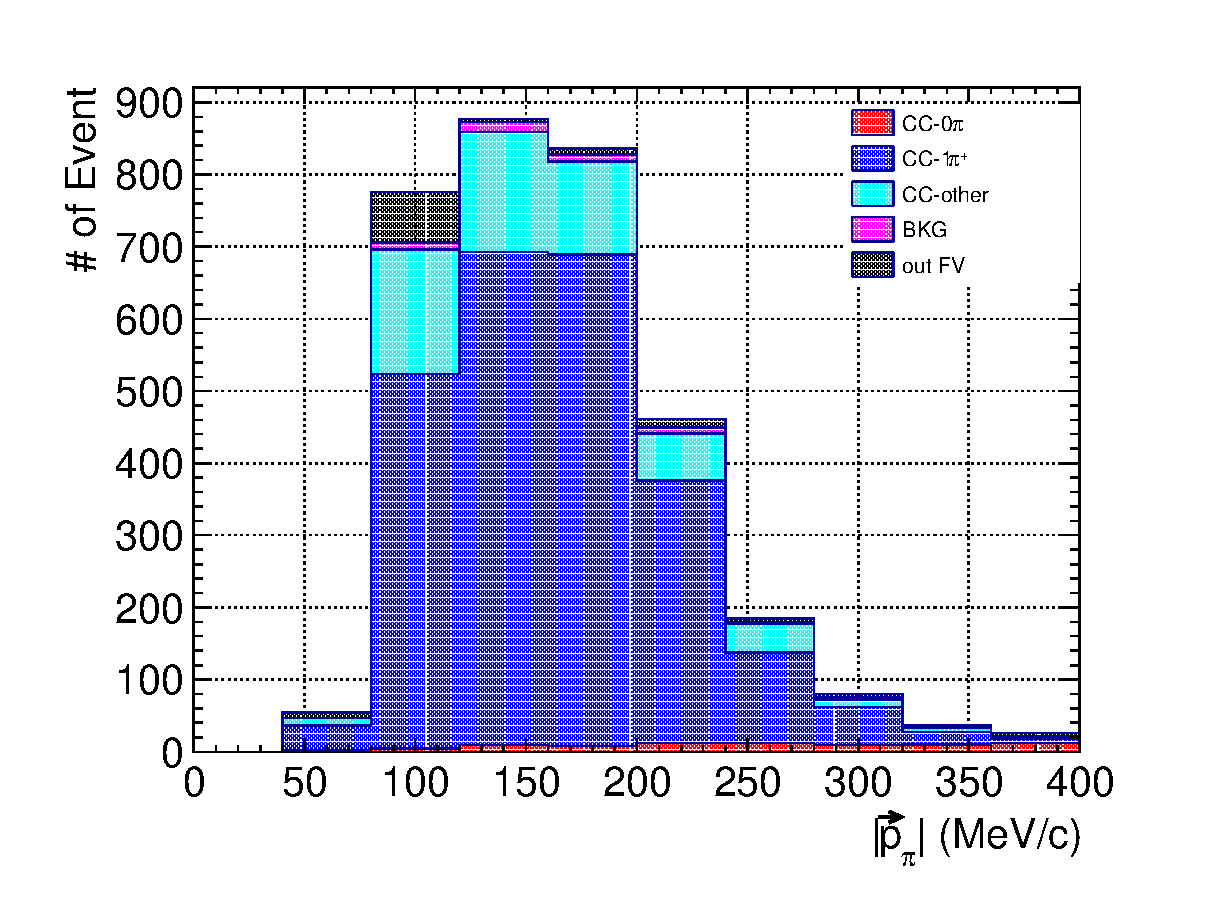
\includegraphics[width=\textwidth]{figures/sel/TPCmu_p_pi_stack_al8.eps}
                    \caption{TPC-$\mu$: $\ppi$ before track number cut.}
                    \label{subfig:tlpi-ppi-bf-trknumcut-tpc}
               \end{subfigure}
               \begin{subfigure}{\dbfigwid\textwidth}
                    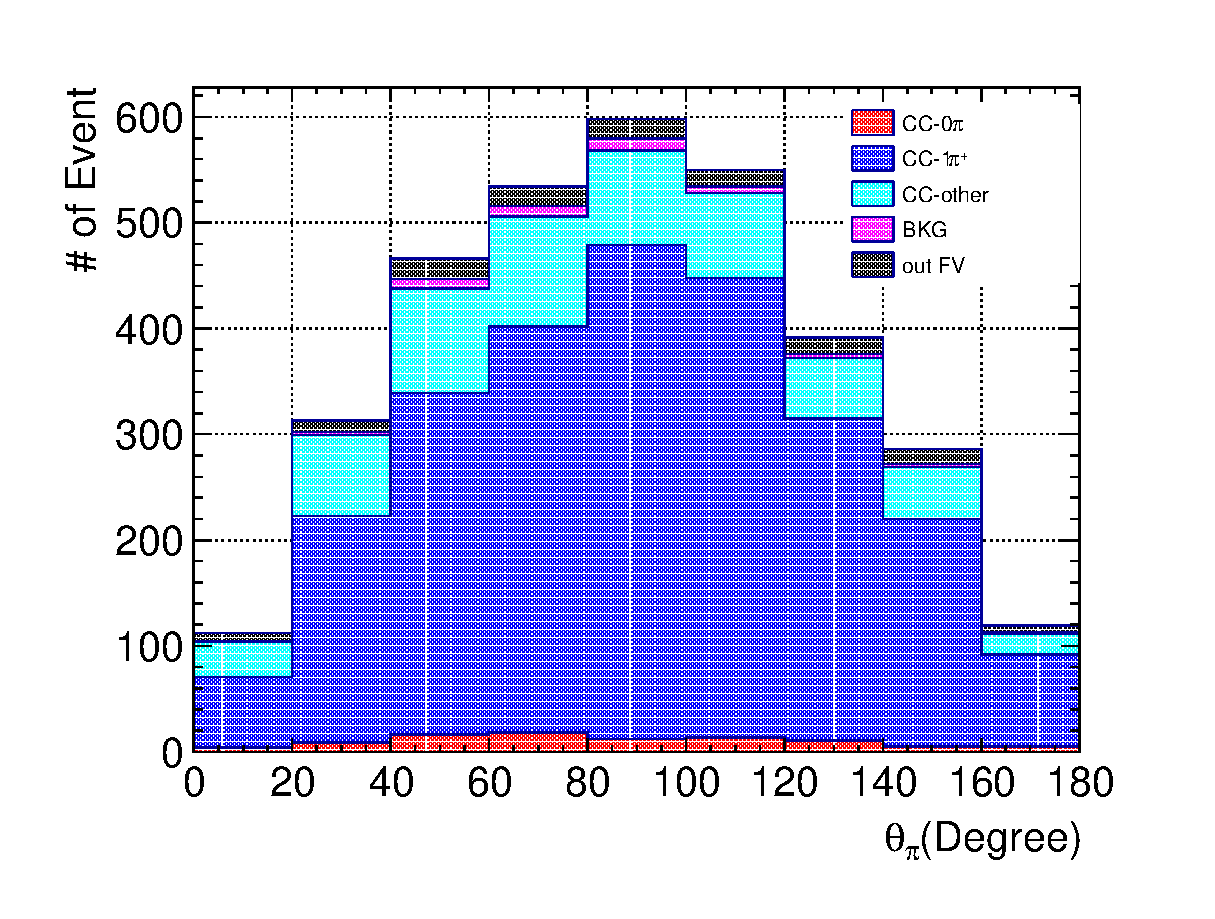
\includegraphics[width=\textwidth]{figures/sel/TPCmu_theta_pi_stack_al8.eps}
                    \caption{TPC-$\mu$: $\tpi$ before track number cut.}
                    \label{subfig:tlpi-tpi-bf-trknumcut-tpc}
               \end{subfigure}
               \\
               \begin{subfigure}{\dbfigwid\textwidth}
                    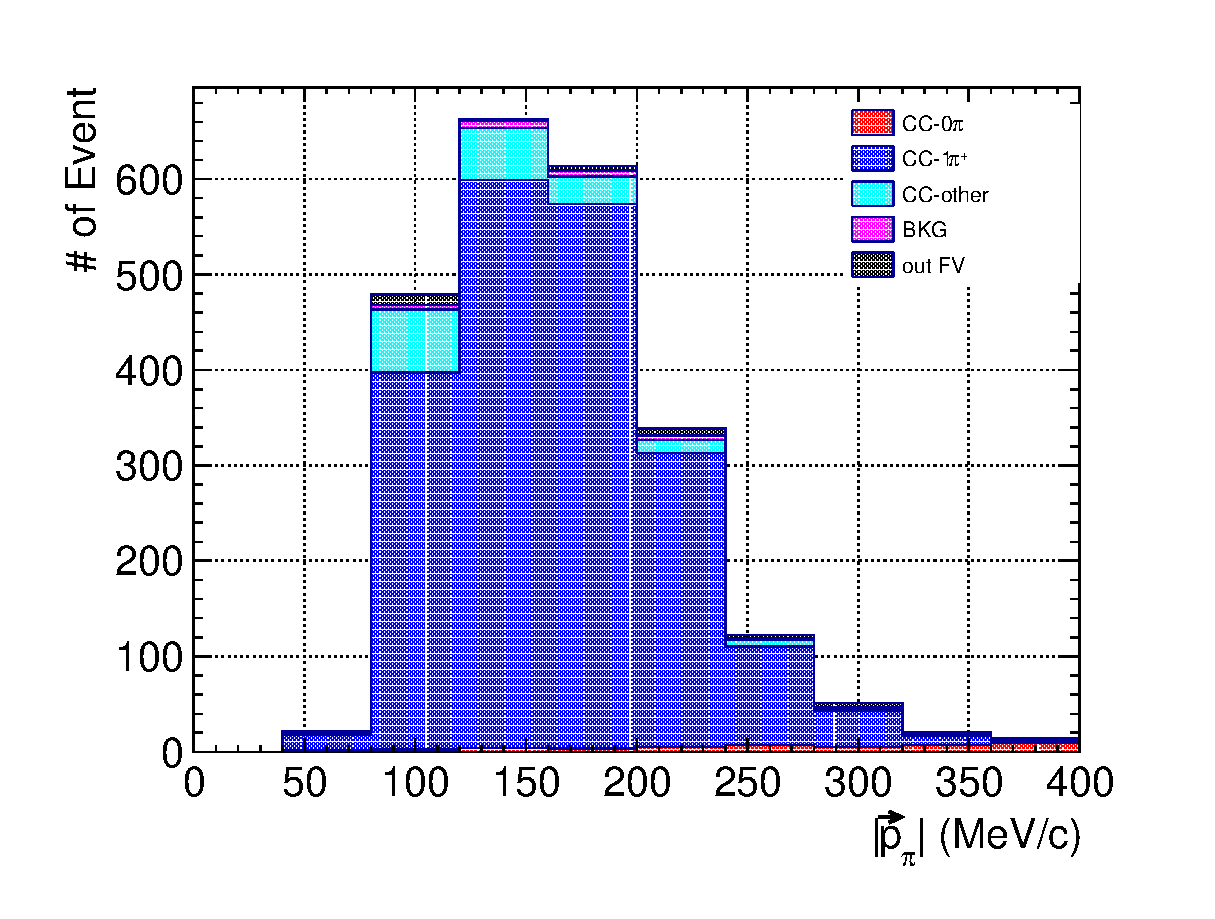
\includegraphics[width=\textwidth]{figures/sel/TPCmu_p_pi_stack_al9.eps}
                    \caption{TPC-$\mu$: $\ppi$ after track number cut.}
                    \label{subfig:tlpi-ppi-af-trknumcut-tpc}
               \end{subfigure}
               \begin{subfigure}{\dbfigwid\textwidth}
                    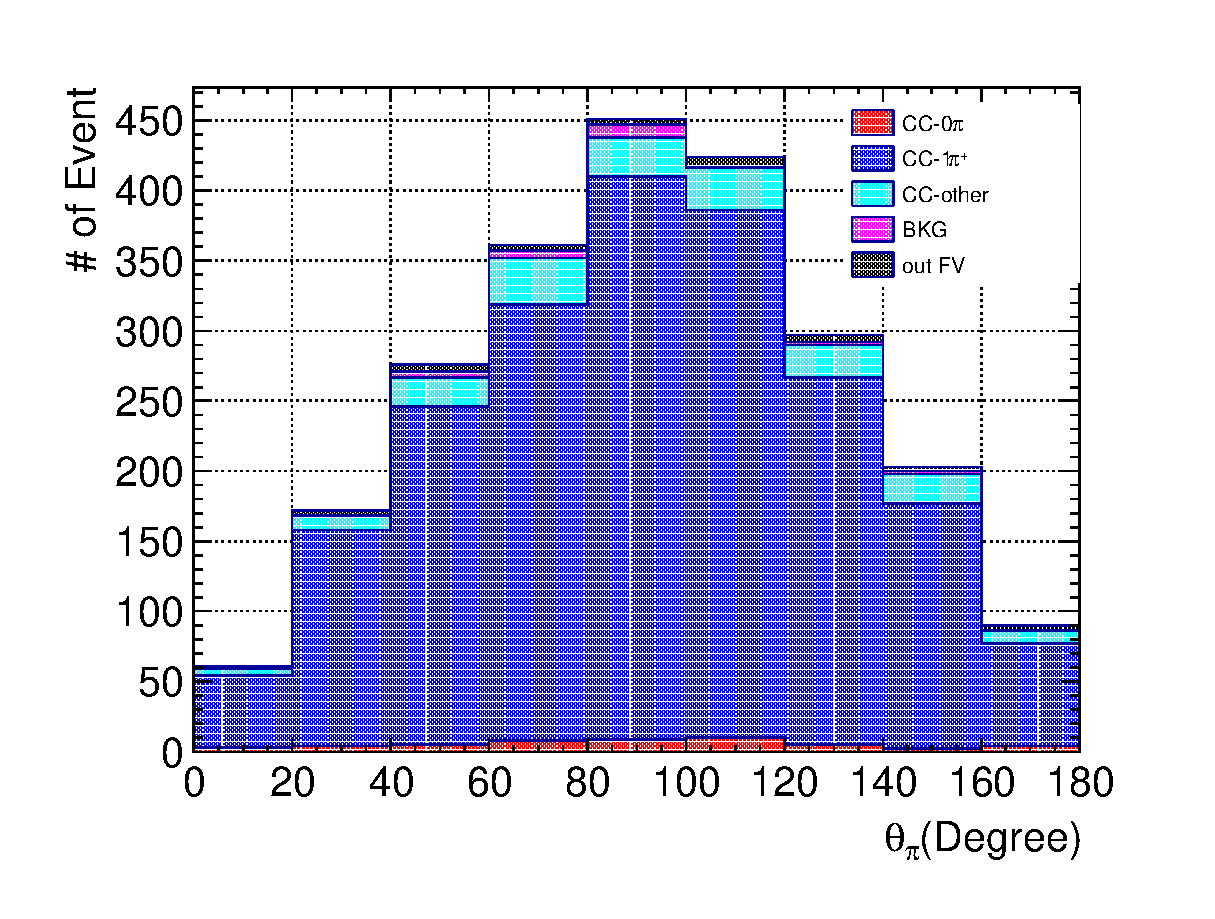
\includegraphics[width=\textwidth]{figures/sel/TPCmu_theta_pi_stack_al9.eps}
                    \caption{TPC-$\mu$: $\tpi$ after track number cut.}
                    \label{subfig:tlpi-tpi-af-trknumcut-tpc}
               \end{subfigure}
               \\
               \begin{subfigure}{\dbfigwid\textwidth}
                    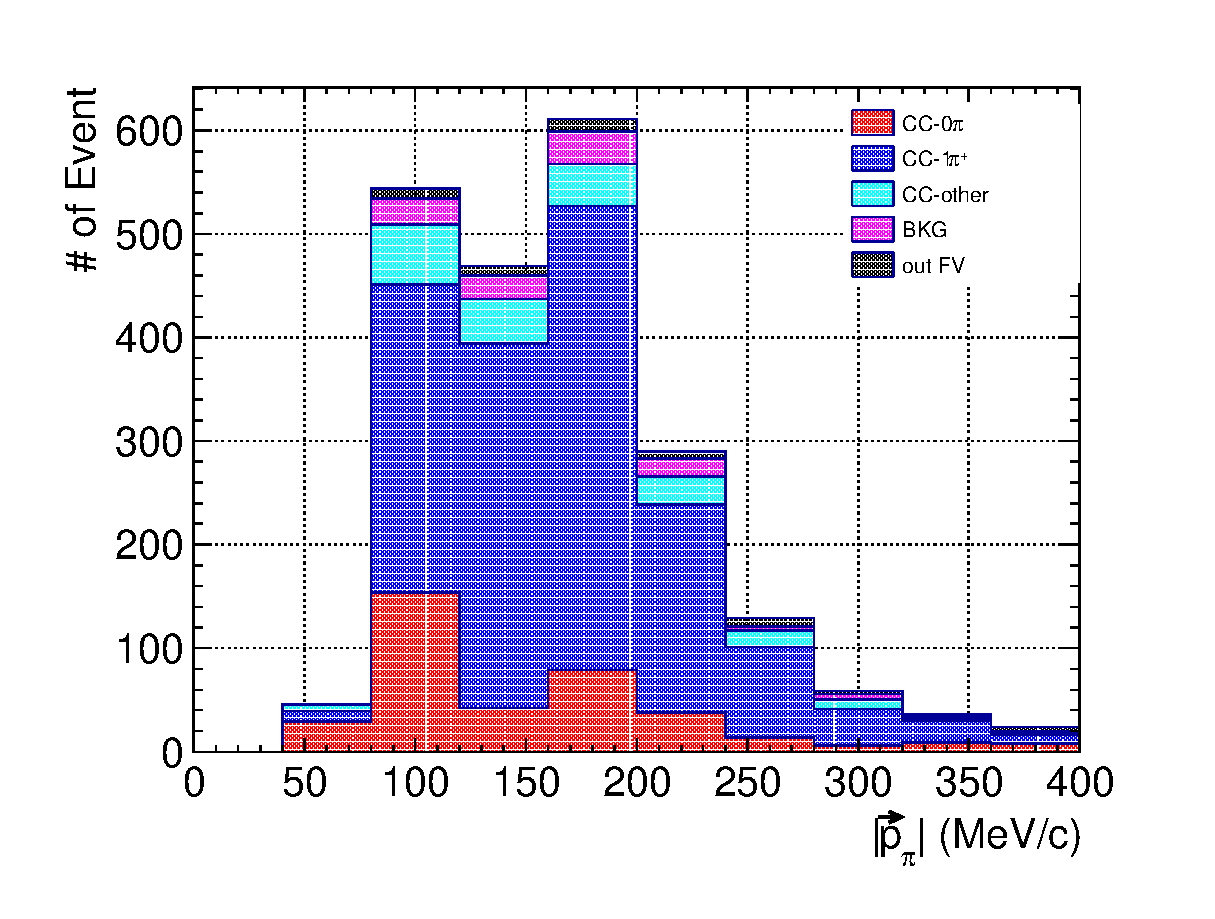
\includegraphics[width=\textwidth]{figures/sel/SFGmu_p_pi_stack_al8.eps}
                    \caption{SFGD-$\mu$: $\ppi$ before track number cut.}
                    \label{subfig:tlpi-ppi-bf-trknumcut-sfg}
               \end{subfigure}
               \begin{subfigure}{\dbfigwid\textwidth}
                    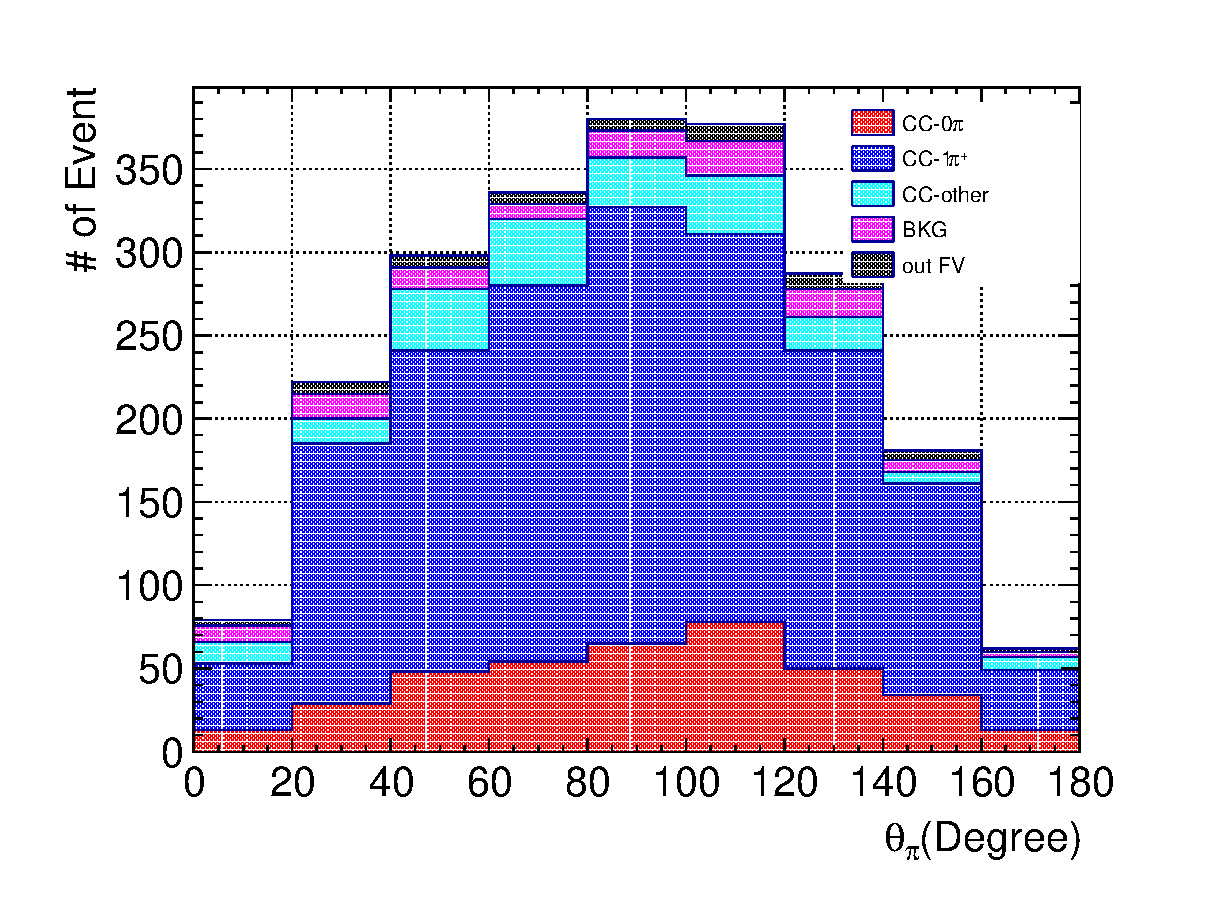
\includegraphics[width=\textwidth]{figures/sel/SFGmu_theta_pi_stack_al8.eps}
                    \caption{SFGD-$\mu$: $\tpi$ before track number cut.}
                    \label{subfig:tlpi-tpi-bf-trknumcut-sfg}
               \end{subfigure}
               \\
               \begin{subfigure}{\dbfigwid\textwidth}
                    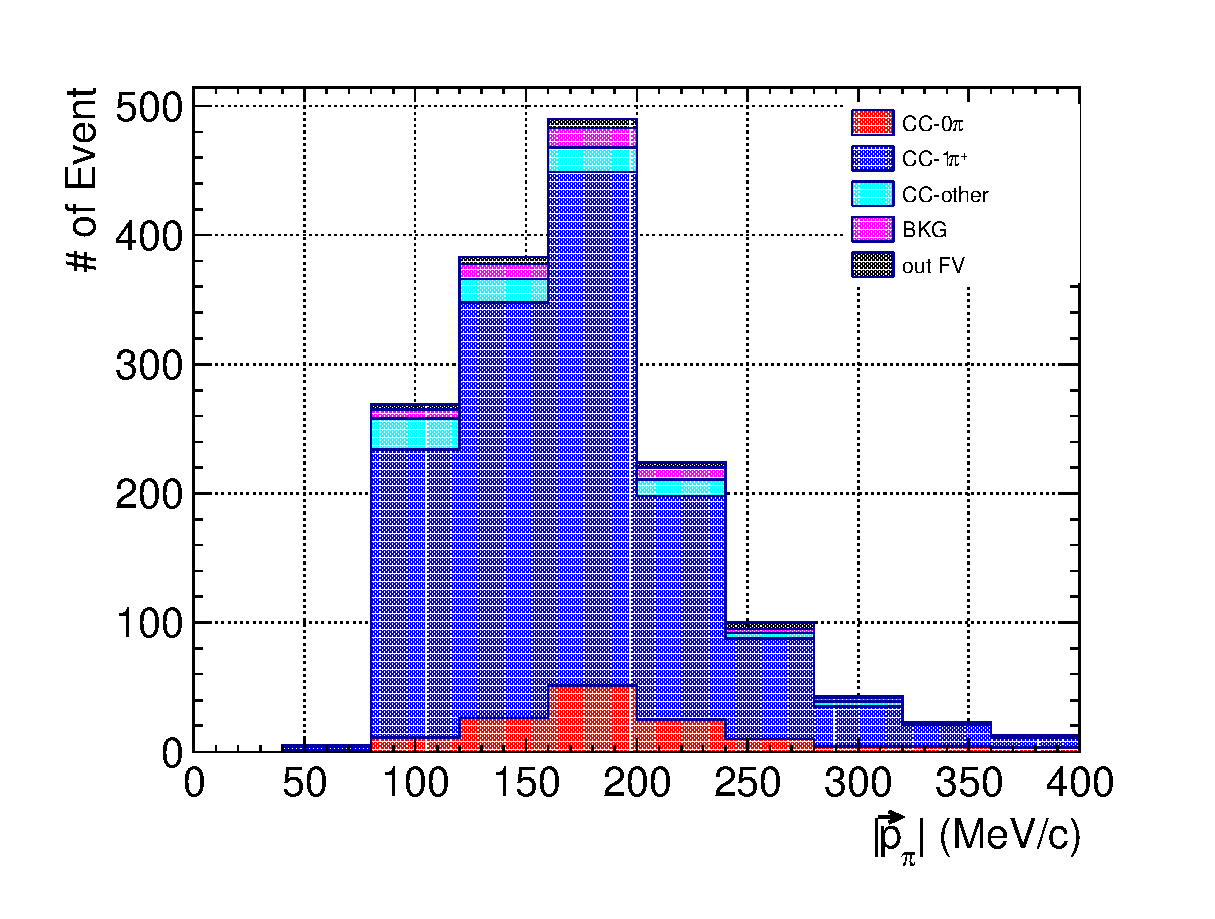
\includegraphics[width=\textwidth]{figures/sel/SFGmu_p_pi_stack_al9.eps}
                    \caption{SFGD-$\mu$: $\ppi$ after track number cut.}
                    \label{subfig:tlpi-ppi-af-trknumcut-sfg}
               \end{subfigure}
               \begin{subfigure}{\dbfigwid\textwidth}
                    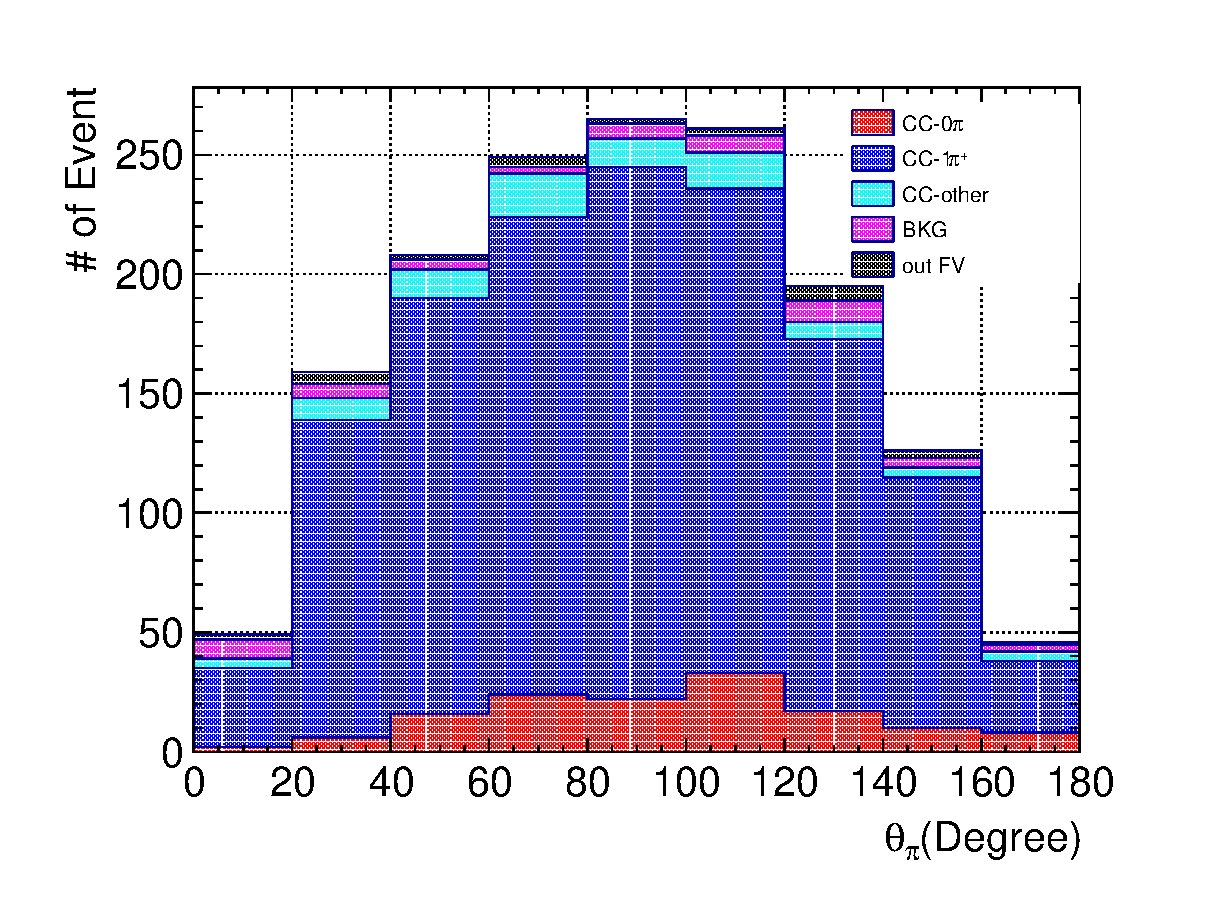
\includegraphics[width=\textwidth]{figures/sel/SFGmu_theta_pi_stack_al9.eps}
                    \caption{SFGD-$\mu$: $\tpi$ after track number cut.}
                    \label{subfig:tlpi-tpi-af-trknumcut-sfg}
               \end{subfigure}
               \caption{Pion kinematics before and after track number cuts.}
               \label{fig:tl-trknum-cut-res}
          \end{figure}

          As shown in Figs.~\ref{subfig:tlpi-ppi-bf-trknumcut-tpc} and \ref{subfig:tlpi-ppi-af-trknumcut-tpc}, the purity of the $\numuccopi$ selection improved from $74.1\%$ to $87.5\%$ after applying the track number cuts for the TPC-$\mu$ sub-sample. 
          Similarly, Figs.~\ref{subfig:tlpi-ppi-bf-trknumcut-sfg} and \ref{subfig:tlpi-ppi-af-trknumcut-sfg} show an improvement in selection purity from $65.9\%$ to $80.7\%$. 
          Although the cuts result in an $18\%$ and $14\%$ decrease in the number of signal events, these results demonstrate that the track number cuts effectively remove backgrounds. 
          Since the HAT-$\mu$ sub-sample still suffers from a global matching problem, its results are not included here.

          For events passing all selection steps, the presence of a primary pion is inferred from the existence of a proper ME candidate, and its momentum is reconstructed by range. 
          A quick consistency check involves plotting the distribution of the time difference between the ME and the primary vertex, which should equal the pion travel time plus the muon decay time. 
          Since the pion travel time is on the order of nanoseconds, the resulting distribution should closely follow the muon exponential decay. 
          The distributions of the ME time delay for the TPC-$\mu$ and SFGD-$\mu$ sub-samples are shown in Fig.~\ref{fig:tlpi-me-td}.
          \begin{figure}
               \centering
               \begin{subfigure}{\dbfigwid\textwidth}
                    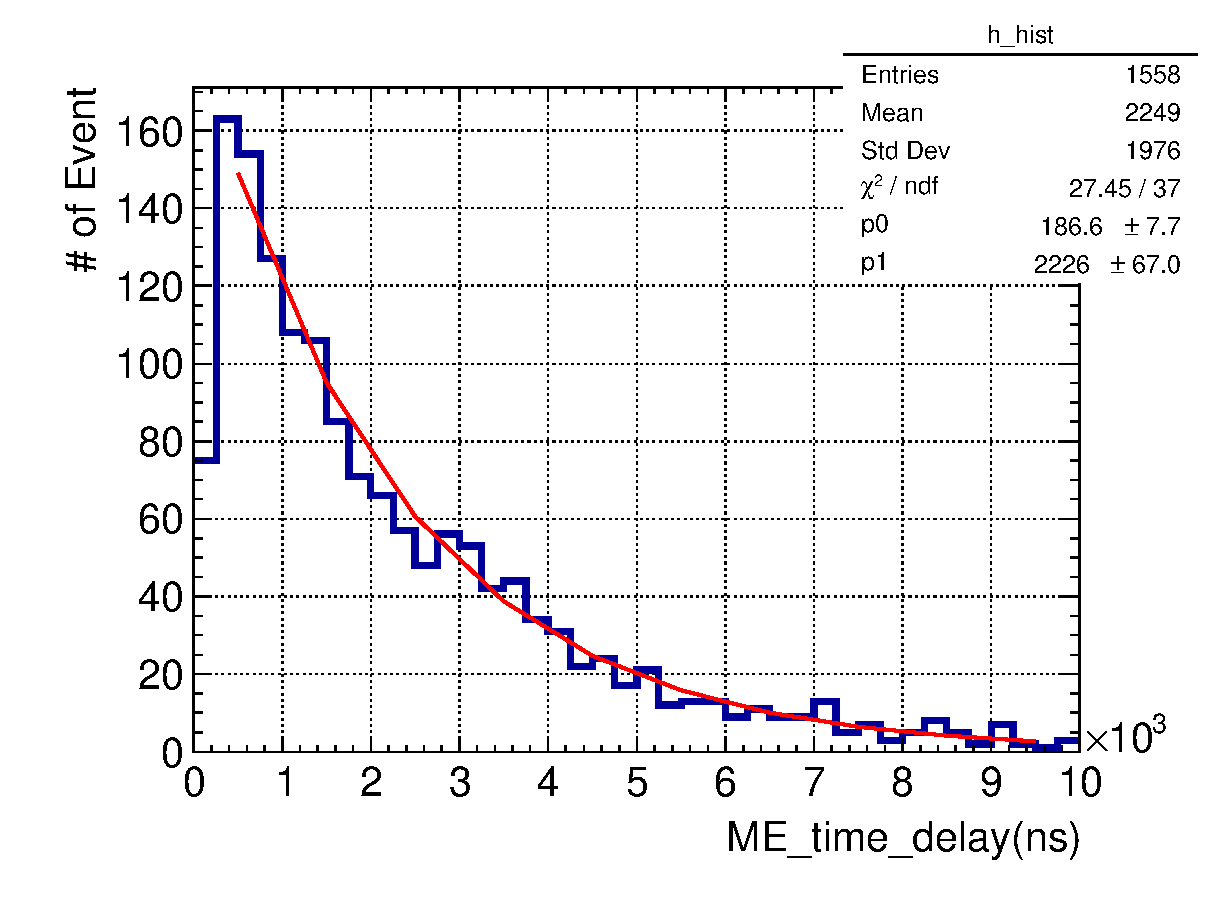
\includegraphics[width=\textwidth]{figures/sel/SFGmu_ME_td_hist_al9_fit.eps}
                    \caption{SFGD-$\mu$. The fitted lifetime is $2226\pm67~\ns$.}
                    \label{subfig:tlpi-me-td-sfgmu}
               \end{subfigure}
               \begin{subfigure}{\dbfigwid\textwidth}
                    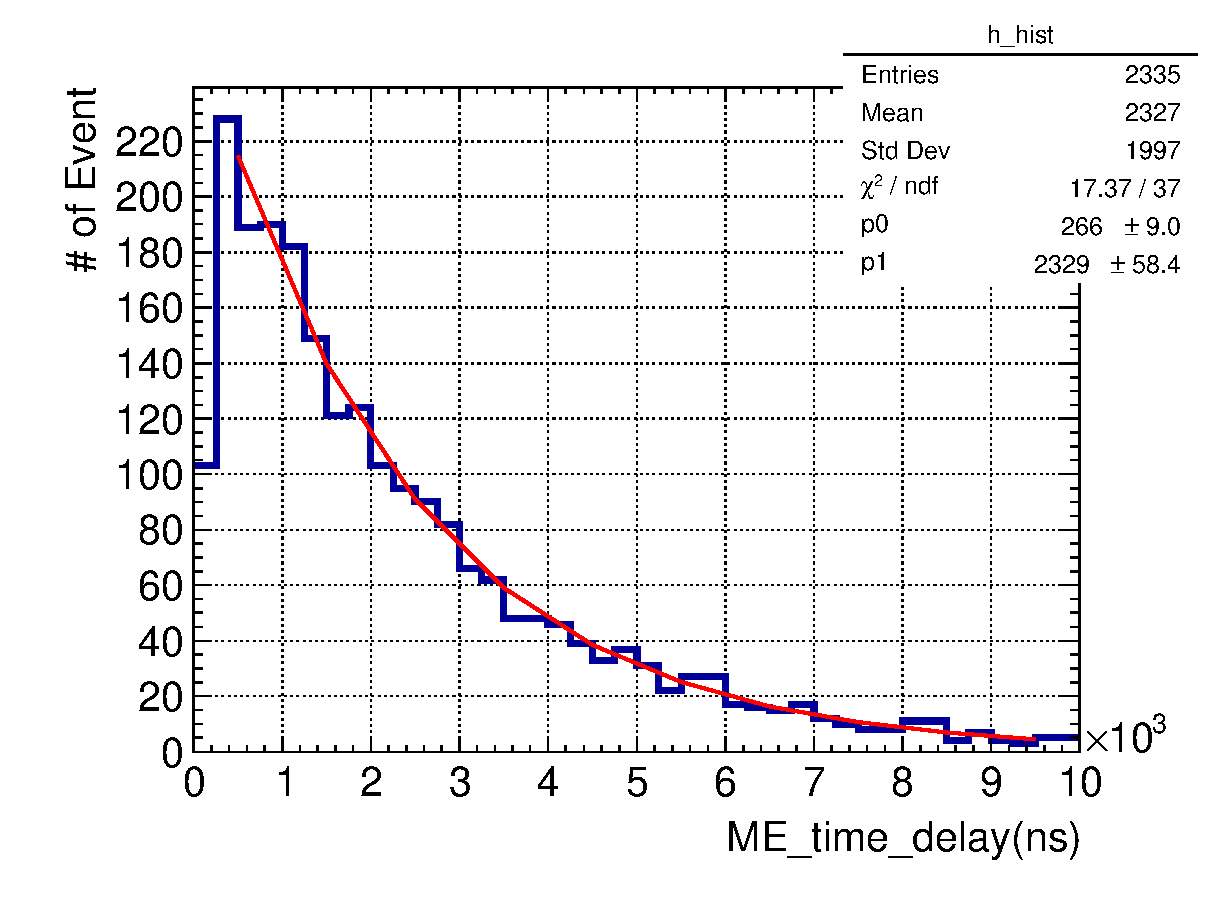
\includegraphics[width=\textwidth]{figures/sel/TPCmu_ME_td_hist_al9_fit.eps}
                    \caption{TPC-$\mu$. The fitted lifetime is $2329\pm58~\ns$.}
                    \label{subfig:tlpi-me-td-tpcmu}
               \end{subfigure}
              \caption{Time difference between ME and the end point of the stopping pion track.}
               \label{fig:tlpi-me-td}
            \end{figure}
          \end{figure}

          Fig.~\ref{fig:cc1pi-tl} displays a candidate $\ccopi$ event passing the $\numuccopi$-TL selection in the upgraded ND280 during the beam run in June 2024. 
          The second-longest track is the ME, whose starting point is very close to that of the primary muon, indicating the extremely short distance traveled by the primary pion. 
          \begin{figure}[!htb] 	
               \centering 		
               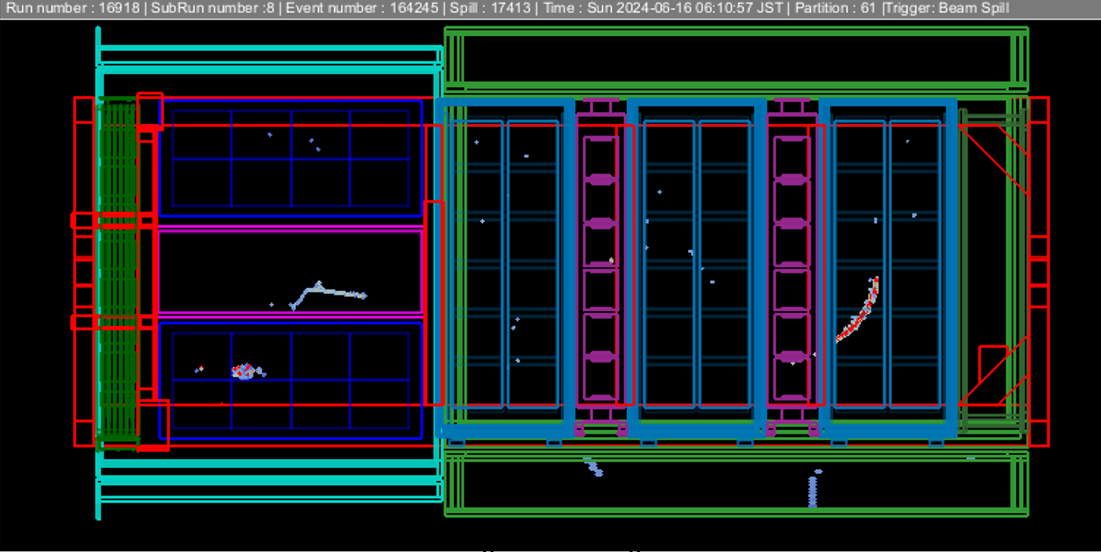
\includegraphics[width=\sgfigwid\textwidth]{figures/shortPion.png}
               \caption{\label{fig:cc1pi-tl} A $\ccopi$-TL candidate event in upgraded ND280, where the long track is the primary muon and the other track is a delayed ME, which implies the exisitence of a very low momentum primary pion.} 
          \end{figure}
          This short distance makes reconstruction using a track-based method impossible.

     \subsection{Comparison with Conventional Method}
     \label{sec:comparison-conventional}

          One key advantage of the trackless technique is its improved reconstruction in the low-momentum phase space. 
          To verify this claim, I compared pion momentum reconstruction using the conventional method, where the pion is identified by a reconstructed track with an attached ME. 
          A preliminary selection based on the conventional method was developed for this comparison. 
          To differentiate between the two pion selections, the trackless technique selection is referred to as $\numuccopi$-TL, while the conventional method selection is referred to as $\numuccopi$-TR.

          The $\numuccopi$-TR selection is based on the $\numucc$-inclusive selection and employs the same background reduction steps as the $\numuccopi$-TL.
          The difference lies in the reconstruction of the primary pion.
          A reconstructed primary track with an attached ME is required.
          No further optimization is performed, ensuring that this selection encompasses the maximally possible phase space.
          The results of the comparison are shown in Fig.~\ref{fig:tltr-comp}\footnote{Note that the result for $\numuccopi$-TL in this figure does not include the implementation of the early energy deposit in choosing the suitable ME candidate, as this comparison was conducted during the early stage of development. 
          Since the main purpose of this comparison is to demonstrate the limitations of the conventional method, the final reconstruction threshold for the $\numuccopi$-TL is presented in Fig.~\ref{fig:piTLres}.}.
          The efficiencies for pions with momentum higher than $100~\mevc$ are similar for both methods.
          Below $100~\mevc$, the improvement brought by the trackless technique is twofold.
          Firstly, the efficiencies below $100~\mevc$ are significantly higher for the trackless technique.
          The efficiency for $\numuccopi$-TR drops drastically below $80~\mevc$.
          Secondly, the momentum threshold in $\numuccopi$-TL extends below $50~\mevc$, which is impossible for the conventional method.
          More encouragingly, this improvement in low momentum efficiency and lower threshold does not compromise selection purity, as shown in Figs.~\ref{subfig:stack-topo-tl} and \ref{subfig:stack-topo-tr}.

          \begin{figure}
               \centering
               \begin{subfigure}{\dbfigwid\textwidth}
                    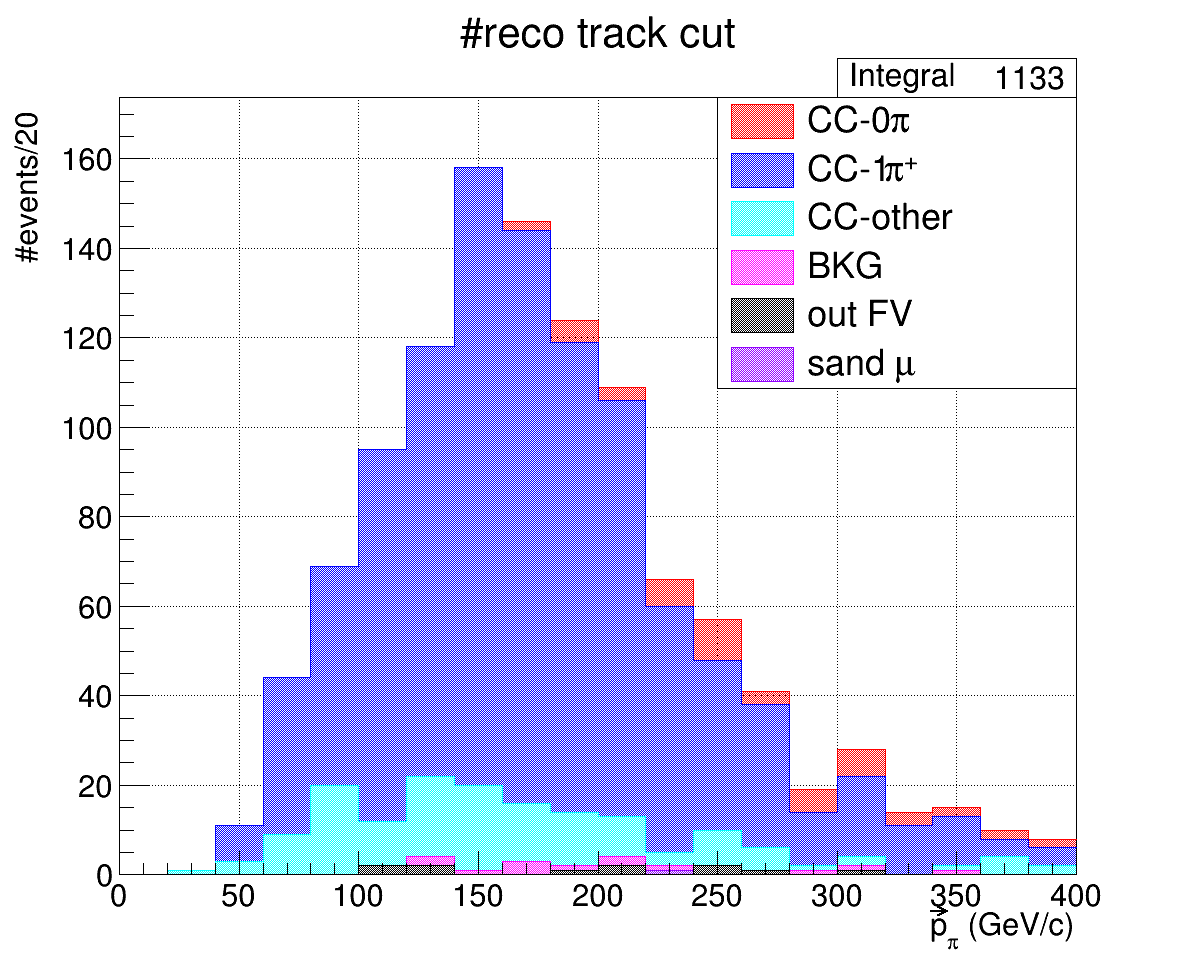
\includegraphics[width=\textwidth]{figures/sel/finhist_pi_mom_topology_TL.png}
                    \caption{$\numuccopi$-TL: Topology decomposition.}
                    \label{subfig:stack-topo-tl}
               \end{subfigure}
               \begin{subfigure}{\dbfigwid\textwidth}
                    \includegraphics[width=\textwidth]{figures/sel/finhist_pi_mom_topology_TR.png}
                    \caption{$\numuccopi$-TL: Topology decomposition.}
                    \label{subfig:stack-topo-tr}
               \end{subfigure}
               \\
               \begin{subfigure}{\dbfigwid\textwidth}
                    \includegraphics[width=\textwidth]{figures/sel/p_pi_eff_al10_TL.png}
                    \caption{$\numuccopi$-TL: Reconstruction efficiency.}
                    \label{subfig:ppi-eff-tl}
               \end{subfigure}
               \begin{subfigure}{\dbfigwid\textwidth}
                    \includegraphics[width=\textwidth]{figures/sel/p_pi_eff_al9_TR.png}
                    \caption{$\numuccopi$-TR: Reconstruction efficiency.}
                    \label{subfig:ppi-eff-tr}
               \end{subfigure}
              \caption{Pion trackless reconstruction results.}
               \label{fig:tltr-comp}
            \end{figure}
          \end{figure}

     \subsection{Impacts on SPK}
          The results of the $\numuccopi$ selection using the trackless pion technique are summarized in Fig.~\ref{fig:piTLres}.
          As shown in Fig.~\ref{fig:ppi-stack}, the trackless selection has achieved its goal of reconstructing low-momentum pions.
          A considerable number of events contain pions with momentum below $100~\mevc$, corresponding to a track length of approximately $50~\textrm{mm}$.
          Moreover, pions with momentum below $80~\mevc$ have also been reconstructed; these pions travel about $30~\textrm{mm}$ and cannot be reconstructed as tracks.
          Furthermore, the momentum-by-range calculation has achieved an excellent resolution of approximately $2\%$, as shown in Fig.~\ref{fig:ppi-res}.
          More encouragingly, the overall efficiencies remain relatively high.
          The step-by-step efficiencies for each selection step are shown in Fig.~\ref{fig:tl-accum-eff}.
          The signal definition used in the calculation requires one true muon that has traveled to the vertical TPC and one true pion that is contained in SFGD.
          Steps 1 to 7 correspond to the $\numucc$-inclusive selection.
          The large drop in efficiency at Step 8 is expected, as it requires exactly one pion to be reconstructed tracklessly.
          All pions undergoing secondary interactions, except for deflection, cannot be reconstructed via this method.
          Hence, the relative efficiency of $0.37/0.66\approx56\%$ is considerably high.
          A further significant drop in efficiency occurs in the next step, the kink cut, which is reasonable as a considerable portion of pions undergo deflection.
          Subsequent drops are graduate cuts to remove backgrounds, resulting in a high purity of $\numuccopi$, as shown in Fig.~\ref{fig:ppi-stack}.

          \begin{figure}[t]
              \centering
              \begin{subfigure}{\trfigwid\textwidth}
                   \includegraphics[width=\textwidth]{figures/sel/ppi_stack.png}
                   \caption{Momentum distribution.}
                   \label{fig:ppi-stack}
              \end{subfigure}
              \begin{subfigure}{\trfigwid\textwidth}
                   \includegraphics[width=\textwidth]{figures/sel/ppi_res.png}
                   \caption{Momentum resolution.}
                   \label{fig:ppi-res}
              \end{subfigure}
              \begin{subfigure}{\trfigwid\textwidth}
                   \includegraphics[width=\textwidth]{figures/sel/INCL_p_pi_accum_eff_al11.png}
                   \caption{Accumulative efficiency.}
                   \label{fig:tl-accum-eff}
              \end{subfigure}
              \caption{Pion trackless reconstruction results.}
              \label{fig:piTLres}
           \end{figure}


    \section{Development of stopping pion control sample}

          \subsection{Implementation}
          \label{sec:sppi-imp}
          Conventionally, selections are used for cross-section analysis, which requires a sufficient portion of all detector systematics to be correctly evaluated.
          However, due to time constraints, this is unlikely to happen within the timeframe of my doctoral study.
          Therefore, only preliminary data–MC comparisons are feasible.
          Nonetheless, because systematic evaluation is an important aspect of cross-section analysis—crucial for improving our understanding of neutrino–nucleus interactions—I implemented the propagation of the momentum-by-range reconstruction systematics for pions tagged by ME.
          To evaluate this systematic, I developed the stopping-pion control sample with the following steps:
          \begin{enumerate}
          \item Find all tracks that contain an SFGD segment and segments in the other sub-detectors.
          \item Check that one end of this track is stopped in SFGD.
          \item Check the PID of this track provided by the other sub-detectors, i.e., HAT or TPC.
          \item Check that there are no other (except ME) near the track end in SFGD.
          \item A final cut requiring the presence of an ME near the track end in SFGD.
          \item Keep only the event with a single stopping-pion candidate.
          \end{enumerate}
          The preliminary result suggests that the control sample consists predominantly of tracks passing HAT and stopping in SFGD.
          Because the current PID in HAT is not fully developed, I investigated further the impact of the log likelihood on pion PID.
          The logarithms of the first and the fourth elements of the pull vector are most relevant.
          For conciseness, these logarithms are simply referred to as the first pull and the fourth pull, respectively.
          For the existing TPC PID, the fourth pull was set to be larger than $0.3$ and the sum of the first and the fourth pull was set to be larger than $0.8$ for pion PID.
          Although HAT is also a TPC, there are design differences, so the PID requirement may differ.
          The distributions of the pulls at HAT for positively charged tracks before any cuts are shown in Fig.~\ref{fig:pulls}, which indicates that a significant fraction of muons will remain after the TPC pull cuts.

          \begin{figure}
               \centering
               \begin{subfigure}{\dbfigwid\textwidth}
                    \includegraphics[width=\textwidth]{figures/sel/sspi_TOP_hat_pid0_stack_al5.eps}
                    \caption{The first pull.}
                    \label{subfig:sppi-pulls-1}
               \end{subfigure}
               \begin{subfigure}{\dbfigwid\textwidth}
                    \includegraphics[width=\textwidth]{figures/sel/sspi_TOP_hat_pid1_stack_al5.eps}
                    \caption{The second pull.}
                    \label{subfig:sppi-pulls-2}
               \end{subfigure}
               \\
               \begin{subfigure}{\dbfigwid\textwidth}
                    \includegraphics[width=\textwidth]{figures/sel/sspi_TOP_hat_pid2_stack_al5.eps}
                    \caption{The third pull.}
                    \label{subfig:sppi-pulls-3}
               \end{subfigure}
               \begin{subfigure}{\dbfigwid\textwidth}
                    \includegraphics[width=\textwidth]{figures/sel/sspi_TOP_hat_pid3_stack_al5.eps}
                    \caption{The fourth pull.}
                    \label{subfig:sppi-pulls-4}
               \end{subfigure}
               \caption{Pull distributions at HAT before any PID cuts for positive reconstructed tracks.}
               \label{fig:pulls}
          \end{figure}

          Hence, stricter cuts are required to obtain a pion sample with higher purity.
          Based on Fig.~\ref{fig:pulls}, a cut on the first, second, and the fourth pull can potentially improve the pion purity.
          A further zoom of the first pull is shown in Fig.~\ref{fig:pull0-zoom}, suggesting a cut to exclude events with the first pull larger than $0.04$.
          \begin{figure}
               \centering
               \includegraphics[width=\textwidth]{figures/sel/sspi_TOP_hat_pid0_stack_al5_zoom.eps}
               \caption{Zoom on the first pull distribution at HAT.}
               \label{fig:pull0-zoom}
          \end{figure}

          However, after the cut on the first pull, the other pull distributions do not show a clear separation between the muon background and the pion signal, as illustrated in Fig.~\ref{fig:pulls-pid0}.
          \begin{figure}
               \centering
               \begin{subfigure}{\dbfigwid\textwidth}
                    \includegraphics[width=\textwidth]{figures/sel/sspi_TOP_hat_pid0_stack_al5_pid0.eps}
                    \caption{The first pull.}
                    \label{subfig:sppi-pulls-1-pid0}
               \end{subfigure}
               \begin{subfigure}{\dbfigwid\textwidth}
                    \includegraphics[width=\textwidth]{figures/sel/sspi_TOP_hat_pid1_stack_al5_pid0.eps}
                    \caption{The second pull.}
                    \label{subfig:sppi-pulls-2-pid0}
               \end{subfigure}
               \\
               \begin{subfigure}{\dbfigwid\textwidth}
                    \includegraphics[width=\textwidth]{figures/sel/sspi_TOP_hat_pid3_stack_al5_pid0.eps}
                    \caption{The fourth pull.}
                    \label{subfig:sppi-pulls-4-pid0}
               \end{subfigure}
               \begin{subfigure}{\dbfigwid\textwidth}
                    \includegraphics[width=\textwidth]{figures/sel/sspi_TOP_trk_heavylen_stack_al5_pid0.eps}
                    \caption{Heavy length.}
                    \label{subfig:sppi-heavylen-pid0}
               \end{subfigure}
               \caption{Pull distributions and a distribution of heavy length at HAT with a cut on the first pull.}
               \label{fig:pulls-pid0}
          \end{figure}

          Instead, I used a concept suggested by my colleague, Xingyu Zhao, from his FGD analysis, where he defined a variable called the heavy length—the portion of the particle inside a dense detector (e.g., SFGD).
          This length can distinguish between leptons and hadrons because hadrons are much more likely to interact with dense material, thereby having shorter lengths within such detectors.
          For the stopping-pion sample, the heavy length is dominated by the portion in the SFGD, as the ECAL and TOF contribute only marginally.
          As shown in Fig.~\ref{subfig:sppi-heavylen-pid0}, a cut on the heavy length to keep events below $150~\mm$ can remove a considerable portion of the muon background remaining after the first-pull cut.

          The pull distributions shown are based on the sub-sample where the pion passes through the Top HAT.
          The Bottom HAT has similar performance, and the same cuts are applied.
          For brevity, the pull distributions for the Bottom HAT are collected in Sec.~\ref{sec:app-bot-pulls} in the Appendix.
          The final selection results for the two subsamples are shown in Fig.~\ref{fig:sppi-kin}.
          The Top HAT subsample has achieved a purity of $96\%$ as shown in Fig.~\ref{subfig:sppi-top-ppi} and Fig.~\ref{subfig:sppi-top-tpi}, which has $91$ $\pip$ signal events, $3$ $\mu^-$, and $2$ $\mu^+$ background events.
          Similarly, the Bottom HAT subsample has achieved a purity of $87\%$ as shown in Fig.~\ref{subfig:sppi-bot-ppi} and Fig.~\ref{subfig:sppi-bot-tpi}, which has $293$ $\pip$ signal events, $15$ $\mu^-$, $26$ $\mu^+$, and $1$ $\pim$ background event.

          \begin{figure}
               \centering
               \begin{subfigure}{\dbfigwid\textwidth}
                    \includegraphics[width=\textwidth]{figures/sel/sspi_TOP_pi_mombr_stack_al6_zoom.eps}
                    \caption{Top HAT $\ppi$.}
                    \label{subfig:sppi-top-ppi}
               \end{subfigure}
               \begin{subfigure}{\dbfigwid\textwidth}
                    \includegraphics[width=\textwidth]{figures/sel/sspi_TOP_theta_trk_stack_al6_zoom.eps}
                    \caption{Top HAT $\tpi$.}
                    \label{subfig:sppi-top-tpi}
               \end{subfigure}
               \\
               \begin{subfigure}{\dbfigwid\textwidth}
                    \includegraphics[width=\textwidth]{figures/sel/sspi_BOT_pi_mombr_stack_al6_zoom.eps}
                    \caption{Bottom HAT $\ppi$.}
                    \label{subfig:sppi-bot-ppi}
               \end{subfigure}
               \begin{subfigure}{\dbfigwid\textwidth}
                    \includegraphics[width=\textwidth]{figures/sel/sspi_BOT_theta_trk_stack_al6_zoom.eps}
                    \caption{Bottom HAT $\tpi$.}
                    \label{subfig:sppi-bot-tpi}
               \end{subfigure}
               \caption{Stopping-pion kinematic distributions decomposed according to true particle type.}
               \label{fig:sppi-kin}
          \end{figure}

          Because the HAT reconstruction is still under development, the values implemented here may be subject to further updates.
          A good consistency check of using the ME method to select the stopping pion is to check the time difference between the ME and the end point of the stopping track.
          This distribution should closely follow the muon exponential decay curve.
          The result is shown in Fig.~\ref{fig:sppi-me-td}.

          \begin{figure}
               \centering
               \begin{subfigure}{\dbfigwid\textwidth}
                    \includegraphics[width=\textwidth]{figures/sel/sspi_TOP_ME_td_hist_al6_sfgfinposfit_comb.eps}
                    \caption{MC. The fitted lifetime is $2335\pm132~\ns$.}
                    \label{subfig:sppi-me-td-mc}
               \end{subfigure}
               \begin{subfigure}{\dbfigwid\textwidth}
                    \includegraphics[width=\textwidth]{figures/sel/sspi_TOP_ME_td_hist_al6_sfgfinpos_fit.eps}
                    \caption{Data. The fitted lifetime is $2234\pm456~\ns$.}
                    \label{subfig:sppi-me-data}
               \end{subfigure}
               \caption{Time difference between ME and the end point of the stopping-pion track.}
               \label{fig:sppi-me-td}
          \end{figure}

          \subsection{Systematics evaluation}
          \label{sec:sppi-syst}
          The control sample is developed with evaluation of the pion momentum by range reconstruction in mind.
          Although the selection is not finalized as the HAT reconstruction and global track matching are still subjected to changes, it is still valuable to develop the systematics evaluation framework.
          One is the to learn the method of performing systematics evaluation, the other is to get a first glimpse of the performance of the pion momentum reconstruction in SFGD.

          The systematics evaluation follows that in the FGD analysis as outlined in Ref.~\cite{Jenkins:2022ljx}.
          While it is straightforward to examine the reconstruction resolution with MC studies, there is no truth information when analysing data.
          As the momentum reconstruction in TPCs has good resolution and is well validated, i.e. there is good agreement between MC and data, instead of comparing the reconstructed momentum to the true momentum, it can be used as a good estimation of the true momentum.
          Moreover, as the control sample selects pion tracks that travel from HAT into SFGD and the pion loses an inifinitesimal amount of energy in the HAT, the momentum obtained from the HAT reconstruction is a good approximation of the true enter momentum in SFGD.
          The devaitions of the SFGD reconstructed moentum from the HAT reconstructed momentum can be computed for both MC and data.
          On one hand, this deviation can be regarded as an approximation of the SFGD momentum resolution.
          On the other hand, the difference between the deviations of MC and data can assess the difference in the reconstruction performance between MC and data in SFGD, i.e. the systematics related to the SFGD momentum by range reconstruction.

          The distributions of the deviations for MC and data are shown in Fig.~\ref{fig:sppi-res} and the fitting parameters, the mean ($x_0$) and the half width half maximum ($\gamma$), are summarised in Table.~\ref{tab:sppi-res}.

          \begin{table}[htbp]
          \centering
          \begin{tabular}{c|cccc}
                       & MC-$x_0~(\mevc)$ & MC-$\gamma$~($\mevc$) & Data-$x_0~(\mevc)$ & Data-$\gamma$~($\mevc$)\\
          \hline
          FGD & $-25.03 \pm 0.52$ & $85.38 \pm 1.20$ & $-19.43 \pm 1.41$ & $93.57 \pm 4.15$ \\
          SFGD & $-5.29 \pm 0.73$  & $7.49 \pm 0.65$  & $-10.14 \pm 4.55$  & $16.34 \pm 5.21$ \\
          \end{tabular}
          \caption{Fit parameters for the momentum deviation distributions.}
          \label{tab:sppi-res}
          \end{table}

          Both widths are significantly smaller than those in the FGD analysis presented in Ref.~\cite{Jenkins:2022ljx}, in the FGD study.
          However, due to the limited amount of data, the difference between the two distributions is still relatively large that the magnitude of the average systematic error, about $3\%$ to $5\%$, is slightly larger than that in the FGD analysis, about $2\%$. 
          However, the relative error in the first bin, i.e., for the low-momentum pions ($\ppi<100~\mevc$), about $6\%$ to $9\%$, is considerably smaller than the FGD analysis, about $10\%$ to $14\%$.
          \begin{figure}[h]
          \centering
          \begin{subfigure}[h]{\dbfigwid\textwidth}
          \centering
          \includegraphics[width=\textwidth]{figures/sel/sspi_TOP_pi_mombr_hatp_difhist_al6_mc.eps}
          \caption{Momentum difference between SFGD and HAT for MC.}
          \label{subfig:sfgp-hatp-dif-mc}
          \end{subfigure}
          \hfill
          \begin{subfigure}[h]{\dbfigwid\textwidth}
          \centering
          \includegraphics[width=\textwidth]{figures/sel/sspi_TOP_pi_mombr_hatp_difhist_al4_CombHAT_data.eps}
          \caption{Momentum difference between SFGD and HAT for data.}
          \label{subfig:sfgp-hatp-dif-data}
          \end{subfigure}
          \caption{Momentum difference for stopping pion control sample.}
          \label{fig:sppi-res}
          \end{figure}

          The systematic error paramters are then passed to the HighLAND framework, the selection development and systematics propagation software used at T2K, to propagate the uncertainty through the $\numuccopi$-TL selection.
          The result is shown in Fig.~\ref{fig:tlpi-relerr}.
          \begin{figure}[h]
          \centering
          \begin{subfigure}[h]{\dbfigwid\textwidth}
          \centering
          \includegraphics[width=\textwidth]{figures/sel/relerr-tpcmu.png}
          \caption{Relative error for the TPC-$\mu$ sub-sample.}
          \label{subfig:relerr-tpcmu}
          \end{subfigure}
          \hfill
          \begin{subfigure}[h]{\dbfigwid\textwidth}
          \centering
          \includegraphics[width=\textwidth]{figures/sel/relerr-sfgmu.png}
          \caption{Relative error for the SFGD-$\mu$ sub-sample.}
          \label{subfig:relerr-sfgmu}
          \end{subfigure}
          \caption{Relative error for the $\numuccopi$-TL selection.}
          \label{fig:tlpi-relerr}  
          \end{figure}
          Due to the incompleteness of global reconstruction and the limited amount of data, this error propagation is performed with only $20$ toys, which can only serve as a proof of the succesful propagation of the systematics.
          Even though no phyics conclusion can be drawn with this limited amount of data, it is promising to observe a considerable decrease in the error for the low momentum pion, comparing to the FGD analysis, showcasing the strength of SFGD and the trackless reconstruction technique.

     \section{Data-MC comparisons}
          Conventionally, kinematic distributions from these selections will be extracted and passed through the unfolding process which maps the reconstructed variables to the truth space. 
          These unfolded distributions can then be used to compare directly with output from MC event generators.
          However, the unfolding process needs to account for all major detector effects, and unfortunately, a full coverage of systematics for the new sub-detectors is not possible within my doctoral study timeline.
          Hence, I have to resort to a reconstruction-level Data-MC comparisons instead.
          Although the comparison result will only be valid for the specific configurations of interaction model used to produce the MC sample, it is the only possible way to utilize the collected data to produce physical results.
     
          With the development of the pion momentum by range reconstruction systematics, it is possible to take a first glimpse of data-MC comparisons for the $\numuccopi$-TL selection. 
          As the global reconstruction is yet to be finalized and only one preliminary systematics is propagated, this data-MC comparison is merely a demonstration of how the data can be used in the future analysis, and no physics conclusion should be drawn.
          The data-MC comparisons are shown in Fig.~\ref{fig:tlpi-datamc}.
          It is reassuring to observe no significant discrepancy between data and MC in the $\numuccopi$-TL selection.
          The data-MC comparison workflow is thus complete.
          Official analysis results can be readily obtained once the various systematics are in place by putting both MC and data through the $\numuccopi$-TL selection.
          \begin{figure}[h]
               \centering
               \begin{subfigure}{\dbfigwid\textwidth}
                    \includegraphics[width=\textwidth]{figures/sel/datamc-comp-ppi-tpcmu.png}
                    \caption{The TPC-$\mu$ sub-sample: $\ppi$.}
                    \label{subfig:datamc-tpcmu}
               \end{subfigure}
               \begin{subfigure}{\dbfigwid\textwidth}
                    \includegraphics[width=\textwidth]{figures/sel/datamc-comp-ppi-sfgmu.png}
                    \caption{The SFGD-$\mu$ sub-sample: $\ppi$.}
                    \label{subfig:datamc-sfgmu}
               \end{subfigure}
               \\
               \begin{subfigure}{\dbfigwid\textwidth}
                    \includegraphics[width=\textwidth]{figures/sel/datamc-comp-tpi-tpcmu.png}
                    \caption{The TPC-$\mu$ sub-sample: $\theta$.}
                    \label{subfig:datamc-theta-tpcmu}
               \end{subfigure}
               \begin{subfigure}{\dbfigwid\textwidth}
                    \includegraphics[width=\textwidth]{figures/sel/datamc-comp-tpi-sfgmu.png}
                    \caption{The SFGD-$\mu$ sub-sample: $\theta$.}
                    \label{subfig:datamc-theta-sfgmu}
               \end{subfigure}
               \caption{Data-MC comparisons for the $\numuccopi$-TL selection.}
               \label{fig:tlpi-datamc}
          \end{figure}

     \section{Discussion}
     \label{sec:technique-disc}
          The two new techniques elaborated in this chapter, the ESC selection and the pion trackless reconstruction, have shown significant improvement in the reconstruction of hadrons in SFGD.
          One leads to a $50\%$ improvement in the momentum resolution of protons, while the other significantly improves the low momentum pion reconstruction efficiency and extends the pion reconstruction threshold to $50~\mevc$, which is impossible for the conventional method.
          Both the $\numuccopi$ and ESC proton selections are finished for primary muons going into the vertical TPC and SFGD. 
          The sub-sample for muons going into HAT is missing as the global reconstruction matching for tracks passing through HAT is still under development.
          However, as the two new techniques in this chapter are developed for hadrons, the performance should not depend on the ending position of the muons.
          Hence, reconstruction improvement showcased in this chapter should be applicable to the muons going into HAT as well.
          With this improvement in the single particle kinematics, it is exciting to see the performance of the reconstruction of the higher level variables, such as the TKI variables, in the next chapter.